\documentclass[oneside]{book}
%\documentclass{book}
%If you're going to print this, perhaps get ride of oneside so that \parts{} will have their own page!
\title{
	\begin{huge}
		\bf{Everything You Need To Know About MAT436}
	\end{huge}
	}
\author{Nathanael Chwojko-Srawley}
%\date{} % If you want to specify a date
\usepackage{inputenc}         % Used to compile any UTF-8 Character (and supports Unicode)
\usepackage{extarrows}         % Used to compile any UTF-8 Character (and supports Unicode)
\usepackage{stackengine}
\usepackage{amsmath, amssymb} % Used to write better mathematical expressions (ex. \mathbb{R})
\usepackage{stackrel}         % for left-right arrows, staking symbol above and bellow
\usepackage{mathrsfs}
\usepackage{euscript}
\usepackage[font=itshape]{quoting}
\usepackage{mathtools}
	\usepackage{enumitem}
\usepackage{amsthm}           % Used to create theorem enviroments.
\usepackage{graphicx}         % Let's you use images in LaTeX; ex the \includegraphics command.
\usepackage{hhline}
%\usepackage{luatexja}
% \usepackage{fontspec}
\usepackage{dsfont}
\usepackage{wasysym}          % emoji's!
\usepackage{float}            % package with ``H'' for figures and tables, ex. Images, tables, etc
%\usepackage{subcaption}      % More options with sub-captions.
\usepackage{setspace}         % More flexibility on spacing in document.
\usepackage{hyperref}         % let's me put hyperlinks
%\usepackage{tikz}             % for commutative diagrams https://tex.stackexchange.com/questions/419221/how-to-do-the-pushout-with-universal-property
\usepackage{tikz-cd}          % for commutative diagrams https://tex.stackexchange.com/questions/419221/how-to-do-the-pushout-with-universal-property
%\usepackage{quiver}           % for better commutative diagrams
\usepackage{bookmark}         % creating heading shortcut bar on the left as in word
\usepackage{longtable}        % create tables that extend past one page
%\usepackage{siunitx}         % required for alignment
%\usepackage{multirow}        % for multiple rows
\usepackage{microtype}        % makes nice text. Fixes some under-/over- filled box problems.
%\usepackage{fancyvrb}        % Let's you write code (different style than listings).
\usepackage{tcolorbox} 	      % Makes nice boxes for thms, cor, prop, or anything else.
%\usepackage{enumitem}        % More flexibility on enumeration (don't know much).
\usepackage{xcolor}           % Colour text.
\usepackage{wrapfig}          % To wrap text around figure
\usepackage{listings}         % Create nice colour code blocks (customized in preamble)
\usepackage{biblatex}
\usepackage{thmtools}         % Customize theorem environment (in preamble).
%\usepackage{marvosym}        % Provide ``basic'' symbols (hazard, religious, smiley face etc.)
\usepackage{array}            % \begin{table}{>{\em}c c} -> 1st column italic (bfseries for bold)
%\usepackage[english]{babel}  % If I want to blindtext in english.
\usepackage{blindtext}
\usepackage[a4paper, total={6in, 8in}]{geometry}
%\usepackage[symbol]{footmisc} % For daggers and asteriks for footnoes. 1: *, 2: dagger, etc.
\usepackage{fancyhdr}
\usepackage{titlesec}
%\usepackage{pst-plot}          %To make nice plots: https://tex.stackexchange.com/questions/47594/how-can-i-make-a-graph-of-a-function#47596
\usepackage[answerdelayed]{exercise}
\usepackage{cleveref}           %This package must be loaded after any other package that touches refereneces, so it
									%should bassically be the last one to load
\usepackage{etoolbox}          % for Dynkin diagrams
\usepackage{dynkin-diagrams}   % for Dynkin diagrams

\usepackage{markdown}

%header information
\pagestyle{fancy}
\setlength\headheight{20pt}
\renewcommand{\sectionmark}[1]{\markright{\thesection.\ #1}}
\renewcommand{\chaptermark}[1]{\markboth{#1}{}}
\fancyfoot[C,CO]{\textcolor{gray}{Nathanael Chwojko-Srawley}}
\fancyfoot[R,RO]{\thepage}{}

\titleformat
{\chapter} % command
[display] % shape
{\bfseries\Huge\itshape} % format
{\thechapter} % label
{0.5ex} % sep
{
    \rule{\textwidth}{1pt}
    \vspace{1ex}
    \centering
} % before-code
[
\vspace{-0.5ex}%
\rule{\textwidth}{0.3pt}
] % after-code
%https://tex.stackexchange.com/questions/826/symbols-instead-of-numbers-as-footnote-markers#830
%\bibliography{mybasictex}
%\bibliographystyle{ieeetr}   %ieeetr, apalike, mlalike.
%Note that if you want to enumerate with custom or no labels, do
%\begin{enumerate}[label={HERE}]

%example of tick-cd package:
%\begin{tikzcd}
%A \arrow[d,"f"'] \arrow[r,"g"] &
%C \arrow[d,"\beta"'] \arrow[ddr,bend left,"\beta'"] \\
%B \arrow[r,"\alpha"] \arrow[drr,bend right,"\alpha'"'] &
%D \arrow[dr,dashed,"\theta"] \\
%&& Y
%\end{tikzcd}

%Exercices Code: see https://tex.stackexchange.com/questions/369265/math-book-how-to-write-exercise-and-answers

\stackMath %to be able to stack text in math mode
% For devnagari font for that one example
% \newcommand\dn{\catcode`\~=12
%            \fontspec[Script=Devanagari,Mapping=velthuis-sanskrit]{Nakula}}


%\ExerciseLevelInToc
\counterwithin{Exercise}{section}
\counterwithin{Answer}{section}
%\renewcommand{\ExerciseHeader}{\noindent\def\stackalignment{c}% code from https://tex.stackexchange.com/a/195118/101651
    %\stackunder{{\textbf{\large\ExerciseName}}}{\textcolor{black}{\rule{40pt}{4pt}}}\medskip}



%theorem code
\definecolor{dkgreen}{rgb}{0,0.6,0}
\definecolor{gray}{rgb}{0.5,0.5,0.5}
\definecolor{mauve}{rgb}{0.58,0,0.82}
\definecolor{lightyellow}{rgb}{1,1,0.6}
\definecolor{reddish}{HTML}{A01A3A}
%Theorems, propositions, Corollaries, Definitions
\tcbuselibrary{theorems}
\newtcbtheorem[number within=section]{thm}{Theorem}%
{colback=green!5,colframe=green!35!black,fonttitle=\bfseries}{th}
\newtcbtheorem[number within=section]{lem}{Lemma}%
{colback=blue!5,colframe=black!35!black,fonttitle=\bfseries}{lm}
\newtcbtheorem[number within=section]{defn}{Definition}%
{colback=red!5,colframe=red!35!black,fonttitle=\bfseries}{df}
\newtcbtheorem[number within=section]{axiom}{Axiom}%
{colback=black!5,colframe=yellow!35!black,fonttitle=\bfseries}{ax}
\newtcbtheorem[number within=section]{prop}{Proposition}%
{colback=white!5,colframe=white!35!black,fonttitle=\bfseries}{pr}
\newtcbtheorem[number within=section]{cor}{Corollary}%
{colback=blue!5,colframe=blue!35!black,fonttitle=\bfseries}{co}



%\newtcbtheorem[number within=section]{thm}{Theorem}%
%{colback=green!5,colframe=green!35!black,fonttitle=\bfseries}{th}
%\newtcbtheorem[number within=section]{lem}{Lemma}%
%{colback=black!5,colframe=black!35!black,fonttitle=\bfseries}{lm}
%\newtcbtheorem[number within=section]{defn}{Definition}%
%{colback=red!5,colframe=red!35!black,fonttitle=\bfseries}{df}
%\newtcbtheorem[number within=section]{prop}{Proposition}%
%{colback=white!5,colframe=white!35!black,fonttitle=\bfseries}{pr}
%\newtcbtheorem[number within=section]{cor}{Corollary}%
%{colback=blue!5,colframe=blue!35!black,fonttitle=\bfseries}{co}

\declaretheoremstyle[
spaceabove=6pt, spacebelow=6pt,
headfont=\normalfont\bfseries,
notefont=\mdseries, notebraces={(}{)},
bodyfont=\normalfont,
postheadspace=1em,
numberwithin=section
]{exstyle}

\declaretheoremstyle[
spaceabove=6pt, spacebelow=6pt,
headfont=\normalfont\bfseries,
notefont=\mdseries, notebraces={(}{)},
bodyfont=\normalfont,
postheadspace=1em,
headpunct={},
qed=$\blacktriangledown$,
numbered=no
]{solstyle}

\declaretheoremstyle[
spaceabove=6pt, spacebelow=6pt,
headfont=\normalfont\bfseries,
notefont=\mdseries, notebraces={(}{)},
bodyfont=\normalfont,
postheadspace=1em,
headpunct={},
numbered=no
]{questyle}

\declaretheorem[style=solstyle]{solution}
\declaretheorem[style=questyle]{question}
%\declaretheorem[style=solstyle]{remark} (got a ``Note'' enviroment at the bottom``)
%\declaretheorem[style=solstyle]{intuition}


%shortcuts for this file (newcommand and renewcommand)


% Custom Commands
\newcommand{\A}{\mathbb{A}}
\newcommand{\F}{\mathbb{F}}
\newcommand{\N}{\mathbb{N}}
\newcommand{\Q}{\mathbb{Q}}
\newcommand{\R}{\mathbb{R}}
\newcommand{\V}{\mathbb{V}}
\newcommand{\Z}{\mathbb{Z}}
\newcommand{\C}{\mathbb{C}}
\renewcommand{\H}{\mathbb{H}}

\newcommand{\CA}{\mathcal{A}}
\newcommand{\CB}{\mathcal{B}}
\newcommand{\CC}{\mathcal{C}}
\newcommand{\CD}{\mathcal{D}}
\newcommand{\CF}{\mathcal{F}}
\newcommand{\CG}{\mathcal{G}}
\newcommand{\CH}{\mathcal{H}}
\newcommand{\CI}{\mathcal{I}}
\newcommand{\CL}{\mathcal{L}}
\newcommand{\CN}{\mathcal{N}}
\newcommand{\CO}{\mathcal{O}}
\newcommand{\CP}{\mathbb{C}\mathrm{P}}
\newcommand{\CQ}{\mathcal{Q}}
\newcommand{\CR}{\mathcal{R}}
\newcommand{\CK}{\mathcal{K}}
\newcommand{\CS}{\mathcal{S}}
\newcommand{\CT}{\mathcal{T}}
\newcommand{\CV}{\mathcal{V}}
\newcommand{\CZ}{\mathcal{Z}}
\newcommand{\ff}{\mathscr{F}}
\newcommand{\EF}{\EuScript{F}}
\newcommand{\EO}{\EuScript{O}}
\newcommand{\EC}{\EuScript{C}}
\newcommand{\EH}{\EuScript{H}}
\newcommand{\EL}{\EuScript{L}}
\newcommand{\EM}{\EuScript{M}}
\newcommand{\ET}{\EuScript{T}}

\newcommand{\sse}{\subseteq}
\newcommand{\nsse}{\not\subseteq}
\newcommand{\ssne}{\subsetneq}
\newcommand{\qn}{\quad\newline}
\newcommand{\placeholder}{\_\_\_\_\_}
\newcommand{\subg}{\leqslant}
%\newcommand{\subgne}{\lneqslant}
\newcommand{\supg}{\geqslant}
\newcommand{\nsubg}{\trianglelefteq}
\newcommand{\csubg}{\blacktriangleleft}
\newcommand{\nsupg}{\trianglerighteq}
\newcommand{\isosubg}{\lesssim}
\renewcommand{\mid}{\big|}
\renewcommand{\phi}{\varphi}

\newcommand{\oln}{\overline}
\renewcommand{\bf}[1]{\textbf{#1}}

\newcommand{\ev}{\operatorname{ev}}
\renewcommand{\sp}{\operatorname{sp}}
\newcommand{\tr}{\operatorname{tr}}
\newcommand{\op}{\operatorname{op}}
\newcommand{\ad}{\operatorname{ad}}
\newcommand{\im}{\operatorname{im}}
\newcommand{\id}{\operatorname{id}}
\newcommand{\ch}{\operatorname{ch}}
\newcommand{\GL}{\operatorname{GL}}
\newcommand{\rad}{\operatorname{rad}}
\newcommand{\Gal}{\operatorname{Gal}}
\newcommand{\Rep}{\operatorname{Rep}}
\newcommand{\Aut}{\operatorname{Aut}}
\newcommand{\Sym}{\operatorname{Sym}}
\newcommand{\Mod}{\operatorname{Mod}}
\newcommand{\Grp}{\operatorname{Grp}}
\newcommand{\Hom}{\operatorname{Hom}}
\newcommand{\Emb}{\operatorname{Emb}}
\newcommand{\Ext}{\operatorname{Ext}}
\newcommand{\End}{\operatorname{End}}
\newcommand{\Inn}{\operatorname{Inn}}
\newcommand{\Ind}{\operatorname{Ind}}
\newcommand{\Out}{\operatorname{Out}}
\newcommand{\Jac}{\operatorname{Jac}}
\newcommand{\Nil}{\operatorname{Nil}}
\newcommand{\Tor}{\operatorname{Tor}}
\newcommand{\Ann}{\operatorname{Ann}}
\newcommand{\Syl}{\operatorname{Syl}}
\newcommand{\conj}{\operatorname{conj}}
\newcommand{\kdim}{\operatorname{kdim}}
\newcommand{\coker}{\operatorname{coker}}
\newcommand{\Obj}[1]{\operatorname{Obj}(\textbf{#1})}
\newcommand{\Mor}[1]{\operatorname{Mor}(\textbf{#1})}
\newcommand{\Frac}{\operatorname{Frac}}
\newcommand{\Spec}{\operatorname{Spec}}
\newcommand{\rank}{\operatorname{rank}}
\renewcommand{\index}{\operatorname{index}}
\newcommand{\mSpec}{\operatorname{mSpec}}
\newcommand{\Tens}[1]{#1\otimes \_\_}
\newcommand{\Char}{\operatorname{char}}
\newcommand{\Span}{\operatorname{span}}
\newcommand{\Dlim}{\lim\limits_{\longrightarrow}}
\newcommand{\coDlim}{\lim\limits_{\longleftarrow}}
\newcommand{\fHom}[1]{\operatorname{Hom}(#1, \_\_)}
\newcommand{\cofHom}[1]{\operatorname{Hom}(\_\_, #1)}
\newcommand{\trdeg}{\operatorname{trdeg}}
\newcommand{\acton}{\curvearrowright}
\newcommand{\actson}{\curvearrowright}

\renewcommand{\Re}{\operatorname{Re}}
\renewcommand{\Im}{\operatorname{Im}}

%for saturated ideals in the localization section
\newcommand{\LIm}{{}^{\iota} }
\newcommand{\LPre}{{}^{\pi} }

% Arrows
\newcommand{\rw}{\rightarrow}
\newcommand{\wto}{\rightharpoonup}
\newcommand{\rrw}{\rightrightarrows}
\newcommand{\Rw}{\Rightarrow}
\newcommand{\lw}{\leftarrow}
\newcommand{\Lw}{\Leftarrow}
\newcommand{\lrw}{\leftrightarrow}
\newcommand{\LRw}{\Leftrightarrow}

\newcommand{\dcup}{\sqcup}
\newcommand{\Dcup}{\bigsqcup}
\newcommand{\set}[2]{\left\{#1 \ \middle|\ #2\right\}}

\newcommand\mapsfrom{\mathrel{\reflectbox{\ensuremath{\mapsto}}}}

\def\rddots{\mathstrut^{.^{.^{.}}}}

\makeatletter
\newcommand*\bigcdot{\mathpalette\bigcdot@{.5}}
\newcommand*\bigcdot@[2]{\mathbin{\vcenter{\hbox{\scalebox{#2}{$\m@th#1\bullet$}}}}}
\makeatother

%% new delimiter
\DeclarePairedDelimiter{\ceil}{\lceil}{\rceil}
% \emptyset
% \underline

% Create a command to print the sentence repeatedly.
% Argument #1 is the number of times to repeat it.
%\def\sator{Sator Arepo tenet opera rotas.}
\def\sator{This is a dummy sentence that is made to still approximately a line and a bit so that
    the user of this sentence knows about how much padding he needs.}
\newcount\loopcounter
\def\blindsentence#1{%
    \loopcounter = #1
    \loop
        \sator\ %
        \advance\loopcounter by -1
        \ifnum\loopcounter > 0
    \repeat%
}
\setlength{\parindent}{0pt} % don't like indentation infront of paragraphs
\setlength{\parskip}{1ex}   %so that there is still space between paragarphs
%\declaretheorem[style=exstyle]{example}

% customize "lstlisting" environment preferences
\lstset{frame=tb,
  language=Java,
  aboveskip=3mm,
  belowskip=3mm,
  showstringspaces=false,
  columns=flexible,
  basicstyle={\small\ttfamily},
  numbers=left,
  numberstyle=\tiny\color{gray},
  keywordstyle=\color{blue},
  commentstyle=\color{dkgreen},
  stringstyle=\color{mauve},
  backgroundcolor = \color{lightyellow}
  breaklines=true,
  breakatwhitespace=true
  }

\tcbuselibrary{most}

%Custom enviroments
 \newenvironment{note}
 {\begin{tcolorbox}[enhanced, sharp corners, colback=white , borderline={0.2pt}{0pt}{black}]
   \begin{quote}\textbf{Note}:
   }{
   \end{quote}\end{tcolorbox}}

 \newenvironment{intuition}
 {\begin{quote}\textbf{Intuition}:
   }{
   \end{quote}}

\newenvironment{titledBox}[1]
 {\begin{tcolorbox}[enhanced, sharp corners, colback=white , borderline={0.2pt}{0pt}{black}]
   \begin{quote}\textbf{#1}
   }{
   \end{quote}\end{tcolorbox}}

%\newtcbtheorem[number within=section]{thm}{Theorem}%
%{colback=green!5,colframe=green!35!black,fonttitle=\bfseries}{th}

\def\exampletext{Example} % If English
\colorlet{colexam}{red!55!black} % Global example color

%\newtcbtheorem[autocounter, number within=chapter, number freestyle={\tcbcounter}]{example}{Example}{% \newtcolorbox[use counter=testexample]{testexamplebox}{%
\newtcbtheorem[auto counter, number within=chapter]{example}{Example}{% \newtcolorbox[use counter=testexample]{testexamplebox}{%
% Example Frame Start
empty,% Empty previously set parameters
title={\exampletext \thetcbcounter #1},% use \thetcbcounter to access the testexample counter text
% Attaching a box requires an overlay
attach boxed title to top left,
   % Ensures proper line breaking in longer titles
   minipage boxed title,
% (boxed title style requires an overlay)
boxed title style={empty,size=minimal,toprule=0pt,top=4pt,left=3mm,overlay={}},
coltitle=colexam,fonttitle=\bfseries,
before=\par\medskip\noindent,parbox=false,boxsep=0pt,left=3mm,right=0mm,top=2pt,breakable,pad at break=0mm,
   before upper=\csname @totalleftmargin\endcsname0pt, % Use instead of parbox=true. This ensures parskip is inherited by box.
% Handles box when it exists on one page only
overlay unbroken={\draw[colexam,line width=.5pt] ([xshift=-0pt]title.north west) -- ([xshift=-0pt]frame.south west); },
% Handles multipage box: first page
overlay first={\draw[colexam,line width=.5pt] ([xshift=-0pt]title.north west) -- ([xshift=-0pt]frame.south west); },
% Handles multipage box: middle page
overlay middle={\draw[colexam,line width=.5pt] ([xshift=-0pt]frame.north west) -- ([xshift=-0pt]frame.south west); },
% Handles multipage box: last page
overlay last={\draw[colexam,line width=.5pt] ([xshift=-0pt]frame.north west) -- ([xshift=-0pt]frame.south west); }%
}{ex}


%\newtcolorbox[number within=section]{example}{% \newtcolorbox[use counter=testexample]{testexamplebox}{%
	%% Example Frame Start
	%empty,% Empty previously set parameters
	%title={\exampletext \thetcbcounter},% use \thetcbcounter to access the testexample counter text
	%% Attaching a box requires an overlay
	%attach boxed title to top left,
	   %% Ensures proper line breaking in longer titles
	   %minipage boxed title,
	%% (boxed title style requires an overlay)
	%boxed title style={empty,size=minimal,toprule=0pt,top=4pt,left=3mm,overlay={}},
	%coltitle=colexam,fonttitle=\bfseries,
	%before=\par\medskip\noindent,parbox=false,boxsep=0pt,left=3mm,right=0mm,top=2pt,breakable,pad at break=0mm,
	   %before upper=\csname @totalleftmargin\endcsname0pt, % Use instead of parbox=true. This ensures parskip is inherited by box.
	%% Handles box when it exists on one page only
	%overlay unbroken={\draw[colexam,line width=.5pt] ([xshift=-0pt]title.north west) -- ([xshift=-0pt]frame.south west); },
	%% Handles multipage box: first page
	%overlay first={\draw[colexam,line width=.5pt] ([xshift=-0pt]title.north west) -- ([xshift=-0pt]frame.south west); },
	%% Handles multipage box: middle page
	%overlay middle={\draw[colexam,line width=.5pt] ([xshift=-0pt]frame.north west) -- ([xshift=-0pt]frame.south west); },
	%% Handles multipage box: last page
	%overlay last={\draw[colexam,line width=.5pt] ([xshift=-0pt]frame.north west) -- ([xshift=-0pt]frame.south west); },%
	%}
	%\begin{examplebox}
%}
%{\end{examplebox}\endlist}

%\def\exampletext{Example} % If English
%\colorlet{colexam}{red!55!black} % Global example color
%\NewDocumentEnvironment{example}{ O{} }
%{
	%\newtcolorbox[number within=section]{examplebox}{% \newtcolorbox[use counter=testexample]{testexamplebox}{%
		%% Example Frame Start
		%empty,% Empty previously set parameters
		%title={\exampletext \thetcbcounter #1},% use \thetcbcounter to access the testexample counter text
		%% Attaching a box requires an overlay
		%attach boxed title to top left,
		   %% Ensures proper line breaking in longer titles
		   %minipage boxed title,
		%% (boxed title style requires an overlay)
		%boxed title style={empty,size=minimal,toprule=0pt,top=4pt,left=3mm,overlay={}},
		%coltitle=colexam,fonttitle=\bfseries,
		%before=\par\medskip\noindent,parbox=false,boxsep=0pt,left=3mm,right=0mm,top=2pt,breakable,pad at break=0mm,
		   %before upper=\csname @totalleftmargin\endcsname0pt, % Use instead of parbox=true. This ensures parskip is inherited by box.
		%% Handles box when it exists on one page only
		%overlay unbroken={\draw[colexam,line width=.5pt] ([xshift=-0pt]title.north west) -- ([xshift=-0pt]frame.south west); },
		%% Handles multipage box: first page
		%overlay first={\draw[colexam,line width=.5pt] ([xshift=-0pt]title.north west) -- ([xshift=-0pt]frame.south west); },
		%% Handles multipage box: middle page
		%overlay middle={\draw[colexam,line width=.5pt] ([xshift=-0pt]frame.north west) -- ([xshift=-0pt]frame.south west); },
		%% Handles multipage box: last page
		%overlay last={\draw[colexam,line width=.5pt] ([xshift=-0pt]frame.north west) -- ([xshift=-0pt]frame.south west); },%
		%}
	%\begin{examplebox}
%}
%{\end{examplebox}\endlist}


\def\prooftext{Proof} % If English
\NewDocumentEnvironment{Proof}{ O{} }
{
	\colorlet{colexam}{black!55!black} % Global example color
	\newtcolorbox[number within=section]{testproofbox}{% \newtcolorbox[use counter=testexample]{testexamplebox}{%
		% Example Frame Start
		empty,% Empty previously set parameters
		title={\emph{\prooftext} \thetcbcounter: #1},% use \thetcbcounter to access the testexample counter text
		% Attaching a box requires an overlay
		attach boxed title to top left,
		   % Ensures proper line breaking in longer titles
		   minipage boxed title,
		% (boxed title style requires an overlay)
		boxed title style={empty,size=minimal,toprule=0pt,top=4pt,left=3mm,overlay={}},
		coltitle=colexam,fonttitle=\bfseries,
		before=\par\medskip\noindent,parbox=false,boxsep=0pt,left=3mm,right=0mm,top=2pt,breakable,pad at break=0mm,
		   before upper=\csname @totalleftmargin\endcsname0pt, % Use instead of parbox=true. This ensures parskip is inherited by box.
		% Handles box when it exists on one page only
		overlay unbroken={\draw[colexam,line width=.5pt] ([xshift=-0pt]title.north west) -- ([xshift=-0pt]frame.south west); },
		% Handles multipage box: first page
		overlay first={\draw[colexam,line width=.5pt] ([xshift=-0pt]title.north west) -- ([xshift=-0pt]frame.south west); },
		% Handles multipage box: middle page
		overlay middle={\draw[colexam,line width=.5pt] ([xshift=-0pt]frame.north west) -- ([xshift=-0pt]frame.south west); },
		% Handles multipage box: last page
		overlay last={\draw[colexam,line width=.5pt] ([xshift=-0pt]frame.north west) -- ([xshift=-0pt]frame.south west); },%
		}
	\begin{testproofbox}
}
{\end{testproofbox}\endlist}
%/home/nathanael/Documents/Books/Mathematics/Dummit and Foote - Abstract Algebra.pdf
%/home/nathanael/Documents/Books/Mathematics/
\newcommand{\tikzcircle}[2][red,fill=black]{\tikz[baseline=-0.5ex]\draw[#1,radius=#2] (0,0) circle ;}%


%for Dynkin diagrams
\def\row#1/#2!{#1_{\IfStrEq{#2}{}{n}{#2}} & \dynkin{#1}{#2}\\}
\newcommand{\tble}[1]{
   \renewcommand*\do[1]{\row##1!}
   \[
      \begin{array}{ll}\docsvlist{#1}\end{array}
   \]
}
\begin{document}
\maketitle
\tableofcontents

% \begin{titledBox}{Abstract}
% 	The course will survey the branch of mathematics developed (in its abstract form) primarily in the twentieth century and referred to variously as functional analysis, linear operators in Hilbert space, and operator algebras, among other names (for instance, more recently, to reflect the rapidly increasing scope of the subject, the phrase non-commutative geometry has been introduced). The intention will be to discuss a number of the topics in Pedersen's textbook Analysis Now. Students will be encouraged to lecture on some of the material, and also to work through some of the exercises in the textbook (or in the suggested reference books).
% \end{titledBox}

These notes compromise my notes on Banach spaces, Hilbert spaces, and the Spectral theory.

A blanket assumption will be that all vector-spaces will be over fields of characteristic $0$. Finite characteristic
fields are a different thing entirely which I'm not well aware of yet, but from what I've seen in even galois theory, it
acts quite differently. As a consequence of this, all fields $k$ we will work with will be between $\Q \sse k \sse \C$
(up to ring isomorphism). In particular, we have the nice fact that for any vector-space $V$, we have a nice
dual $V^*$ which will map to a space $k$ which (after inhereting the subspace topology of $\C$) has all the nice
topological notion we may desire.


The first thing to do is to introduce a new way of looking at vector-spaces beyond the universal property of free
modules. Recall  that the space $L^p(\R^n)$ (for $n \in \N_{>0}$) is a vector-space over $\R$. As an exercise, it should be shown that it is an infinite
dimensional vector-space\footnote{answer: the functions $\chi_{[n, n+1)}$ are linearly independent for all $n \in \N$}.
Since it is a real vector-space, it is isomorphic to $\R^N$ for appropriate cardinality $N$, $N \ge |\N|$. However, this space is
\emph{certainly} not $\R^\N$, since $\R^n$ compromises all real-sequences that are unbounded. So we would imagine some
much larger cardinality, perhaps $\R^\R$. However, we run into many problems:
\begin{enumerate}
	\item $\R^\R$ would be indistinguishable to $L^1$, $L^2$, $L^\infty$, and so on by what we've done.
	\item If you think of a basis as a ``super-dense''` set, where instead of sequenences converging to any point via
		the dense set, we only require a \emph{finite} sequence (i.e. a function $f: X \rw \R^\R$ where $|X| < \infty$),
		and not only that but also require the converge be to be done \emph{linearly}. Even more powerfully, it requires
		that each element in the dense set be [linearly] \emph{independent} of each other. Over-all, this is a huge huge
		ask. How would you even find a basis so that every element of $L^2(\R)$ is represented by a finite linaer combination of
		linearly independent basis elements??
\end{enumerate}

Overall, it seems that the free-module intuition doesn't work anymore\footnote{We will show how we can get something as
close as possible to this intuition when we study Hilbert Spaces in chapter ref:HERE}. Instead, when we think that
a space is a vector-space, we should think of it in terms of the binary operation being defined and the scalar
multiplication being defined. For example, if $V$ is some infinite dimensional vector-space, that means that we know we
can piece together elements inside it quite easily to get another element via $+$, and any element can be scalad by some
constant. This ability to manipulate functions in this way should be what we should think of when thinking about
infinite dimensional vector-spaces.

So how then do we intuite infintie dimensoinal vector-spaces if not the universal property of free module? Is there
another universal property? Well, it turns out that in infinite dimensions, the situation is much more complicated. We
will essentially find out how we deal with different types of infinite-dimensional vector-spaces by adding extra
structure (in particular, a norm or an inner product), that will give us size or ``shape'' information for the vectors,
which introduces a new notion of ``finiteness'' into our analysis (or even better a new way of comparing vectors to work
with). Notice that since we are introducing a norm/inner-product, we are working with topologies. Unlike the finite
dimensional case, where given a fixed dimension all norms are the same\footnote{up to scaling, however this does not
matter as a scaled norm produced the same topology}, in infinite dimensions we will have vector-space
with \emph{different norms} or \emph{different inner products} (and hence, that give us \emph{different} topologies,
unlike in the finite-dimensional case where there is only one ``reasonable'' topology which we may define that keeps our
intuition of size or angle the same). This has many consequences we shall explore, for example in the finite dimensional
case all linear maps are continuous, but not so in the infinite dimensional case (there will always be non-continuous
linear maps). Thus, we may properly think of infinite dimensional vector-spaces as different than what we study in
linear algebra, which doesn't offer the right tools to study such spaces. In fact, the place that does give us the right
tools to figure out how to estimate or approximate things to limit the problem of infinities is \emph{analysis}. Hence,
we will essentially always require that all our spaces are \emph{complete} in order to work with limits without any
issues.

\chapter{Preliminary Chapter}\label{cha:prelimCha}

It shall be assumed that point-set topology, Measure Theory, $L^p$ spaces, and optionally Distributions are
known (at least up to the level presented in Folland). This chapter will cover:
\begin{enumerate}
	\item Axiom of Choice
	\item Nets and Filters
	\item Important Compactness Results (ex. Stone-Weiestrass, )
\end{enumerate}

\section{Axiom of Choice}\label{sec:axiomOfChoice}
Look into this explanation of truth in mathematics, looks good!: %http://coopersnotes.net/docs/groups/CHAP12%20Infinite%20Abelian%20Groups.pdf


In mathematics, we are constantly making choices. We can make algorithmic choices (for example, if you're given the
number $n$, choose the number $n+1$), or we make arbitrary choices (choose some natrual number $n$). The fact that we can
make an arbitrary choice is uncontroversial in the axioms mathematicians used, that is ZF (short for
Zermelo-Frankel axioms). So too is making a finite number of choices. These two ``abilities'' were also uncontroversial
in other foundational formulations of mathematics, not just ZF. It might seem very natural then to be able to make an
infinite, or more generally an arbitrary (including uncountably infinite or other cardinalities) amount of choices.
However, making an arbitrary amount of choices turns out to have some very strange consequences. The German
mathematician Ernst Zermelo axiomatically used the fact that you can make an arbitrary number of choices (which we will
soon define what this means mathematically) to prove a very controversial conjecture called the \emph{well-ordering
Theorem} (which we shall cover later in this appendix), sparking a debate on whether mathematics should allow for
arbitrary choice. One famous ``counter-example'' developed to ``prove'' that we shouldn't allow arbitray choice is
a proof by Banach and Tarski that you can take a sphere, partition it into 6 subsets (which uses the axiom of choice),
rotate them in certain ways, and recombine them to form 2 identical spheres! Importantly, we did \emph{not} add any more
points, yet we have somehow ``doubled'' the surface area of the points we've chosen \footnote{For those who have taken
measure theory, the chosen subsets turn out to be \emph{unmeasurable} sets, and so the concept of surface area does not
apply to these sets which allows us to produce this strange result}! This is called the \emph{Banach-Tarski Paradox}.

Though this result is strange, as time went on, more and more mathematicians found that making an arbitrary number of
choices produces some ``natural'' results. For example, the fact that every vector-space has a basis comes down to
the ability of making an arbitrary number of choices. Another example (HERE: from that stackexchagne, I think it's the
one saying ``if $|A| = |B|$, then we need the AC to say there is an injective function from $A$ to $B$''). In 1963,
a mathematician named Paul Cohen proved that the making an arbitrary number of choices is independent of the standard
system of axioms ZF, meaning if we assume the we can do an arbitrary number of choices, it will not cause any more
contradiction and ZF would already cause \footnote{The careful wording here is because it has \emph{not} been proven
that the axioms of ZF don't contradict each other -- this remains an open problem in mathematics}, and if we assume we
can't make an arbitrary number of choices, it will \emph{also} not cause any more contradiction than ZF would already
cause. Through this result, most mathematicians now accept the axiom of choice as part of the standard model we use,
which is represented as ZFC (ZF $+$ the axiom of \textbf{C}hoice).

In Algebra, the axiom of choice most often appears in a special form called \emph{Zorn's Lemma}. The aim of this chapter
is to be able show that Zorn's lemma is equivalent to the axiom of choice.
\subsection{Build-up}


\begin{defn}{Cartesian Product and Choice Function}{cartProdAndChoiceFunc}
	Let $\left\{ A_i \right\}_{i \in I}$ be any family of sets. Then the \emph{Cartesian product} of this family,
	written $\prod_{i \in I}A_i$, is the set of all function $x: I \rw \bigcup_{i \in I} A_i$, where $x(i) \in A_i$ for
	all $i \in I$ The function $x$ is called a \emph{choice function}.
\end{defn}

Though we've defined what the cartesian product is, it does not mean that the function $x$ exist! Naturally, if $I
= \emptyset$ or if $A_i = \emptyset$ for some $i \in I$ (since then $\prod_{i \in I}A_i = \emptyset$), then this function exists. If $I \ne \emptyset$ or $A_i \ne
\emptyset$, then it turns out the existence of this function is independent of the ZF axioms! Thus, the axiom of choice
was formulated:

\begin{axiom}{Axiom of Choice}{axiomChoice}
	The cartesian product of any non-empty family of non-empty sets is a non-empty set. In particular, if $\left\{ A_i
	\right\}_{i \in I}$ is a family of sets such that $I \ne \emptyset$ and $A_i \ne \emptyset$ for each $i \in I$, then
	there exists at least one choice function for $\left\{ A_i \right\}_{i \in I}$
\end{axiom}

Since the cartesian product exists (axiomatically), we will make some shorthand notation for it similar to that defined
in chapter \ref{cha:directProdAndSemiDirectProd}. If $\left\{ A_i \right\}_{i \in I}$ is a family of sets, let $A^I
= \prod_{i \in I} A_i$ where $A_i = A$ for each $i \in I$. If $|I|$ is finite, and so $|I| = n$ for some $n \in \N$,
then we write $A^n$ instead. If $|I|$ is countable, we sometimes use the $A^\infty$ or $A^\N$ notation. the elements of
$A^n$ can be represented as $n$-tuples, that is
\[
	A^n = \set{( a_1, a_2, ..., a_n}{a_i \in A}
\]
and the elements of $A^\N$ can be represents as sequences
\[
A^\N = \set{ (a_1, a_2, ..., a_n, ...)}{a_i \in A}
\]

\begin{example}{Cartesian Products}{cartProds}
	\begin{enumerate}
		\item An example we've already encountered is $\R^n$ and $\R^\N$. This caretsian product is called
			\emph{Euclidan Space}
		\item Let $A = \left\{ 0,1 \right\}$. Then $A^\N$ is the set of all sequences with either $0$ or $1$ in each
			component. If we change notation a bit and let $A = \Z/2\Z$, and define addition point-wise, then this would
			be a group
	\end{enumerate}
\end{example}

(words here)

\begin{defn}{Partially Ordered Sets}{partiallyOrderedSets}
	\begin{enumerate}
		\item Let $P$ be a non-mepty set. A \emph{partial order} on $P$ is a relation $\le$ ($\le \sse P\times P$) on $P$ such that
			\begin{enumerate}
				\item \textbf{(reflective)} $x \le x$ for all $x \in A$
				\item \textbf{(antisymmetric)} if $x \le y$ and $y \le x$, then $x = y$
				\item \textbf{(transitive)} if $x \le y$ and $y \le z$ then $x \le z$
			\end{enumerate}
			Where we usually say $P$ is a partiallly ordered set under the orering $\le$ or that $A$ is partially
			ordered by $\le$.

			If $\le$ also satisfies
			\begin{enumerate}
				\item[(d)] \textbf{(trichotomy)} If $x,y \in P$, then $x \le y$ or $y \le x$,
			\end{enumerate}
			then $\le$ is called a \emph{total} (or linear, simple, complete) ordering on $P$. If further
			\begin{enumerate}
				\item[(e)] \textbf{(Well-Ordering)}For all $\emptyset \ne A \sse P$, there exists an element $a \in A$ such that $a \le x$ for
					all $x \in A$
			\end{enumerate}
			then we say that $\le$ is a \emph{well-ordering} of $P$, or that $P$ is well-ordered by $\le$
		\item Let $(P, \le)$ be a partially ordered set and let  $A \sse P$. An element $u\in P$ is called an \emph{upper bound}
			  for $A$ if for all $x \in A$, $x \le u$. Similarly, $l \in P$ is called a \emph{lower bound} if for all $x \in A$,
			  $l \le x$.

	    \item Let $(P, \le)$ be a partially oredered set and let $A \sse P$. An element $m \in P$ is called a \emph{maximal element
		  } of $P$ if whenever $m \le x$ with $x \in P$, then $m = x$. Similarly, an element $m \in P$ is called
		  a \emph{minimal element} if whenever $x \le m$ for $x \in P$, then $x = m$.
	  \item Let $(P, \le)$ be a partially ordered set. Then a subset $C \sse P$ is called a \emph{chain} in $P$ if $C$
		  is totally ordered under the order relation of $\le$, that is, if $x,y \in C$, then either $x \le y$ or $y
		  \le x$.
	\end{enumerate}
\end{defn}

Note that it's called a \emph{partial} order because becaue not all elements \emph{necessarily} need to to have
a relation between them: if $x,y \in P$ and $\le$ is a parital order on $P$, then it need not be the case that $x \le y$
or $y \le x$. If this were the case, we would call $\le$ a \emph{total order}.

In the following examples we'll show the difference between being maximal and being an upper bound. Importantly, it is
possible that \emph{not all} $x \in P$ have the relation $x \le m$ (i.e. $m$ is not necessarily the ``\emph{largest}'' or
``\emph{maximum}'' element)

\begin{example}{Partially Ordered Sets}{partiallyOrderedSetsEx}
	\begin{enumerate}
		\item Let $S$ be an arbitrary set, and $P(S)$ be it's powerset. Then $(P(S), \sse)$ forms a partially ordered
			set. This set is \emph{only} a partial order (it is not a total order) if $|S| > 1$: for two distinct elements $x,y \in
			S$ $\{x\} \not\sse \{y\}$ and $\{y\} \not\sse \{x\}$. A chain in $(P(S), \sse)$ would look like:
			\[
				S_1 \sse S_2 \sse S_3 \sse S_4 \sse \cdots
			\]
			If $T \sse S$, then then $T$ has an upperbound $U$:
			\[
				U = \bigcup_{x \in T} \{x\}
			\]
			Furthermore, $S$ is also the maximal element of $P(S)$.
		\item Let $S = \{a,b,b',c'\}$ be the set, and $\le$ be the relation visualized by the graph:
			\[
				\begin{tikzcd}
  &                         & c'           \\
b &                         & b' \arrow[u] \\
  & a \arrow[lu] \arrow[ru] &
\end{tikzcd}
			\]
			Then both $b$ and $c'$ are maximal elements. $S$ has no upper bound, but it has $a$ as a lower bound.
		\item Let $S$ be the collection of \emph{proper subsets} of $\N$ ordered by $\sse$. Notice that the chain
			\[
			\left\{ 1 \right\} \sse \left\{ 1,2 \right\} \left\{ 1,2,3 \right\} \sse \cdots
			\]
			does not have an upper bound. However, $S$ \emph{does} have maximal elements. $(\N - \{n\}) \in S$ for any
			$n \in \N$ is a maximal element of $S$
		\item Let $S = \R$ with the usual order $\le$. Notice that $\le$ is a \emph{total order} in this case. some sets
			of $\R$ have upper bound (ex. $[0,1]$ or $ \left\{ 0,1,2,3 \right\}$), while other's don't $(\Z, (0,
			\infty), (0,1)$). $\R$ does not have maximal elements in this order.
	\end{enumerate}
\end{example}

When we say we give a partial order to an arbitrary set $S$, we will assume that this is the partial order on the power
set given by $\sse$.

Next, we will build-up some facts to bootstrap the result

\begin{defn}{Finite Character}{finiteCharacter}
	Let $\mathcal{F}$ be a family of sets. Then $\mathcal{F}$ is said to be a \emph{family of finite character} if for
	any set $S$, $S \in \mathcal{F}$ if and only if each finite subset of $S$ is in $\mathcal{F}$.
\end{defn}

\begin{lem}{Finite Character and Chains}{finiteCharAndChains}
	Let $\mathcal{F}$ be a family of finite character and let $\mathcal{B}$ be a chain in $\mathcal{F}$. Then $\cup
	\mathcal{B} \in \mathcal{F}$
\end{lem}

\begin{Proof}
	Since $\mathcal{F}$ is of finite character, if we show that every finite subset of $\mathcal{B}$ is an element of
	$\mathcal{F}$. Let $\{ x_1, x_2, ..., x_n\}  = F \sse \cup \mathcal{B}$. Then there must exists sts
	$ \mathcal{B}_1, ... \mathcal{B}_n \in \mathcal{B}$ such that $x_i \in \mathcal{B}_i$. Since $\mathcal{B}$ is
	a chain, there exists a $1 \le j \le n$ such that $B_i \sse B_j$, for all $i \in \left\{ 1,2,...n \right\}$. But
	then, $F \sse B_{j} \in \mathcal{F}$. Since $\mathcal{F}$ is of finite character, and $\mathcal B_j \in
	\mathcal{F}$, $F \in \mathcal{F}$. Since $F$ was arbitrary, then this holds true for any finite subset of
	$\cup\mathcal{B}$, and so $\cup\mathcal{B} \in \mathcal{F}$, as we sought to show.
\end{Proof}

\subsection{Axiom of Choice Equivalences}

Note that terms like ``lemma'' or ``theorem'' for the following names are due to historical precedents rather than actually
representing a lemma or theorem, since all of the following will be equivalent to the axiom of choice.

\begin{thm}{Turkey's Lemma}{turkeyLemma}
	Every nomepty family of finite character has a maximal member
\end{thm}

\begin{thm}{Hausdorff Maximality Principle}{hausdorffMaxityPrinciple}
	Every nonempty partially ordered set contains a maximal chain, i.e., every totally ordered subset is contained in
	a maximally totaly ordered subset
\end{thm}

Maximally totally ordered here means that if it is enlraged in any way, it does not remained totally ordered

\begin{thm}{Zorn's Lemma}{zornLemma}
	Every nonemtpy partially ordered set in which each chain has an upper bound has a maximal element
\end{thm}

\begin{thm}{Well-Ordering Theorem}{well-OrderingThm}
	Every set can be well-orderd, i.e., if $S$ is a set, then there exists some well-ordering $\le $ on $S$
\end{thm}

A well-ordering on a set $S$ is a total order (i.e. a chain) on $S$ with the additional property that every non-empty
subset of $S$ has a lower-bound. For example, given the usual orderings for the following examples, $\N$ is well-ordered
(every subset has a lower-bound), while $\Z$ is not (namely, $\Z$ itself doens't have a lower-bound). A trickier example
would be $\R$. The set $(a,b)$ for $a,b \in \R$, $a \ne b$, does \emph{not} have a minimal element, and so $\R$ is not
well-ordered with the usual ordering.

\begin{thm}{Axiom of Choice Equivalences}{axOfChoiceEquivalences}
	The following are equivalent
	\begin{enumerate}
		\item The axiom of choice
		\item Turkey's Lemma
		\item The Hausdroff maximality principle
		\item Zorn's Lemma
		\item Well-ordering Theorem
	\end{enumerate}
\end{thm}


Credit to the proof to %(Graduate Texts in Mathematics) Edwin Hewitt, Karl Stromberg - Real and abstract analysis_ a modern treatment of the theory of functions of a real variable-Springer (1975)
\begin{Proof}
	Step $(1) \Rw (2)$ will be the longest step requiring many techincal details. the other steps will come much more
	naturally. The proof will also be long since we will not be using heavy machinery from a course in set-theory (for
	ex. we will not use transfinite induction [directly?? are we secretly using it?])
	\begin{quote}
		\begin{enumerate}
			\item[$(1) \Rw (2)$] For the sake of contradiction, let's say Turkey's lemma was false -- there exists
				a non-empty family of sets of finite characetr that has no maximal element. let's say $\CF$ was such
				a set. That means
				for every $A \in \CF$, there exists a $B$ such that $A \ssne B$. Let $\CO_F = \set{E \in \CF}{F \ssne
				E}$. Then $ \set{\CO_F}{F \in \CF}$ is a set of sets indexed by $\CF$. Thus, by the axiom of choice,
				there exists a choice function $f$ defined on $\CF$ such that $f(F) \in \CO_F$ (i.e. $F \ssne f(F)$ for
				all $F$).

				Using $f$, we'll define a new concept: a subfamily $\ff \sse \CF$ is $f$-inductive if:
				\begin{enumerate}
					\item $\emptyset \in \ff $
					\item if $A \in \ff$ then $f(A) \in \ff$
					\item if $\CC \sse \ff$ is a chain, then $\cup \CC \in \ff$
				\end{enumerate}

				Notice that $\CF$ is itself an $f$-inductive set since: $\CF$ is non-empty (by assumption), so some $A
				\in \CF$ exists, and
				$\emptyset \sse A$ is a finite set, and so $\emptyset \in \CF$ since $\CF$ has finite character,
				fulfilling the first condition. The
				second conditions holds true since the image of $f$ is in $\CF$, and the third condition holds by
				lemma~\ref{lm:finiteCharAndChains}. Notice too that if the family $\ff_i \sse \CF$ is $f$-inductive (for
				some indexing set $I$), then so too is $\bigcap_i \ff_i$. Thus, define the smallest $f$-inductive set of
				$\CF$:
				\[
					\ff_0 = \set{A \in \CF}{A \in \ff\text{ for every $f$-inductive subset of $\CF$}}
				\]
				The fact that $\ff_0$ is the smallest $f$-inductive set will allow us to force certain properties on to
				it. Our goal is to show that $\ff_0$ \emph{must} be a chain, which we will use to arrive at
				a contradiction.

				To show that $\ff_0$ is a chain, we will have to go through some technical steps. First, let $\CH
				= \set{A \in \ff_0}{\text{if $B \in \ff_0$ and $B \ssne A$ then $f(B) \sse A$}}$. The set $\CH$ is the set
				of all elements $A\in \ff_0$ such that $B$ element is an element of $\ff_0$ and is properly contained in $A$, $f$ of that elements is
				contained in or equal to $A$. However, some oddities occurs with this set too: note that $\CH$ is
				non-empty since vacusously, $\emptyset \in \CH$ (since $(\text{False} \Rw \text{True})$ and $(\text{False}
				\Rw \text{False})$ are both \emph{true} statements!!) This oddity is necessary, since we are guaranteed
				that $\CH$ is non-empty. Now, we'll show that if $A \in \CH$ and $C \in \ff_0$, then one of two
				relations \emph{must} hold between $A$ and $C$: either $C \sse A$ or $f(A) \sse C$. Notice we are
				forcing a subset relation between all elements of $\ff_0$ and $\CH$ -- wel'l use this to create a total
				order later. First, let's prove the last assertion:
				\begin{proof}
					Define $\CG_A = \set{C \in \ff_0}{C \sse A\text{ or }f(A) \sse C}$. By definition, $\CG_A \sse
					\ff_0$. If we show that $\CG_A$ is $f$-inductive, then $\ff_0 \sse \CG_A$, and since $\ff_0$ is the
					smallest $f$-inductive subset, it must be that $\CG_A = \ff_0$ which will tell us that any element
					$C \in \ff_0$ must be either contained in $A$ or contain $f(A)$. For notational convinience, let's label the
					condition $C \sse A$ as $[1]$ and condition $F(A) \sse C$ as $[2]$
					\begin{enumerate}
						\item Since $\emptyset \in \ff_0$, $\emptyset \sse A$, and so by $[1]$ $\emptyset \in \CG_A$
						\item Let $C \in \CG_A$. We must show that $f(C) \in \CG_A$. Since $C \in \CG_A$, then we have
							3 possibilites (we're splitting $[1]$ into 2 seperate cases:
							\begin{enumerate}
								\item $C \ssne A$: Since $C\ssne A$ and $A \in \CH$, then $f(C) \sse A$, so by $[1]$
									$f(C) \in \CG_A$
								\item $C = A$: Since $C = A$ then $f(C) = f(A)$. Which is equivalent to $f(C) \sse f(A)$
									and $f(A) \sse f(C)$. For our purposes, we care that $f(A) \sse f(C)$. By
									condition $[2]$, $f(C) \in \CG_A$
								\item $f(A) \sse C$, then since $C \ssne f(C)$ by definition of $f$, $f(A) \sse f(C)$,
									and so by condition $[2]$, $f(C) \in \CG_A$
							\end{enumerate}
							in all cases, $f(C) \in \CG_A$
						\item Let $\CC\sse \CG_A$ be a chain in $\CG_A$. We must show that $\cup \CC \in \CG_A$.	Then,
							either for all $C \in \CC$, $C \sse A$, in which case $\cup \CC \sse A$, and so by $[1]$
							$\cup \CC \in \CG_A$, or there is some $C \in \CC$ $f(A) \sse C \sse \cup \CC$, in which case
							by $[2]$ $\cup \CC \in\CG_A$. In both cases, the chain is in $\CG_A$
					\end{enumerate}
					Thus, $\CG_A$ is indeed $f$-inductive for any $A$, and so $\ff_0 = \CG_A$


				\end{proof}

				Using the previous result, we will force one more important result: $\CH = \ff_0$.
				\begin{proof}
					As before, it is already given that $\CH
					\sse \ff_0$. If we show $\CH$ is $f$-inductive, we'll have that $\CH = \ff_0$:
					\begin{enumerate}
						\item As mentioned before, $\emptyset$ has no proper subset, so $(F \Rw T)$ is vacuously true,
							meaning $\emptyset \in \CH$
						\item Let $A \in \CH$. We must show $f(A) \in \CH$, that is if $B \in \ff_0$ and $B \ssne f(A)$
							then $f(B) \sse f(A)$. Since $B \in \ff_0 = \CG_A$, then either $B \sse A$ or $f(A) \sse B$.
							Since $B \ssne f(A)$, it cannot be the latter, thus we must have that $B \sse A$. From here,
							we have two possibilities:
							\begin{enumerate}
								\item $B\ssne A$: If so, then since $A \in \CH$, by definition $f(B) \sse A \sse f(A)$,
									where the last $\sse$ comes from the definition of $f$. Thus, $f(B) \sse f(A)$
								\item $B = A$: Then $f(A) = f(B)$, in particular $f(B) \sse f(A)$
							\end{enumerate}
							in either case, we get $f(B) \sse f(A)$
						\item Let $\CC \sse \CH$ be a chain. To show $\cup\CC \in \CH$, it must be that for any $B\in
							\ff_0$ where $B \ssne \cup \CC$, then $f(B) \sse \cup\CC$.  We will do a sneaky trick for
							this proof using the law of excluded middle \footnote{For every proposition $P$, either $P$ is
							true or $\neg P$ is true. This is implied by ZF}: For each $C \in \CC$, either ``$C \sse A$
							for some $A$'', or ``$A \ssne C$ for all $A$'' (which is it's direct negation). If the
							latter was true then
							\[
								B \ssne \cup \CC \sse \cup \set{f(A)}{A \in \CC} \sse B
							\]
							implying $B\ssne B$ -- a contradiction. Thus, it must be that for some $A \in \CC$, $B \sse
							A$. There are again two cases
							\begin{enumerate}
								\item $B \ssne A$: Since $A \in \CH$, then $f(B) \sse A \sse \cup \CC$, so $f(B) \sse
									\cup \CC$
								\item $B = A$: Then we have $B \in \CH$, so $\CG_B$ is defined and $\ff_0 = \CG_B$.
									Since $\CG_B$ is $f$-inductive, $\cup \CC \in \CG_B = \ff_0$.  Thus, either $\cup \CC
									\sse B$ or $f(B) \sse \cup \CC$, and since $\cup\CC \sse B$ is not possible since $B
									\ssne \cup \CC$, it must be that $f(B) \sse \cup\CC$.
							\end{enumerate}
							In either case, $f(B) \sse \cup\CC$, showing that $\cup\CC \in \CH$, showing that $\CH$ is
							$f$-inducitve
					\end{enumerate}
					Thus, $\ff_0 = \CH$ as we sought to show
				\end{proof}

				Finally, we get to combine all these facts. If $A \in \ff_0 = \CH$ and $B \in \ff_0 = \CG_A$, then
				either $B \sse A$ or $A \sse f(A) \sse B$. We couldn't do this earlier since we didn't know that $\ff_0
				= \CH$ and $\ff_0 = \CG_F$ for any $F \in \ff_0$. Thus, we have that $A \sse B$ or $B \sse A$, showing
				that $\ff_0$ is a chain. We can now define $M = \cup \ff_0$. Since $\ff_0$ is $f$-inductive, then by the
				3rd condition $M \in \ff_0$. By the 2nd condition:
				\[
					\cup \ff_0 = M \ssne f(M) \in \ff_0
				\]
				But $f(M) \sse \cup \ff_0 = M$, so $M \ssne f(M) \sse M$ implying $M \ssne M$ -- a contradiction. The
				source of the contradiction was assuming an $f$ existed which let's as choose an ever bigger value, and
				so no such function can exist, meaning for some $A$, there does not exist a $B$ such that $A \ssne B$,
				but then $A$ is maximal. And so, we have that $(1) \Rw (2)$
			\item[$(2) \Rw (3)$] Let $(P, \le)$ be a non-empty partialy orderd set. We want to show that $(P, \le)$
				contains a maximal chain (i.e. a chain $C$ that cannot be enlarged further without loosing its total
				order). Let $\CF$ be the set of all
				chains in $P$, orderd by inclusion (so if $P = A \le B$ is a chain and $Q = A \le B \le C$, then $P \le
				Q$). This set is non-empty, since $\emptyset \in \CF$ and $ \left\{ x \right\} \in \CF$ for
				all $x \in P$. Furthermore, Since any finite subchain of any infinite chain in $\CF$ would be in $\CF$,
				$\CF$ has finite character. Thus, by Turkey's Lemma, $\CF$ has a maximal element, meaning $P$ has
				a maximal chain.
			\item[$(3) \Rw (4)$] Let $(P, \le)$ be a non-empty partially ordered set where each chain has an upper
				bound. Then by the Hausdroff Maximality Principle, there exists a maximal chain $M \sse P$. Since $M$ is
				a chain, it has an upper-bound -- let's say $m$. Then $m$ is must be a maximal element of $P$: If there
				exists some $x \in P$ such that $m \le x$ and $m \ne x$, then $M\cup \left\{ x \right\}$ is a chain that
				is properly included in $M$, but $M$ is maximal -- a contradiction. Thus, $m$ is maximal in $P$
			\item[$(4) \Rw (5)$] Let $S$ be any set, and let $\CL$ be the family of all well-ordered set $(W, \le)$ such
				that $W \sse S$. This set is non-empty, since for each $x \in S$, $ \left\{ \left\{ x \right\}, \left\{
				x,x\right\} \right\} \in \CL$. In the upcoming proof, we will give an ordering to $\CL$ and use Zorns
				Lemma to show that the maximal element will be $(S, \le)$ with appropriate $\le$

				Define $(W_1, \le_1) \preceq (W_2, \le_2)$ if either
				\begin{enumerate}
					\item $W_1 = W_2$ and $\le_1 = \le_2$ or
					\item there exists a $a \in W_2$ such that $W_1 = \set{x \in W_2}{x\le_2 a,\ x \ne a}$, and $\le_2$
						agrees with $\le_1$ on $W_1$ ($\le_1\sse\le_2$ \footnote{If these seems strange, review the
						technical definition of a relation in section \ref{sec:equivRelations}}). In this case, $W_2$ is called
						a continuition of $(W_1, \le_1)$
				\end{enumerate}
				It should be relatively clear that $(\CL, \preceq)$ is a partial ordering on $\CL$. Note that it is not
				a total ordering: If $W_i$ and $W_j$ do not have the same minimal element, then it $W_i \not\preceq W_j$
				and $W_j \not\preceq W_i$. This means that any chain of elements will end up with the same minimal
				element. Now, let $\ell = \{(W_i, \le_i)\}_{i \in I}$ be any non-empty chain in $\CL$
				(relative to $\preceq$). We want to show it must have an upper-bound. Set $W = \bigcup_{i \in I}W_i$ and $\le = \bigcup_{i \in I} \le_i$ (see definition
				\ref{df:relation}). Then $(W, \le)$ is a total order (see exercise ref:HERE). We'll show it is
				a well-ordering. Let $A$ be
				a non-empty subset of $W$. Since it's non-empty, there exists some $i \in I$ such that $A\cap W_i \ne
				\emptyset$. Since $(W_i, \le_i)$ is well-ordered, there is an element $a \in A\cap W_i$ such that
				$a\le_i x$ for all $x \in A\cap W_i$. Suppose now that there is an element $b \in A$ such that $b \le
				a$. Then by definition of $\preceq$, it must be that $b\in W_i$, so $b \le_i a$, so $b = a$. Thus, $A$
				has a smallest element $a$ in $(W, \le)$, meaning $(W, \le) \in \CL$. Furthermore, it should be clear
				that $(W, \le)$ is an upper-bound for $\ell$

				Thus, by Zorn's Lemma, $\CL$ has a maximal element $(W_0, \le_0)$. If $W_0 = S$, we're done -- $\le_0$
				is our well-ordering of $S$. If $W_0 \ne S$, let $z \in S\cap W_0$. Define $(W_0\cup \{z\}, \le)$,
				where
				\[
					\le = \le_0 \cup \set{(x,z}{x \in W_0\cup \{z\}}
				\]
				that is, place $z$ after everything in $W_0$. Then we can see that $(W_0\cup \{z\}, \le) \in \CL$ and
				$(W_0, \le_0) \preceq (W_0\cup \{z\}, \le)$ and $(W_0\cup \{z\}, \le)\not\preceq (W_0, \le_0)$. However,
				this contradicts the maximality of $(W_0, \le_0)$, and so it must be that $W_0 = S$, showing that $S$
				does indeed have a well-ordering.

			\item[$(5) \Rw (1)$] Let $\left\{ A_i \right\}_{i \in I}$ be any non-empty family of non-empty sets, and let
				$S = \cup_{i \in I}A_i$. By the well-ordering principle, there exists an $\le$ that well-orders $S$.
				Now, for each $i \in I$, let $f(i)$ be the smallest element of $A_i$ (relative to $\le)$. Then $f$ is
				a chocie function on the family $\left\{ A_i \right\}_{i \in I}$
		\end{enumerate}
	\end{quote}
\end{Proof}

In this textbook, any non-constructive proof shall ultimately be relying on the axiom of choice to conclude
its validity. As an example: (perhaps also basis for inf dim? Challenge the reader to try?)
(The proof of Schr\"oder-Bernstein Theorem requires Zorn's lemma, so I can show it here, it's in Follands Real Analysis
preliminary chapter)

(maybe also show Shcr\"oder-Bernstein's lemma in the finite case after introducing cardinality?
\section{Nets and Filters}\label{sec:netsAndFilters}

\section{Compactness}\label{sec:compactness}

\section{Topological Vector Spaces and Weak Topologies}\label{sec:TVS}
\textcolor{red}{If I move this here, I would have to re-haul the narrative to make it independent of the next
chap}


(This post seems like an excellent post to follow! link
\href{https://terrytao.wordpress.com/2009/02/21/245b-notes-11-the-strong-and-weak-topologies/}{here} )

There are many topologies on which the operations are continuous (i.e. $+$ and scalar multiplication is continuous) that
do not arrise from norms. The topology on a vector-space induced by a norm is in fact quite strong. In general, such
a space (in infinite dimensions) doesn't have many compact set, and so we loose many of the nice results of working on
comapct or pre-compact sets. This is naturally unfavourable in analysis, since many arguments rely on properties of
sequences converging. Looking at functional analysis as the study of sequences, norms induce a particular definition of
convergence: $\|x -x_n\|_V \to 0$. However, there are many other notions of convergence that are weaker that are quite
useful, for example:
\begin{enumerate}
	\item pointwise convergence
	\item convergence in measure
	\item smooth convergence
	\item convergence on compact sets
\end{enumerate}

None of these types of convergence are induced by a norm. We will instead be induced new types of topologies on our
vector-spaces. The two types of topologies we will usually impose on $V$ will be known as the \emph{weak topology} and
the \emph{weak* topology}. We will define analogous topologies on $\Hom_k(V, W)$ which somewhat confusingly will be
named \emph{strong operator topology} and \emph{weak operator topology}.

\begin{defn}{Topological Vector Space (TVS)}{topologicalVecSp}
	Let $V$ be a vector-space over $\R$ or $\C$. Then $V$ is a \emph{topological vector space} (TVS) if the operation of addition and
	scalar multiplication are continuous. A topological vector-space is said to be \emph{locally convex} if there is
	a base for the topology consisting of convex sets.
\end{defn}

It should be verified that the translation map $x \mapsto x_0 + x$ and the dilation map $x \mapsto \lambda x$ are both
homeomorphissm for any scalar $\lambda$ and vector $x_0$.

\begin{example}{Topological Vector Spaces}{topologicalVecSpsEx}
	\begin{enumerate}
		\item Let $V$ be a normed vector-space with the topology induced by the norm. Then $\|c\cdot x\| \le
			|c|\|x\|$ (in fact $=$) and
			$\|+(x,y)\| \overset{!}{\le} 2(\|x\| + \|y\|)$ where $\overset{!}{\le}$ comes from the triangle inequality
			and the fact that $\|(x,y)\| = \max(\|x\|, \|y\|)$. Hence, $V$ is a topologicla vector space. If $\|\cdot\|$
			was a quasi-norm so that we replace the triangle inequality with $\|x+y\| \le K(\|x\| + \|y\|)$ then
			a quasi-normed space $V$ is still a topological vector space.
		\item Let $V$ be a semi-normed space so that $\|x\| = 0$ does not necessarily imply $x = 0$. Then $V$ is
			a topological vector space with the topology induced by the semi-norm. $V$ is Hausdroff if and only if the semi-norm is a norm.
		\item Any subbspace $W \sse V$ of a topological vector space $V$ is a topological vector space with the subspace
			topology. Similarly for products and quotients.
		\item Let $V$ be a vector-space and $(\CT_\alpha)_{\alpha\in A}$ be a collection of topologies on $V$ that makes $V$
			a topological vector space. Let $\CT = \langle \CT_\alpha\rangle_{\alpha \in A}$ be the topology generated
			by $\bigcup_{\alpha \in A} \CT_\alpha$ (this is the weakest topology that contains each $\CT_\alpha$). Then
			$(V, \CT)$ is also a topological vector space. Importantly, a sequence (resp. net) $x_n \to x$ in $\CT$ if and only
			if $x_n \to x$ in $\CT_\alpha$ for all $\alpha \in A$ (recall that $x_n \to x$ in a general topology space
			if for any neighborhood $U$ of $x$, there exists an $N$ such that for all $n \ge N$, $x_n \in U$). Commonly,
			we will have $(\CT_\alpha)_{i=1}^\infty$ be generated by countable collection of semi-norms.
			A complete space generated by a countable collection of semi-norms is called a \emph{Fr\'echet
			space}.
		\item Let $T: V \to W$ be a linear map between two vector spaces. Let $V$ be a topology induced by
			a family of semi-nrosm $(\|\cdot\|_{V_\alpha})_{\alpha \in A}$
			and $W$ the topology induced by a family of semi-norm $(\|\cdot\|_{W_\beta})_{\beta \in B}$.
			Then $T$ is continuous if and only if for each $\beta \in B$, there exists a finite
			subsets $A_\beta \sse A$ and a constnat $C_\beta$ such that
			\[
				\|T(x)\|_{W_\beta} \le C_\beta \sum_{\alpha\in A_\beta} \|x\|_{V_\alpha}
			\]
			for all $x \in V$.
		\item (Pointwise Convergence) Let $X$ be a set and $\C^X$ the collection of all complex valued functions $f: X \to \C$. Then
			$\C^X$ is a complex-vector-space. For each $x \in X$, define the seminorm:
			\[
				\|f\|_x := |f(x)|
			\]
			Then the topology generated by all of these seminroms is the \emph{topology of
			pointwise convergence} on $\C^X$ (it is also the product topology on this space). A sequence
			$(f_n) \sse \C^X$ converges to $f$ in this topology if and only if it converges pointwise. Note
			that if $X$ has more than one point, then none of the semi-norms individually generate
			a Hausdroff topology, but taken all together the induced topology is Haudsorff.
		\item (Uniform Convergence) Let $X$ be a topological space and $C(X)$ the set of complex-valued continuous function $f: X \to
			\C$. If $X$ is not compact, then in general we would not expect functions in $C(X)$ to be
			bounded, so the sup-norm will not necessarily make $C(X)$ into a normed vector-space.
			Nonetheless, we can still define ``balls'' $B_r(f) \sse C(X)$ by:
			\[
				B_r(f) := \set{g \in C(X)}{\sup_{x \in X}|f(x) - g(x)| \le r}
			\]
			these do form a topological structure on $C(X)$, but not a topological vector space structure
			since scalar multiplication is no longer continuous. Nonetheless, we have that $(f_n) \sse C(X)$
			converges in this topology to a limit $f \in C(X)$ if and only if $f_n$ converge uniformaly to
			$f$. Thus $\sup_{x \in X}|f_n(x) - f(x)|$ is finite for sufficinetly large $n$ and converges to
			$0$ as $ n \to \infty$.
		\item (Uniform Convergence on Compact sets) Let $X$ and $C(X)$ be as in the above example. For every compact subset $K \sse X$, define
			a seminorm:
			\[
				\|f\|_{C(K)} = \sup_{x \in K} |f(x)|
			\]
			The topology generated by all these seminorms as $k$ rangeds over all compact subsets of $X$ is called the
			\emph{topology of uniform convergence on compact sets}. It is stronger than the topology of pointwise
			convergence but weaker than the topology of uniform convergence, and is frequently used in complex analysis.
			A sequence $(f_n) \sse C(X)$ converges to $f \in C(X)$ in this toplogy if and only if $f_n$ converges
			uniformly to $f$ on each compact set. Is the resulting space a topological vector space?
		\item (Smooth Convergence) Let $C^\infty([0,1])$ be the space of smooth functions $f: [0,1] \to \C$. Then we can define
			the $C^k$-norm on this space for any non-negative integer $k$ by the formula:
			\[
				\|f\|_{C^k} := \sum_{i=1}^k \sup_{x \in [0,1]} |f^{(i)}(x)|
			\]
			where $f^{(i)}$ is the $i$th derivative of $f$. The topology generated by all $C^k$ norms $k
			= 0,1,2,...,$ is the \emph{smooth topology}. A sequence $f_n$ converges in this topology
			to a limit $f$ if $f_n^{(i)}$ converges uniformally to $f^{(i)}$ for each $i \ge 0$. Is this
			a topological vector space?
		\item (Convergence in measure) Let $(X, \EM, \mu)$ be a measure space and $L(X)$ the set of measurable
			functions $f: X \to \C$. Then the sets
			\[
				B_{r, \epsilon}(f) := \set{g \in L(X)}{\mu(\set{x}{|f(x) - g(x)| \ge r}
				< \epsilon)}
			\]
			for $f \in L(X)$, $\epsilon, r > 0$ forms the basis for a topology that makes $L(X)$ into
			a topological vector space. A sequence $(f_n) \sse L(X)$ converges to $f$ in this topology if
			and only if it converges in measure.
		\item Let $[0,1]$ be given the usual Lebesgue measure. Then show that $L^\infty([0,1])$ cannot be
			given a topological vector space structure in which a sequence $(f_n) \sse L^\infty([0,1])$
			converges to $f$ in this topology if and only if it converges a.e.
		\item Let $V$ be an $\R$-vector space. a subset $U \sse V$ is called \emph{algebraically open} if
			\[
				\set{t\in \R}{x+tv \in U}
			\]
			is open for all $x,v \in V$. Then any open set in a topological
			vector space is algebraically open. Note that there are algebraically open sets that are not
			open (take any dense subset of $S^1$, say $D$, and $\R \setminus \{D\}$.) This larger set of
			algebraically open sets forms a topology, but this topology does not give the $\R^2$ structure
			of a topological vector space.
	\item Let $X$ be a LCH space. On $\C^X$, the topology of uniform convergence on compact sets is defined by the seminorms
		$p_K(f) = \sup_{x \in K} |f(x)|$ as $K$ rangers over compact subsets of $X$. If $X$ is $\sigma$-compact and $\{U_n\}$ are
		as in proposition ref;HERE (folland p. 168), this topology is defined by the seminorms $p_n(f) = \sup_{x \in
		\oln{U_n}} |f(x)|$. In this case, $\C^X$ is easly seen to be complete, so it is a Fr\'echet space. By proposition
		ref:HERE, so is $C(X)$.
	\item The space $L_{\text{loc}}^1(\R^n)$ is a Fr\'echet space with the topology defined by the seminroms $p_k(f)
		= \int_{|x| \le k}|f(x)|dx$ (completeness follows from completness of $L^1$).
	\item Here is another useful place where TVS are defined. Let's say we want to study a space in which $d/dx$ is
		continuous (and hence bounded) on $C^\infty([0,1])$. However, this is essentially impossible to define the
		topology through a norm. Indeed, if $f_\lambda(x) = e^{\lambda x}$, then $(d/dx)f_\lambda = \lambda f_\lambda$,
		and so $\|d/dx\| \ge \lambda$ for all $\lambda$, no matter what norm is used on $C^{\infty}([0,1])$. There are
		a few ways to rectify this:
		\begin{enumerate}
			\item One can consider differentiation as an unbounded operator form $V$ to $W$ where $W$ is a suitable
				banace space and $X$ is a dense subpsac eof $W$ (exercise 30 in Folland)
			\item One can consider differentiation as a bounded linear map from one Banach space $V$ to a different one
				$W$ such that $V = C^{k}([0,10])$ and $W = C^{k-1}([0,1])$ (execise 9)
			\item One can consider differentiation as a continuous operator on a locally convex space $V$ whose topology
				is not given by a norm. It is easy to construct families of seminorms on the space of smooth functions
				st differentiation becomes continuous almost by definition. For example, the seminorms:
				\[
					p_k(f) = \sup_{0 \le x \le 1}|f^{(k)}(x)|
				\]
				where $k \in \{0,1,2,...\}$ makes $C^\infty([0,1])$ into a Fr\'echet space (the completeness is
				proved in exercise 9), and $d/dx$ is continuous by proposition 5.15, since $p_k(f') = p_{k+1}(f)$. Other
				examples are in exer exercsie 45 in chatper 9 of Folland.
		\end{enumerate}
	\end{enumerate}
\end{example}


\begin{prop}{ Topological Vector Space And Hausdorff}{TopologicalVecSpAndHausdorff}
	Let $V$ be a topological vector space. Then $V$ is Hausdroff if and only if $\{0\}$ is closed
\end{prop}

\begin{Proof}
	exercise
\end{Proof}

We may ask what properties of Banach spaces extend to topological vector space's. Some nice properties of
Banach spaces include the uniform boundedness principle and the open mapping theorem. These can be extended to the
slighty larger class of \emph{Fr\'echet spaces} that we mentioned in the examples above. We will single them
out and talk about them in the next section.

If $V$ is a Topological vector space, we can take $V^*$ to be the set of all continuous functionals from $V$ to the
base field $k \in \{\R, \C\}$. Since $V$ has no norm, $V^*$ has no norm topology. We can however still define
interesting topologies on it. This topology is dual to a weaker topology we can put on $V$:

\begin{defn}{Weak And Weak$^*$ Topologies}{weakAndWeak^*Topologies}
	Let $V$ be a topological vector space and $V^*$ its dual. THen
	\begin{enumerate}
		\item the \emph{weak topology} on $V$ is the topology generated by the seminorms $\|x\|_\lambda
			= |\lambda(x)|$ for all $\lambda \in V^*$
		\item the \emph{weak$^*$ topology} on $V^*$ is the topology generated by the seminorms
			$\|\lambda\|_x := |\lambda(x)|$ for all $x \in V$
	\end{enumerate}
\end{defn}

If $V$ is also a normed vector-space, then the weak topology on $V$ is weaker than the norm topology. If $V$ is a normed
space, then so is $V^*$ and $(V^*)^*$. the weak$^*$ topology on $V^*$ makes $V^*$ into a topological vector space, and
is a topology weaker than the weak topology on $V^*$ (which is deifned using the double dual $(V^*)^*$). When $V$ is
reflexive ($V\cong V^{**}$), then the weak and weak$^*$ topologies on $V^*$ are in fact equivalent.

\begin{defn}{Weak Convergence}{weakConvergence}
	Let $V$ a vector-space endowed with the weak topology. Then a sequence $(x_n) \sse V$ that converges in $V$
	with the weak topology is called \emph{weakly convergent} and is said to \emph{weakly converge} to a point
	$x$. A sequence weakly converges $x_n \to x$ if and only if
	\[
		\lambda(x_n) \to \lambda(x) \qquad \forall \lambda \in V^*
	\]
	and is usually denoted as $x_n \rightharpoonup x$. Similarly, $\lambda_n \wto \lambda$ if
	$\lambda_n(x) \to \lambda(x)$ for all $x \in V$ ($\lambda_n$, as a function of $V$, converges pointwise to
	$\lambda$)
\end{defn}

\begin{prop}{Normed Vector Spaces Weak Topology}{normedVecSpsWeakTopology}
	Let $V$ be a normed vector-space. Then the weak topology on $V$ and the weak$^*$ topology on $V^*$ are both
	Hausdorff. In particular, we conclude that in the weak and weak$^*$ limits, when they exist they are unique
\end{prop}

\begin{Proof}
Use the Hahn-Banach Theorem
\end{Proof}

\begin{example}{Norm, Weak, Weak$^*$ Convergence}{diffTypesOfConv}
	Let $V = c_0(\N)$, $V^* = \ell^1(\N)$, and $V^{**} = \ell^\infty(\N)$. Let $e_1, e_2, ...$ be the
	standard basis of any of these vetor-spaces.
	\begin{enumerate}
		\item  The sequence $(e_i)$ converges weakly in $V$ to zero, but not not converge in norm in $V$
		\item
	\end{enumerate}
\end{example}

On $B(X,Y)$, we can usually add some more topologies that allow for more sequences to converge:

\begin{defn}{Strong And Weak Operator Topology}{strongAndWeakOperatorTopology}
	Let $B(X, Y)$ be a Banach space. Then
	\begin{enumerate}
		\item The strong operator otopology is the topology induced by the seminorms $T \mapsto \|T(x)\|_Y$
			for all $x \in X$
		\item the \emph{weak operator topology} is the topology induce dby the seminorm $T \mapsto
			|\lambda(T(x))|$ for all $x \in X$ and $\lambda \in Y^*$
	\end{enumerate}
\end{defn}

Hence, a sequence $(T_n) \sse B(X, Y)$ converges in the strong operator topology to a limit $T$ if and only if $T_n(x)
\to T(x)$ strongly in $Y$ for all $x \in X$, and $T_n$ converges also in the weak operator topology. $T_n$ converges to
$T$ in the operator norm topology if and only if $T_n(x)$ converges \emph{uniformally} to $T(x)$ on bounded sets.
Hence, we see that the weaker operator topology is weaker tha nthe strong operator topology, which in turn is
(somewaht confusingly) weaker than the operator norm topology.

We can reprhase the uniform boundedness principle for convergence now as follows:

\begin{prop}{Uniform Boundedness Principle Reformulation}{uniformBoundednessPrincipleReformulation}
	Let $(T_N) \sse B(X,Y)$ be a sequence of bounded linear operators from a Banach space $X$ to a normed space
	$Y$, and let $T \in B(X, Y)$ be another bounded lienar operator, and let $D$ be a dense subspace of $X$.
	Then the following are equivalent:
	\begin{enumerate}
		\item $T_n$ converges in the strong operator topology fo $B(X, Y)$ to $T$
		\item $T_n$ is bounded in the operator nomr (i.e. $\|T_n||_{op}$ is bounded) and the restriction
			of $T_n$ to $D$ converges in the strong operator topology of $B(D, Y)$ to the restriction of
			$T$ to $D$
	\end{enumerate}
\end{prop}


One important result is that in the weak operator topology, unit balls are always compact:

\begin{thm}{Alaoglu's Theorem}{alaogluThm}
	Let $X$ be a normed space, and $B^*$ the unit ball of $X^*$. Then $B^*$ is compact in the $w^*$-topology (the
	weak operator topology)
\end{thm}

\begin{Proof}
	You can check analysis now, or for a cool measure theoertic way look at Folland.
\end{Proof}



\chapter{Banach Spaces}

One of the key problems a norm tries to fix is making sure there is still a reasonable ``finiteness'' to your
space. Though a normed vector-space doesn't have an ordering, there is something simlar to it: in the same way the
distance between any two real numbers if a real numbers (i.e. finite) the \emph{norm} of any element in a Banach space
is \emph{finite}. Thus, though a space might be infinite like $L^1$, there is still some notion of finiteness allowing
us to bring in many of the concepts we have worked with before and avoid the pathologies of the infinite.

\section{Basic Definitions and Properties}

Let $k$ be either $\R$ or $\C$, let $V$ or $X$ denote a vector-space over $k$, with $0$ representing the zero vector.
Let $kx$ denote the subspace of $X$ spanned by $x$. If $M, N \sse X$, then $M + N = \set{m + n}{m \in M, n \in N}$.

\begin{defn}{Semi-Norm And Norm}{semi-NormAndNorm}
	Let $V$ be a vector-space. A \emph{semi-norm} on $V$ is a function $x \mapsto \|x\\$ from $V$ to $[0, \infty)$
	satisfying the propeties:
	\begin{enumerate}
		\item $\|x + y\| \le \|x\| + \|y\|$ (the triangle inequality)
		\item $\|\lambda x\| = |\lambda|\|x\|$ (homogeneity of scalars)
	\end{enumerate}
	If furthermore:
	\begin{enumerate}
		\item[(3)] $\|x\| = 0$ if and only if $x = 0$
	\end{enumerate}
	then the function is called a \emph{norm}
\end{defn}


\begin{defn}{Normed Vector-Space}{normedVecSp}
	Let $V$ be a vector space. Then if there exists a function $\|\cdot \|$ that is defined on $V$, then $(V,
	\|\cdot\|)$ is called a \emph{normed vector-space}.
\end{defn}

If $V$ is a normed vector-space, we can induce a metric $\rho(x,y) = \|x-y\|$, namely since:
\[
	\|x-z\\ \le \|x-y\| + \|y-z\| \qquad \|x-y\| = \|(-1)(x-y)\| = \|y-x\|
\]
Since any metric induces a topology, the induced topology by the metric induced by a norm $\|\cdot\|$ is called the
\emph{norm topology} on $V$. A nice consequence of the induced norm topology is that addition and scalar multiplication
is continuous. From the axioms of a semi-norm, $\|0\| = 0$. There are semi-norms for which $x \ne 0$ but $\|x \| = 0$, as
we'll soon show (recall that Hausdroff if and only if $0$ is closed). Note that the norm $\|\cdot\|: V \rw \F$ is evidently continuous in the topology it
induces\footnote{Note that in the metric space topology, continuous if and only if sequentially continuous}. If $x_n \rw
x$ in $X$, then for all $\epsilon > 0$, there is an $N \in \N$ such that for all $n \ge N$, $\|x_n - x\| < \epsilon$. By
the reverse
triangle inequality:
\[
	\left|\|x_n\| - \|x\|\right| \le \|x_n - x\| < \epsilon
\]
showing that $|\|x_n\| - \|x\||$ get's arbitrarily close, and so $\|x_n\| \rw \|x\|$, i.e. $\|\cdot\|$ is continuous.
This means that the pre-image of $\{0\}$ of $\|\cdot\|$ is closed. Furthermore, it is a vector-space. Denoting
\[
	K = \set{x \in V}{\|x\| = 0}
\]
Then if $x,y \in K$, $0 \le \|x+y\| \le \|x\| + \|y\| = 0$, and $\|cx\| = |c|\|x\| = |c|0 = 0$. Hence, we may consider
$V/K$. What norm to put on $V/K$ that is natural with respect to the projection map $\pi: V \rw V/K$ will be addressed
soon.

Two norms $\|\cdot\|_1$ and $\|\cdot\|_1$ are said to be \emph{equivalent} if there exits
some $C_1, C_2 > 0$ st
\[
	C_1\|\cdot\|_1 \le \|\cdot\|_2 \le C_2\|\cdot\|_1
\]
Equivalent norms define equivalent metrics and  the same topology, and so the same Cauchy sequences. Recall that
in finite dimensions, all norms are equivalent, meaning there is only one notiont of distance. As we'll see, this is not
the case in infinite dimensions.

Since we have a metric, we have a notion of completeness. As is the case when working with analysis, we will require
our spaces to be complete:

\begin{defn}{Banach Space}{banachSp}
	Let $V$ be a normed vector space. Then $V$ is a \emph{Banach space} if it is complete with respect to it's induced
	metric.
\end{defn}

\begin{example}{Banach Spaces}{banachSpsEx}
	\begin{enumerate}
		\item Every finite dimensional vector space over $\R$ or $\C$ is a banach space. In this space, all linear map
			are continuous.
		\item Let $K$ be a compact space, and take the set of all continuous function that vanish at
			infinity: $C_0(K)$. Then $C_0(K)$ is a Banach space with the operator norm (see
			definition~\ref{df:operatorNorm}). We will later show (Banach–Mazur theorem) that all real separable banach spaces are isometric
			(the isomrophisms in the category of banach spaces) to a subspace of $C_0([0,1])$, giving us a universal way of thinking
			about Banach spaces. If the space is not separable, if the smallest dense set $D$ of a Banach space $X$ has density
			of cardinality $\alpha$, then $X$ is isometric to $C_0([0,1]^\alpha, \R)$\footnote{An interesting result
			using Banach-Mazur's theorem by Luis Rodr\'iguez-Piazza shows that the space of smooth functions with the
			uniform norm is isometric to the space of nowhere differentiable functions}
		\item If $X$ is a topological space, then $B(X, k)$ and $BC(X, k)$ (all bounded functionals and bounded
			continuous funcitonals) form a Banach space with the uniform norm $\|f\|_u = \sup_{x \in X}|f(x)|$.
		\item For $p$ where $1 \le p \le \infty$, the space $L^p(X)$ for some measurable space $X$ is a Banach space
			with the $L^p$-norm (recall that $L^p(\mu)$ is the set of equivalence classes functions that agree a.e.; if
			$L^p(\mu)$ represented only functions, then $\|\cdot\|_p$ would be a semi-norm)
		\item Two other common examples of Banach spaces we will encounter later will be special spaces of
			differentiable functions, Banach Algebras, and Hilbert Spaces.
	\end{enumerate}
	There are also examples of spaces that are not Banach Spaces:
	\begin{enumerate}
		\item Let $X$ be a locally compact Hausdorff space and consider $C_c(X)$ with the $\infty$-norm. Then
			it is not a Banach space, not being complete. It is easy to se that $C_c(X)$, the set of
			continuous bounded function, is a banach space and contains $C_c(X)$, and so it suffices to
			find the closure of $C_c(X)$ in $C_b(X)$. The closure turns out to be $C_0(X)$.
		\item Let $U \sse \R^n$ be open and take $C_0(U, \C)$. Then This space is \emph{not} a Banch space
		\item The space $H(U, \C)$ of all holomorphic functions from $U$ to $\C$ is \emph{not} a Banach Space
		\item The space $C_c^\infty(\R^n)$ is \emph{not} a Banach space
		\item (If you know some PDE's) The space of distributions $\CD'$ is \emph{not} a Banach Space
	\end{enumerate}
	These are all examples of a weaker structure known as a \emph{topological vector space} which we shall cover in
	section~\ref{sec:tvs}.
\end{example}

There is a nice way to check whether a vector space $V$ is a Banach space which requires the following definition (this
essentially follows from the fact that continuity if and only if sequential continuity in a metric space and that
$\|\cdot\|$ is continuous)

\begin{defn}{Absolutely Convergent}{absConvergent}
	Let $V$ be a normed vector space. and $\{x_k\}_k^\infty \sse V$ a sequence. Then the sequence is said to
	\emph{converge absolutely} if
	\[
		\sum_k^\infty \|x_k\| < \infty
	\]
\end{defn}

\begin{lem}{Cauchy and Absolute Convergence}{cauchAndAbsConv}
	Let $V$ be a normed vector space. Then $V$ is complete if and only if every absolutely convergent series in $V$
	converges.
\end{lem}

The idea is that $\R$ has an order, making it easier to produce many arguments about sequences.

\begin{Proof}
	Let's first say that $X$ is complete and that $\sum_{n=1}^\infty \left\| x\right\| < \infty$. To show it converges,
	we take advantage of completeness and show there is a Cauchy sequence. In particular, let $S_n = \sum_{k=1}^n x_k$
	be the partial sum. Then
	since the series is absolutely convergent, there for all $n > m$,
	\[
		\left\| S_n - S_m\right\| \le \sum_{m+1}^n \left\| x_k\right\| \rw 0 \quad\text{as $m,n \rw \infty$}
	\]
	so the sequence $\{S_n\}$ is Cauchy, and so converges, so $\{x_k\}$ converges.

	Conversely, let's say an absolutely convergent series converges, and choose any Cauchy sequence $\{x_k\}$. Since
	it's a Cauchy sequence, choose a subsequence such that
	\[
		\left\| x_{k_{i+1}} - x_{k_i}\right\| < 2^{-i}
	\]
	Take $y_1 = x_{k_1}$ and $y_i = x_{i+1} - x_i$ for $i>1$ so that $\sum_{i=1}^n y_i = x_{k_n}$. Then notice that
	$\{y_i\}$ is in fact absolutely convergent:
	\[
		\sum_{i=1}^\infty \left\| y_i\right\| \le \left\| y_1\right\| + \sum_{i=1}^\infty 2^{-i} = \left\| y_1\right\|
		+ 1 < \infty
	\]
	So $\sum_{i=1}^\infty y_i = \lim x_{k_n}$ exists. Since the subsequence of every Cauchy sequence approaches the same
	``point'' (just like convergent sequences), we see that $\{x_n\}$ also converges to the same point, showing that
	Cauchy sequences are in fact convergent sequences, as we sought to show.
\end{Proof}


Next, we would want to study which linear functions between two vector-spaces are \emph{continuous}. It will \emph{not}
be the case that all linear functions will be continuous. The following builds up to the classification of continuous
linear functions:

\begin{defn}{Bounded Linear Map}{boundedLinMap}
	Let $T: X \rw Y$ be a linear map between two normed vector space. Then if there exists some $C$ such that for all $x
	\in X$
	\[
		\|T(x)\| \le C\|x\|
	\]
	Then $T$ is said to be \emph{bounded}, or is a \emph{bounded linear operator}.
\end{defn}

Note how this is different then boundedness of a set (ex. the range is bounded if $\|T(x)\| \le C$). This definition is
would be useless to us since no nonzero linear map would satisfy it. All linear map over finite dimensional vector
spaces clearly bounded (can you find the $C$?), so this concept gets interesting in infinite dimesion

\begin{prop}{Bounded $\LRw$ Continuous}{boundedThenCont}
	Let $T: X \rw Y$ be a linear map between two normed vector spaces. Then the following are equivalent:
	\begin{enumerate}
		\item $T$ is continuous
		\item $T$ is continuous at $0$
		\item $T$ is bounded
	\end{enumerate}
\end{prop}

\begin{Proof}
	If $T$ is the zero map, then we're done, so assume $T \ne 0$

		(1) implies (2) by definition. For (2) implies (3), Since $T$ is continuous at $0$, for for all
		$\epsilon > 0$, there exists a $\delta > 0$ such that if $\|x-0\| < \|x\| < \delta$, then $\|T(x)
		- T(0)\| = \|T(x)-0\| = \|T(x)\| < \epsilon$. Choosing $\epsilon = 1$, we get that there exists a $\delta_1$ such that
		\[
			\|x\| < \delta_1 \rightarrow \|T(x)\| < 1
		\]
		we know want to show there exists a $C$ such that $\|T(y)\| \le C\|y\|$ for all $y$ in the domain.
		We will do this by taking advantage of linearity and shrinking element so that we can take advantage
		of continuity.

		Define $x(y) = \frac{\delta_1}{2\|y\|}y$ so that
		\[
			\|x(y)\| = \left\| \frac{\delta_1}{2\|y\|}y\right\| = \frac{\delta_1}{2}
			\frac{1}{\|y\|}\left\|y\right\|
			= \frac{\delta_1}{2} < \delta_1
		\]
        Therefore, by continuity and linearity:
		\[
			\|T(x(y))\| = \left\| T \left( \frac{\delta_1}{2\|y\|} y \right)\right\|
			= \frac{\delta_1}{2\|y\|}\|T(y)\| < 1
		\]
		since this is true for all $y$, we if we re-arrange we have:
		\[
			\|T(y)\| < \frac{2}{\delta_1}\|y\|
		\]
		showing that $T$ is indeed bounded.

		Finally, if $\|T(x)\| \le C\|x\|$, then for all $\epsilon > 0$, choose $\delta = C^{-1}\epsilon$ so that
		\[
			\|T(y) - T(x)\| = \|T(y-x)\| \le \epsilon
		\]
		completing the proof.
\end{Proof}

Note that for $T \in B(X,Y)$ to be an isomorphism, we require that $T^{-1}$ also be bounded\footnote{We will show using
the open mapping theorem that it suffices to show $T$ is continuous and bijective}. If $\|T(x)\| = \|x\|$ for all $x$,
then $T$ is called an \emph{isometry}.

Since the topology is that of norms, then continuous linear functions between normed vector-spaces are the
homomorphisms, meaning they preserve the norm (to the degree of boundedness mentioned in the above proposition) and the
vector-space structure (to the degree the map is injective). We will denote the set of bounded linear functions (which
we will call linear operators) as $B(X,Y)$, $\EL(X,Y)$, or $\Hom_k(X,Y)$, where we understand that since $X$ and
$Y$ are normed spaces $\Hom_k(X,Y)$ refers to continuous lienar maps.

Like with most fields of mathematics, we are more often more interested in the functions between spaces rather than the
spaces itself, for it is function that ultimatly give us information about the structure we are working with. Thus, if
we can use the technics we will be developing on $B(X,Y)$, we may gain many interesting results. For this to be the
case,  we require to introduce a norm on $B(X,Y)$. Naturally, we want that the norm on $B(X,Y)$ to be compatible with
$X$ and $Y$ in some way, especially the codomain $Y$ (as we usually investigate the structure of the image of a map).
The following norm on $B(X,Y)$ will be shown to be exactly that:

\begin{defn}{Operator Norm}{operatorNorm}
	$B(X,Y)$ is a normed vector space with norm\footnote{the third equality holds if $V \ne \{0\}$}
	\begin{align*}
		\|T\| &= \sup_{\|x\| = 1}{\|T(x)\|}\\
		&= \inf\set{C}{\|T(x)\| \le C\|x\|\text{ for all $x$}}\\
		&= \sup_{\|x\| \ne 0}{\frac{\|T(x)\|}{\|x\|}}\\
	\end{align*}
	If $\|T(x)\| = \|x\|$, then $T$ is called an \emph{isometry}
\end{defn}
In the spacial case where we have $B(X, k)$, we write $V^*$ and call it the dual space with the \emph{norm topology}. It
is useful to establish when is $B(X,Y)$ a Banach space. Note that the operator norm is well-defined since each
$f \in B(X,Y)$ is bounded.

\begin{prop}{Completness Of $B(X, Y)$}{completnessB(X,Y)}
	Let $X, Y$ be normed vector-space and $B(X,Y)$ the normed vector-space of all bounded linear functions from $X$ to
	$Y$. If $Y$ is complete, so is $B(X, Y)$.
\end{prop}

\begin{Proof}
	Let $(T_n)$ be a cauchy sequence in $B(X, Y)$. For each $x \in X$, we have a cauchy sequence $(T_n(x)) \sse Y$,
	and thus a limit vector which we will denote $T(x)$. This defines a function $T: X \rw Y$ which is clearly
	linear. The inequality
	\begin{align*}
		\|T(x) - T_n(x)\| &= \lim_m \|T_m(x) - T_n(x)\|\\
						&\le (\limsup_m \|T_m - T_n\|)\|x\|
	\end{align*}
	shows that $T$ is bounded and that $T_n \rw T$.
\end{Proof}

Hence, $V^*$ is always a banach space, since $\R$ and $\C$ are complete. Next, we see what happens with common
vector-space constructions like products and quotients.
\subsection*{Subspaces, Product spaces, Quotient Spaces}

There are 3 equivalent norms we can put on the product of two
normed vector-spaces:
\begin{enumerate}
	\item $\|(x,y)\| = \max(\|x\|, \|y\|)$
	\item $\|(x,y)\| = \|x\| + \|y\|$
	\item $\|(x,y)\| = (\|x\|^2 + \|y\|^2)^{1/2}$
\end{enumerate}

The key to these being equivalent is that we are only multiplying by a finite number of spaces, a different strategy
would have to be implemented for norms on infinite dimensional vector spaces (recall the different $\ell^p-$norms put on
the set of all sequences). For subspace, it is clear that if $W \sse V$ is a subspace of a normed vector space $V$, then $W$
has an induced norm with respect to $V$. What is more interesting is if $V$ is a banach space and we want $W$ to be
a Banach space. We then require all sequences to converge. Since $V$ is Hausdorff (even metrizable since there is a norm
on $V$), we see that $W$ is complete if $W$ is a \emph{closed subspace} with respect to the topology of $V$.
For quotients $V/W$, we would like to define a new norm on $V/W$ so that the natural projeciton map $\pi: V \to V/W$ is
continuous. This leads us to the following definition:

\begin{prop}{Banach Quotient Space}{banachQuotientSp}
	Let $X$ be a normed vector space and $Y \sse X$ a subspace of $X$. Then $\pi: X \rw X/Y$ is the quotient map.
	This induces the topology on $X/Y$ by defining:
	\[
		\|\pi(x)\| = \|x+Y\| = \inf_{y \in Y}\|x-y\|
	\]
	which is a \emph{seminorm} on $X/Y$. If $Y$ is closed, then this is in fact a norm, and if furthermer $X$ is Banach, then
	$X/Y$ is a banach space.
\end{prop}

The intuition in my mind for this definition of quotient norm is to ``eliminate'' any effect of the quotienting space
$Y$ on any element of $x + Y$. Take for example $\R^2/\R$.  Then the the norm of $\|(x,y) + \R\|$ should really be
$|x|$. Furthermore, $\pi$ is naturally a continuous map since it is norm-decreasing, meaning $\|\pi(x)\| \le \|x\|$
(simply choose $C = 1$).

\begin{Proof}
	For subadditivity, we take advantage of the definition of infimum: for every $x_1, x_2 \in X$, there exists an
	$\epsilon > 0$ and elements $y_1, y_2 \in Y$ such that
	\begin{align*}
		\|\pi(x_1)\| + \|\pi(x_2)\| + \epsilon &\ge \|x_1 - y_2\| + \|x_2 - y_2\|\\
											   &\ge \|x_1 + x_2 - (y_1 + y_2)\|\\
		&\ge \|\pi(x_1 + x_2)\|
	\end{align*}
	Since $\epsilon$ was arbitrary, we have subaditivity. Homogeneity is immediate since $\pi$ is linear, and
	hence we have a seminorm.

	If $\|\pi(x)\| = \|x + Y\| = 0$, there is a sequence $(y_n) \sse Y$ such that $\|x- y_n\| \rw 0$. If $Y$ is
	closed, $\lim_n (y_n) = x \in Y$, meaning $\pi(x) = 0$. It follows that $X/Y$ is a normed space if and only if $Y$
	is closed in $X$.


	Now, say $(z_n) \sse X/Y$ is a cauchy sequence. Then we can find a subsequence $(z_n')$ were
	\[
		\|z_{n+1}' - z_n'\| < 2^{-n}
	\]
	By induction we can choose $x_n \in X$ such that $\pi(x_n) = z_n'$ and $\|x_{n+1} - x_n\| < 2^{-n}$. If $X$ is
	banach, $(x_n)$ converges to an element $x \in X$, and since $\pi$ is ``norm decreasing'' (the norm the same or
	smaller), then $(z_n')$ converges to $\pi(x)$. Hence, $(z_n)$ converges to $\pi(x)$, and so $X/Y$ is
	complete, as we sought to show.
\end{Proof}

\begin{prop}{Universal Property of Quotient Maps}{operatorsAndQuotientOperators}
	If $T \in B(X,Y)$ where $X$ and $Y$ are normed spaces, and if $W \sse X$ is a closed subspace of $X$
	containing $\ker (T)$, then then there exists an operator $\tilde{T} \in B(X/W, Y)$ defined pointwise as
	$\tilde{T}(\pi(x)) := T(x)$ such that
	\[
		\|\tilde{T}\| = \|T\|
	\]
	in particular, the following diagram commutes in \bf{Ban}:
	\[
\begin{tikzcd}
X \arrow[r, "T"] \arrow[d, "\pi"'] & Y \\
X/W \arrow[ru, "\tilde{T}"']       &
\end{tikzcd}
	\]
\end{prop}

\begin{Proof}
	First, by elementary linear algebra we have that $\tilde{T}$ is an operator on $X/W$, which is a normed space by
	the earlier proposition. Since
	\[
		\|\tilde{T}(\pi(x))\| = \|T(x)\| = \|T(x-z)\| \le \|T\|\|x-z\|
	\]
	for every $z \in W$, it follows form the definition of the quotient norm that
	\[
		\|\tilde{T}(\pi(x)) \le \|T\|\|\pi(x)\|
	\]
	hence, $\|\tilde{T}\| \le \|T\|$. The reverse inequality $\|\tilde{T}\| \ge \|T\|$ is clear since $Q$ is
	norm decreasing.
\end{Proof}

Banach spaces are closed under extensions:

\begin{prop}{Extending Banach Spaces}{extendingBanachSps}
	Let $X$ be a normed space and $Y$ a closed subspace. Then if $Y$ and $X/Y$ are Banach spaces, then $X$ is
	a Banach space.
\end{prop}

\begin{Proof}
	Let $(x_n) \sse X$ be a cauchy sequence. Since $\pi: X \rw X/Y$ is norm-decreasing, $(\pi(x_n)) = (y_n) \sse
	X/Y$ is a cauchy sequence. Since $X/Y$ is complete, it converges to a point $\oln{x} \in X/Y$. Next, by
	the definition of the quotient norm, for every $x_n$, there exists an $n$ st
	\[
		\|(x - x_n) - y_n\| \le \frac{1}{n} + \|\pi(x - x_n)\|
	\]
	Then we get:
	\begin{align*}
		\|y_n - y_m\| &= \| (y_n  + x - x_n) -(y_m +x - x_m) + x_n - x_m\|\\
					  &\ge \frac{1}{n} \|\pi(x - x_n)\| + \frac{1}{m} \|\pi(x - x_m)\|
					  + \|x_n + x_m\|
	\end{align*}
	which is clearly cauchy, and hence since $Y$ is banach it is complete and so this sequence converges to $y$.
	Finally, it is easy to see that
	\[
		\|x_n - (x+y)\| \le \|x_n - (x - y_n)\| + \|y - y_n\|
	\]
	showing that $x-n \rw x + y$, as we sought to show.
\end{Proof}

Finite space naturally have none of the problems introduced in infinite dimensions and preserve all of their nice
properties even when subspace of infinite dimensinoal vectorspace:

\begin{prop}{Finite Dimensional Normed Space}{finiteDimensionalNormedSp}
	Every finite-dimensional subspace $Y$ of a normed space $X$ is a Banach space, and consequently is closed in
	$X$. Moreover, if $\dim(Y) = n$, every linear isomrophism of $\F^n$ onto $Y$ is a homeomorphism
\end{prop}

\begin{Proof}
	p. 46 Analysis now.
\end{Proof}


Working with infinite dimensional space dense subsets become of key interest. As a simple example, the smooth bump
functions form a dense subset of $L^p$ for all $1 \le p < \infty$. The following simplifies for us how we may define
functions from spaces given a known dense set:

\begin{prop}{Defining Operator using Dense Sets}{denseSubspaces}
	Let $X$ and $Y$ be banach spaces and $X_0$ is a dense subspace of $X$. Then every operator $T_0 \in
	B(X_0, Y)$ has a unique extension to an operator $T \in B(X, Y)$ and $\|T\| = \|T_0\|$
\end{prop}

\begin{Proof}
	For each $x \in X$, there is a sequence $(x_0) \sse X_0$ that converges to $x$: $x_n \rw x$. Since $T_0$ is
	a bounded operator ($\|T_0(x_n)\| \le C\|x_n\|$), it is clear that $(T_0(x_0))$ is a convergent sequence in
	$Y$; let's say it converges to $T(x)$. It should be clear that if we choose another sequence converging to $x$ and
	do this procedure, then we will get the same value of $T(x)$. Thus, the map $x \rw T(x)$ is a operator
	that is linear, extends $T_0$, and by construciton
	\[
		\|T\| = \|T_0\|
	\]
\end{Proof}

an excellent example would be polynomial over a compact set are dense over continuous functions over compact sets, which
themselves are dense over all $L^p$ spaces. Hence in the compact case, for real or complex functions, it suffices to
define our function over a the polynomials. For the case of locally compact spaces, Note that smooth bump functions are
dense in $L^p$, and since they have compact support a polynomial sequnce uniformally converges to them. Hence, we may
define a lot of operators on different real/complex functions spaces over locally compact spaces using polynomals.

For future reference, it will be important to remember that all normed spaces can be completed and that the norm between
a normed space $X$ and its completion $\oln{X}$ is isometric:

\begin{prop}{Unique Extension To Banach Space}{uniqueExtensionToBanachSpace}
	For each normed space $X$, there is a Banach space $\oln{X}$, uniquely determiend up to isometric
	isomoprhism, such that $\oln{X}$ contains $X$ as a dense subspace
\end{prop}

\begin{Proof}
	p. 47 Analysis now
\end{Proof}

An important concept in any infinite dimensional space is to figure out which sets are compact. For example, you may
recall in real analysis that we proved the Stone-Weistrass theorem, or even simpler that in $\R^n$ a set is compact if
it is closed and bounded. The following shows that subsets that are ``almost finite-dimensional'' are compact.

\begin{prop}{Compact Sets In Banach Spaces}{compSetsInBanachSps}
	Let $K \sse V$ be a subset of a Banach Space $V$. Then the following are equivalent:
	\begin{enumerate}
		\item $K$ is compact
		\item $K$ is sequentially compact
		\item $K$ is closed and bounded, and for every $\epsilon > 0$, $K$ lies in the $\epsilon$-neighborhood
			\[
				\set{x \in V}{\|x-y\| < \epsilon\ \text{for some $y \in W$}}
			\]
			of a finite dimensional subspace $W$ of $V$.
	\end{enumerate}
	Suppose further that there is a nested sequence $V_1 \sse V_2 \sse \cdots$ of finite dimensional subspaces of
	$V$ such that $\bigcup_{n=1}^\infty V_n$ is dense. Then the following statement is equivalent to the first
	three:
	\begin{enumerate}
		\item[4.] $K$ is closed and bounded, and for every $\epsilon > 0$, there exits an $n$ such that
			$K$ lies in the $\epsilon$-neighborhood of $V_n$
	\end{enumerate}
\end{prop}

\begin{Proof}
	exercise
\end{Proof}

\begin{example}{Compact Sets In Banach Spaces}{compSetsInBanachSpsEx}
	Let $1 \le p < \infty$ and take a set $K \sse \ell^p(\N)$. In order for it to be compact in the norm topology,
	it needs to be closed, bounded, and also uniformally $p^{th}$-power integrable at spatial infinity, that
	is for every $\epsilon > 0$, there exists an $n > 0$ such that
	\[
		\left(\sum_{m > n} |f(m)|^p\right)^{1/p} \le \epsilon
	\]
	for all $f \in K$. This shows that the moving bump set is not uniformally $p^{th}$ power integrale and thus
	not a compact subset, even though it's closed and bounded.


	This condition doesn't translate to the continuous equivalent $L^p(\R)$. We also need some uniform
	integrability at a ``finte scale'', which would be described using harmonic analysis tools like Fourier
	transforms, and hence we simply mention it here without developing it further.
\end{example}

Given the Banach space $\End_k(V)$, it is natural have a second binary operation of composition and ask if it is also
continuous (hence bounded). More generally, if $T \in B(X,Y)$, and $S \in L(Y,Z)$, then
\[
	\|ST(x)\| \le \|S\|\|T(x)\| \le \|S\|\|T\|\|x\|
\]
and so $ST \in B(X,Z)$. In particular, that makes $B(X,X) = \End_k(X)$ into an algebra, and when $X$ is complete, $B(X,X)$ is
a \emph{Banach Algebra}.  More generally:

\begin{defn}{Banach Algebra}{banachAlgebra}
	Let $X$ be a normed $k$-algebra where addition, multiplication, and scalar multiplication are continuous with
	respect to the induced topology. Then if $X$ is complete, $X$ is a \emph{Banach Algebra}.
\end{defn}

For the multiplication to be continuous, it suffices to check that $\|xy\| \le \|x\|\|y\|$ (can you see why?). If $X$
has a multiplicative unit, it is called \emph{unital}. Not all Banach algebra's have a multiplicative unit, $C_0(X)$
where $X$ is a locally compact (hausdroff) space and $C_0(X)$ is the set of functions from $X$ to $\R$ (or $\C$) that
vanish at infinity is \emph{not} unital. On the otherhand, $C_b(X)$, the set of bounded functions with pointwise
operations with the supremum norm \emph{is} unital. We will work more with Banach Algebras later.

\begin{Exercise}[label=ex:]
  \Question Let $A, B \sse V$ are two closed subspaces. Show that $A + B$ need not be
	a closed subspace! However, if one of $A$ or $B$ is finite dimensional, then $A+B$ is closed.
\Question Show that the open unit ball in $X$ maps onto (by $\pi$) the open unit ball of $X/Y$, but a similar
statement about closed unit balls holds only in special cases.
\Question For the categorically inclined, it should be verified that the  topology on $X/Y$ is the quotient topology
corresponding to the equivalent relation $\sim$ where $x_1\sim x_2$ if and only if $x_1 - x_2 \in Y$.
\end{Exercise}
\begin{Answer}[ref={ex:}]
  \Question I found this counter-example
  \href{https://math.stackexchange.com/questions/1786739/sum-of-closed-spaces-is-not-closed}{here}.
  \Question Don't remember where I saw this
\end{Answer}
\section{Baire Category Theorem}

In this section, we introduce some of the basic tools that allow us to work with functions between Banach spaces. Of
keen interest to us is the \emph{open mapping theorem}, the \emph{closed graph theorem}, and the \emph{uniform
boundedness theorem}. The open mapping theorem make's it sufficient that a surjective continuous linear operator is
open, which in particular means that if it is also bijective it is an isomorphism. The closed graph theorem allows us to
show that a linear operator $T: X \to Y$ is continuous if the graph $\Gamma(T)$ is closed, i.e. if all sequences in the
graph converge. This will lead to great simplifications in showing a function is continuous. Finally, the uniform
boundedness theorem will give a powerful criterion a family of operators is uniformally bounded when their images or
each seperately (i.e. ``point-wise'') bounded.

The underpinning results we need are about dense sets:

\begin{prop}{Baire Category Theorem I}{baireCategoryThmI}
	Let $(A_n)$ be a sequence of open dense subset of a complete metric space $(X,d)$. Then $\bigcap_n A_n$ is dense
	in $X$
\end{prop}

\begin{Proof}
	Let $B_0$ be any closed ball in $X$ with radius $r > 0$. Then since $A_1$ is dense in $X$ and is open, the
	set $A_1 \cap \operatorname{int}(B_0)$ contains a closed ball $B_1$ with radius $2^{-1}r$. Since $A_2$ is an
	open set and $B_1$ is a closed ball, we can repeat this with $A_2 \cap \operatorname{int}(B_1)$ aind find
	a closed ball $B_2$ with radius $r^{-1}r$. By induction, we get a sequence of closed balls $(B_n)$ i n$X$ such
	that $B_n \sse A_n \cap \operatorname{int}(B_{n-1})$, each with radius $< 2^{-n}r$ for every $n$. Since $X$ is
	complete (and Hausdorff, since metric topological are normal), there exists a unique point $\{x\}$ such that
	\[
		\{x\} = \bigcap_n B_n \sse B_0 \cap \left(\bigcap A_n\right)
	\]
	This shows that $\bigcap A_n$ intersects every nontrivial ball $X$, which implies density, completing the
	proof.
\end{Proof}

\begin{cor}{Countable union of Empty Interior Sets}{unionOfEmptyInt}
	The countable union of closed sets with empty interior has empty interior
\end{cor}

\begin{Proof}
	exercise
\end{Proof}


\begin{prop}{Baire Category Theorem II}{baireCategoryThmII}
	Let $T: V \to W$ be a bounded linear operator between two Banach spaces, $T \in B(V, W)$. Then if the image
	of the unit ball $B_1(0)$ is dense in some ball $B_r(0)$ with $r > 0$ ($T(B_1(0))$ dense in $B_r(0)$),
	then
	\[
		B_{( 1-\epsilon )r}(0) \sse T(B_1(0))
	\]
	for every $\epsilon > 0$
\end{prop}

In a sense, If $T(B_1(0))$ is dense in some ball $B_r(0)$, then it is the ``supremum'' of $B_r(0)$

\begin{Proof}
	Let $U = T(B_1(0))$. Since $T(B_1(0))$ is dense in $B_r(0)$, for any $y$ and $\epsilon > 0$, there is a $y_1 \in
	U$ such that $\|y - y_1\| < \epsilon r$. Consider now $\epsilon U$. This ball is dense in $B_{\epsilon
	r}(0)$. Hence, there exists a $y_2$ such that $\|(y - y_1) - y_2\| < \epsilon^2 r$. Continuing by inductiong, we
	get a sequence $(y_n)$ where $y_n \in \epsilon^{n-1}U$ and
	\[
		\left\|y - \sum_{k=1}^n y_k\right\| < \epsilon^nr
	\]
	Choose now and $x_n \in V$ such that $T(x_n) = y_n$ and $\|x_n\| \le \epsilon^{n-1}$. Then $\sum x_N
	= x \in X$ converges, and by definition $T(x) = y$. Since $\|x\| \le \sum \epsilon^{n-1}
	= ( 1-\epsilon )^{-1}$ \footnote{recall that $1-b^n = (1-b)(1 + b + b^2 + \cdots + b^{n-1}$)}  we have
	\[
		(1-\epsilon)^{-1}U \supseteq B_r(0)
	\]
	completing the proof.
\end{Proof}

Let us now use these results to prove a couple of very useful results. Before proceeding, the following are
some very useful lemmas the reader should prove to gain an intuition on open/closed maps:
\begin{enumerate}
	\item $f$ is a closed map if and only if if a net $y_n \to y$, then $f^{-1}(y_n) \to f^{-1}(y)$.
	\item $f$ is open if and only if whenever $x \in X$ and $y_n\sse Y$ is a net that closets at $f(x) \in Y$,
		then $f^{-1}(y_n)$ clusters in $X$ (note that we don't necessarily get convergence due to the lack of
		closedness, which would include limit points). Note that this also means that if $y_n$ clusters around
		$y \in Y$, then $f^{-1}(y_n)$ clusters around every point in $x \in f^{-1}(y)$. If $f$ is continuous,
		then if $x_n \sse X$ clusters at a point $x$, then $f(x_n)$ clusters at $f(x) \in Y$
	\item We can add a bit more to the above: $f$ is open if and only if whenever $y_n \to y$ in $Y$ then any
		closed set containing $f^{-1}(y_n)$ contains $f^{-1}(y)$ (what is the continuous equivalent of this?)
	\item to gain intuition, show using the above that $f: \R \to \R$ given by $f(x) \to x^2$ is not open. If
		you know some complex analysis, contrast this to $f: \C \to \C$ given by $f(z) = z^2$ which \emph{is}
		an open map by the open mapping theorem for holomorphic functions.
\end{enumerate}

Hence, openness gives inverse clustering information, whiled closedness gives inverse convergence information!
The polynomial example is a bit of a facetious example as it is ``solved'' simply by extending the domain,
and so any example involving analytic functions over $\R$ are facetious, however it is nonetheless instructive
as a first example of using the above definitions.

Notice how an open this also gives an ``almost'' give a continuous inverse: we are guaranteed that we shall
map (open) neighborhoods to (open) neighborhoods, and so if we are injective locally, we have a
\emph{continuous} inverse map.

When working with bounded linear operators, we shall see that the continuous linearity is strong to force the
maps to be open, hence force the maps to preserve clustering in the pre-image:

\begin{thm}{Open Mapping Theorem}{openMappingThm}
	Let $X$ and $Y$ be Banach spaces and $T \in B(X,Y)$ be a bounded linear operator with $T(X) = Y$. Then $T$
	is an open map (i.e. it is a surjective bicontinuous map)
\end{thm}

\begin{Proof}
	Since $T$ is surjective:
	\[
		Y = T(X) = \bigcup_n \oln{T(_n(0))}
	\]
	Then by corollary~\ref{co:unionOfEmptyInt}, not all closed sets $\oln{TB_n(0)}$ have an empty interior. Thus, there
	is an $n$ and a ball $B_\epsilon(y)$ such that
	\[
		B_\epsilon(y) \sse \oln{T(B_n(0))}
	\]
	Thus, $T(B_1(0))$ is dense in $B_{n^{-1}\epsilon}(y)$. Since
	\[
		2B_{n^{-1}\epsilon}(0) \sse B_{n^{-1}\epsilon}(y) - B_{n^{-1}\epsilon}(y) (\text{???})
	\]
	$T(B_1(0))$ is also dense in $B_{n^{-1}\epsilon}(0)$. By Bare Category Theorem II, $B_\delta(0)$ is
contained in $T(B_1(0))$ for every $\delta < n^{-1}\epsilon$. Since every open set $U \sse X$ is a union of balls, we
conclude from lineartiy of $T$ that $T(U)$ conain a neighborhood\footnote{in fact closed balls} around each
of its points, thus $T(U)$ is open, completing the proof.
\end{Proof}


\begin{cor}{Bijective And Continuous}{bijectiveAndCont}
	Let $T: X \to Y$ be a bijective bounded operator. Then it has a bounded inverse, that is $T$ is in fact
	a Banach-space Isomorphism
\end{cor}

\begin{cor}{Equivalent Banach Spaces}{equivBanachSps}
	Let $X$ be a vector-space, and a Banach space under two norms $\|\cdot\|_a$ and $\|\cdot\|_b$. Then if
	$\|\cdot\|_a \le \alpha \|\cdot \|_b$ for some $\alpha > 0$, then there is a $\beta > 0$ such that $\|\cdot\|_b
	\le \beta \|\cdot\|_a$
\end{cor}

\begin{Proof}
	$\|\cdot\|_a$ is a surjective bounded operator, and hence open, and so has a boundd inverse
\end{Proof}

The next powerful result we get is a quick way of proving a function is bounded:

\begin{thm}{Closed Graph Theorem}{closedGraphThm}
	Let $T: X \to Y$ be an operator between Banach spaces. Then if the graph
	\[
		\Gamma(T) = \set{(x,y) \in X\times Y}{T(x) = y}
	\]
	is closed in $X\times Y$,then $T$ is bounded
\end{thm}

\begin{Proof}
	Using the $\infty$-norm on $X\times Y$, and assume that $\Gamma(T)$ is closed in $X\times Y$. Then the
	projection map $\pi_1: \Gamma(T) \to X$ $\pi(x, T(x)) = x$ is a norm decreasing bijective map, and hence has
	a bounded inverse $\pi_1^{-1}$. The other projection $\pi_2: \Gamma(T) \to D$ given by $\pi(x,T(x)) = T(x)$ is
	also norm decreasing giving us $\pi_2^{-1}$. Hence, we have:
	\[
		T = \pi_2\circ\pi^{-1}
	\]
	showing that $T$ is bounded, completing the proof.
\end{Proof}

Finally, the following result is a way from passing from pointwise boundedness to uniform boundedness, only
requiring the completness of our domain.

\begin{thm}{Principle Of Uniform Boundedness}{principleUniformBoundedness}
	Consider a fimaly $\set{T_\Lambda}{\lambda \in \Lambda} \sse B(X, Y)$ where $X$ and $Y$ are Banach spaces. Then
	if each set $\set{T_\lambda(x)}{\lambda \in \Lambda,\ x \in X}$ is bounded in $Y$, then
	\[
		\set{\|T_\lambda\|}{\lambda \in \Lambda}
	\]
	is bounded
\end{thm}

\begin{Proof}
	Analysis now, p. 54
\end{Proof}

\begin{cor}{Net Convergence}{netConvergence}
	Let $(T_\lambda)_{\lambda \in \Lambda} \sse B(X, Y)$ be a net set $(T_\lambda(x))_{\lambda \in \Lambda}$ is
	bounded and converges in $Y$ or every $x \in X$. Then there is a $T \in B(X,Y)$ such that $T_\lambda(x) \to
	T(x)$ for every $x \in X$.
\end{cor}

\begin{Proof}
	Analysis now p. 54
\end{Proof}

If our net is a sequence, then convergence of eac hsequence $(T_n(x))$ for all $x \in X$ automatically implies
boundedness. It also suffices in the principle of uniform boundedness to know that each net is bounded and that
the net is convergent for a dense set of elements.




\section{Hahn-Banach Theorem}\label{sec:banDualSp}

Let $V$ be a Banach space over $k$ ($k$ being either $\R$ or $\C$). Since we are in the category of Banach spaces, we'll
consider $X := \Hom(V, k)$ to the collection of all continuous linear functionals (i.e. bounded linear functionals). We
will start by proving the Hahn-Banach extension theorem, which shows that there exists ``enough'' linear functions in
$X^*$ to make their study interesting.

\begin{defn}{Minkowski Functional}{minkowskiFunctional}
	Let $m: V \to \R$ be a subatitive function $m(x+y) \le m(x) + m(y)$ that is positive homogeneous $m(tx)
	= tm(x)$ for all $t \ge 0$ in $\R$. Then $m$ is called a \emph{Minkowski functional}.
\end{defn}

Note that it is not a semi-norm since homogeneity only needs to hold for positive scalars. One can think of
the subaditivity condition as being the ``analysis-extension'' of the additive condition; if it works for
equality, it will work for the weaker case of ``less-than''.

\begin{lem}{Fundamental Lemma}{fundLemma}
	If $m$ is a Minkowski functional on a real vector-space $V$ and $\phi$ is a functional on a linear subspace $Y
	\sse X$ that is dominated by $m$ (so $\phi(y) \le m(y)$ for all $y \in Y$), then there exists a function
	$\tilde{\phi}$ on $X$ dominated by $M$ such that $\tilde{\phi}|_{Y} = \phi$
\end{lem}

\begin{Proof}
	Analyasis now p. 57. Also in Folland in the section on Linear Functionals.
\end{Proof}



\begin{thm}{Hahn-Banach Extension theorem}{hahnBanachExtThm}
	If $m$ is a seminrom on a vector space $V$ and $\phi$ is a functional on a subspace $Y \sse Y$ such that
	$|\phi| \le m$, then there  is a functional $\tilde{\phi}$ on $X$ such that $|\tilde{\phi}| \le m$ and
	$\tilde{\phi}|_{Y} = \phi$
\end{thm}

\begin{Proof}
	Analysis now p. 57
\end{Proof}

\begin{cor}{Hahn-Banch Corollary I}{hahn-BanchCorollaryI}
	For every $x \ne 0$ in a normed space $X$, there is a $\phi \in X^*$ with $\|\phi\| = 1$ and $\phi(x) = \|x\|$
\end{cor}

\begin{Proof}
	Define $\phi$ on $\F x$ by $\phi(\alpha x) = \alpha\|x\|$. Then $\|\phi\| = 1$. Applying Hahn-Banach on $Y
	= \F x$ and $m = \|\cdot\|$ yeilds the desired result.
\end{Proof}

\begin{cor}{Hahn-Banach Corollary II}{hahn-BanachCorollaryII}
	For every closed subspace $Y \sse X$ of a normed space $X$ and $x \in X\setminus Y$, there iss a $\phi \in
	X^*$ with $\|\phi\| = 1$, $\phi|_{Y} = 0$, and $\phi(x) = \inf\set{\|x-y\|}{y \in Y}$
\end{cor}

\begin{Proof}
	Apply the first corollary on the normed space $X/Y$, then note that functionals in $(X/Y)^*$ may be regarded
	as elements in $X^*$ that annihilate $Y$
\end{Proof}


\begin{defn}{Annihilator}{ann}
	For a subspace $Y \sse X$ of a normed space $X$, the \emph{annihilator} of $Y$ is defined as:
	\[
		Y^\perp = \set{\phi \in X^*}{\phi(y) = 0,\ \forall y \in Y}
	\]
	Similarly, we define the annihilator of a subspace $Y^* \sse X^*$ to be
	\[
		(Y^*)^\perp = \set{x \in X}{\phi(x) = 0,\ \forall \phi \in Y^*}
	\]
\end{defn}

It is immedaite that $Y \sse (Y^\perp)^\perp$, and it follows by corollary~\ref{co:hahn-BanachCorollaryII} that in fact
$Y = (Y^\perp)^\perp$. for every norm closed subspace $Y^* \sse X^*$.

(More here)



\section{Fr\'echet Spaces: Limits of Banach Spaces}

In analysis, it is very common to extend an object by taking a sequence of them and defining a sort of
convergence. Fr\'echet spaces follow exactly this principle, where a topological vector-space shall be defined
using a countable family of semi-norms. Semi-norms are used as it is often the case that the space is ``too
big'' for the function $\|\cdot\|: X \to \R$ to be faithful ($\|x\| = 0$ iff $x = 0$). Most types of
convergences are accomplished by a family of semi-norms. For example, convergence on compact sets,
pointwise convergnce, uniform convergence, and smooth convergence are all convergence in Fr\'echet spaces. In analysis,
there will be many spaces that will Fr\'echet spaces, notably when you encounter distributions and require to define
a topology on the dual space. Hence, a moment to get a better undersatnding of them is worth it.

\begin{thm}{Semi-Norms Generate TVS}{semi-NormsGenerateTvs}
	Let $\{p_\alpha\}_{\alpha \in A}$ be a family of norms on a vector space $V$. If $x \in X$, $\alpha \in A$, and
	$\epsilon > 0$, let
	\[
		U_{x,\alpha,\epsilon} = \set{y \in V}{p_{\alpha}(y-x) < \epsilon}
	\]
	and let $\CT$ be the topology generated by the sets $U_{x,\alpha,\epsilon}$. Then:
	\begin{enumerate}
		\item For each $x \in X$< the inite intersections of the sets $U_{x, \alpha, \epsilon}$ ($\alpha \in A, \epsilon
			> 0$) form a neigborhood base at $x$
		\item if $\langle x_i\rangle_{i \in I}$ is a net in $V$ ,then $x_i \rw x$ if and only if $p_{\alpha}(x_i - x)
			\rw 0$ for all $ \alpha \in A$.
		\item $(V, \CT)$ is a locally convex topological vector-space
	\end{enumerate}
\end{thm}

\begin{Proof}
	Folland p. 166
\end{Proof}

\begin{defn}{Fr\'echet Space}{frechetSp}
	A complet eHausdorff topological vector-space whose topology is defined by a countable family of seminroms is called
	a \emph{Fr\'echet space}.
\end{defn}

(theorems on how to characterize continuous maps and when a spac is hausdorff, and also if it is hausdorff, it is
equivalent to define a translation-invariant metric)


%Since a topological vector space does not have a norm, we do not have an equivalent of a norm-topology on $V^*$. We do
%however have some weaker topological notions.



%\begin{defn}{Weak Convergence}{weakConvergence}
	%Let $\{x_k\}_k^\infty \sse \EH$ be a sequence in an inner product space. Then it is said to converge \emph{weekly}
	%to $x$ if for any $y \in \EH$:
	%\[
		%\langle x_k,y\rangle \rw \langle x,y\rangle
	%\]
	%We denote this as $x_k \rightharpoonup x$ or $x_n \xrightarrow{\text{w}} x$
%\end{defn}












\chapter{Hilbert Spaces}\label{cha:hilbertSp}

(Another intuition to incorporate: Since Hilbert spaces are self-dual due to Riesz represnetation theorem, they have
a very simple duality theory. Think of how $C^\infty$ does is not self-dual, and that's why we have ``non-trivial'''
distributions, or how $(L^p)^*$ has a very easy isomorphism to $L^q$. In the case of a hilbert space $H$, was have $H^*
\cong H$, and so any extra information we might try to get form a dual (ex. notion of size, boundedness, oscillation,
regulartiy, decay, etc.) can be represented by an element of the Hilbert space! This makes the dual theory easier to
study!!)

(Another important property of Hilbert spaces is that we can always find a dense set that is \emph{linear}. That is, any
element $x \in H$ is equal to a convegent sequence $x = \sum_i^\infty x_i$. This is in a sense the best type of dense
set!)

(Some geometric properties that are lost in Banach spaces is that we may have unit balls with corners, or may have
closed convex sets with no elements of minimal norm. There is also no notion of ``perpendicularity'' and no good
notion of a basis, at best having dense sets)

When dealing with Euclidean Geometry, we have many useful conceptions such as the triangle inequality, the notion of
perpendicularity, the idea notion of ``area'' and the translation invariance of said area. We generalized these notion
to vector spaces over $\R$ or $\C$, which preservd many of these intuition's in the finite-dimensional case. However,
moving up to the infinite dimensional case, these intuitions are no longer necessarily preserved (examples here?).
Furthermore, even in the finite dimensional case over $\R$ and $\C$, without a topology that permits the notion of
completeness, we cannot do many of the constructions we've bene donig thus far that are dependent upon completion
(essentially, evertyhing we have been working with).

The goal of this chapter is to be able to talk about infinite dimensional vector-spaces which still have some geometric
notions, as well as some topological notions. Perhaps the most common such example would be functions spaces (some of
which we will explore in this section), where many are infinite dimensional. If would be nice if our notion of geometry
alos applied to them, and so the goal of this section is to see whether they do.

Note that the notion of a metric and a norm is not sufficiently strong enough to capture the geometrical ideas we will
present: the inner product really is necessary to induce these ideas, as we shall soon see.

\section{Basic definition and properties}

\begin{defn}{Inner Product Space}{innProdSp}
Let $H$ be a complex vector space with an inner product $\langle \cdot, \cdot\rangle: H\times H \rw \C$ where
\begin{enumerate}
	\item $\langle x,y\rangle = \oln{\langle y,x\rangle}$
	\item $\langle x+y,z\rangle = \langle x,z\rangle + \langle x,z\rangle$
	\item $\langle ax, y\rangle = a\langle x,y\rangle$, $a \in \C$
	\item $\langle x,x\rangle \in (0, \infty)$ for all nonzero $x \in H$
	\item $\langle x,x\rangle = 0$ if and only if $x = 0$
\end{enumerate}
\end{defn}

We'll define $\|x\| = \sqrt{\langle, x,x\rangle}$. This is naturally a norm since:
\begin{enumerate}
\item $\|x\| = \sqrt{\langle x,x\rangle} = 0$ if and only if $x = 0$
\item $\|ax\| = \sqrt{\langle ax,ax\rangle} = \sqrt{a\oln{a}\langle x,x\rangle}= \sqrt{a^2\langle x,x\rangle}
	= |a|\sqrt{\langle x,x\rangle} = |a|\|x\|$
\end{enumerate}
Proving the triangle inequality is a bit more difficult: If we square both sides, we it is equivalent to show:
\[
\|x +y\|^2 \le \|x\|^2 + 2\|x\|\|y\| + \|y\|^2
\]
expanding out the left hand side, we get:
\[
\|x +y\|^2 = \|x\|^2 + 2\Re\langle x,y\rangle + \|y\|^2
\]
so we have to show that $\Re\langle x,y\rangle \le \|x\|\|y\|$. In fact, a bit more is true: $|\langle x,y\rangle| \le
\|x\|\|y\|$. Though we are using this inequality to prove the triangle inequality, notice that this in fact gives us
a general bound on the value of the inner product! This inequality is one of the central tools used in the study of
Hilbert spaces:

\begin{thm}{Cauchy-Schwartz Inequality}{cauchy-SchwartzInequality}
\[
	|\langle x,y\rangle| \le \|x\|\|y\|
\]
\end{thm}

\begin{Proof}
If $\|y\| = 0$ then $y = 0$, and then $|\langle x,0\rangle| = 0$, so assume $\|y\| \ne 0$. Then for all $t \in \R$
\begin{align*}
	0 & \le \langle x-ty, x-ty\rangle\\
	  &= \|x\|^2 + 2t\Re\langle x,y\rangle + t^2\|y\|^2\\
	  &= \|x\|^2 + \frac{2\Re\langle x,y\rangle^2}{\|y\|^2} + \frac{\Re\langle x,y\rangle^2}{\|y\|^2}&t
	  = \frac{\Re\langle x,y\rangle}{\|y\|^2}\\
	\Rw |\Re\langle x,y\rangle| &\le \|x\|\|y\|
\end{align*}
To finish the proof, pick $\alpha \in \C$ with $|\alpha| = 1$ such that
\[
	|\Re(\alpha\langle x,y\rangle)| = |\langle x,y\rangle|
\]
Notice this does not break the inequality, and so we can repeat the entire process but with $\alpha$ taken into
account with $t$, and so:
\[
	|\langle x,y\rangle \le \|x\|\|y\|
\]
as we sought to show
\end{Proof}

With this, the rest of the proof  that $\|\cdot \|$ inducd by $\langle \cdot, \cdot\rangle$ is a norm follows

\begin{thm}{Triangle Inequality For Induced Norm}{triaInequInducedNorm}
\[
	\|x+y\| \le \|x\| + \|y\|
\]
\end{thm}

\begin{Proof}
\begin{align*}
	\|x+y\|^2  &= \langle x+y, x+y\rangle\\
			   &\le \|x\|^2 + 2\Re\langle x,y\rangle + \|y\|^2\\
			   &\le \|x\|^2  + 2\|x\|\|y\| + \|y\|^2\\
			   &= (\|x\| + \|y\|)^2i
\end{align*}
\end{Proof}

The Cauchy-Shwartz inequality is the tool we use to bring in geometry as we know it into Hilbert space. For example, in
real inner product spaces, we will define the angle between two vectors to be $\theta$ where $\theta$ satisfies:
\[
\langle u,v\rangle = \cos(\theta) \|u\|\|v\|
\]
Many other cool properties of the Cauchy-Shwartz inequality can be found here: (commented) %https://en.wikipedia.org/wiki/Cauchy%E2%80%93Schwarz_inequality

Now, notice we can define a metric by doing $\rho(x,y) = \|x-y\|$:
\begin{enumerate}
\item $\rho(x,x) = \|x-x\| = 0$ if and only if $x-x = 0$ so $x = x$
\item $\rho(x,y) = \|x-y\| \ge 0$
\item $\rho(x,y) = \|x-y\| = \|x-y+y-z\| \le \|x-y\| + \|y-z\| = \rho(x,y) = \rho(y,z)$
\end{enumerate}
Thus, we can define a natural topology on any pre-hilbert space. If that topology is complete, we give it a name:

\begin{defn}{Hilbert Space}{hilbertSp}
Let $H$ be an inner product space. Then $H$ is a Hilbert space if it is \emph{complete} with respect to the induced
metric.
\end{defn}

\begin{example}{Hilbert Spaces}{hilbertSpsEx}
\begin{enumerate}
	\item $L^2(\mu)$ for a complex measure $\mu$ is a Hilbert space with the inner product being:
		\[
			\langle f,g\rangle_{L^2} = \int_X f(x)\oln{g(x)}d\mu(x)
		\]
		each axiom is simple to verify:
	\item $\R^n$ is a Hilbert space with the inner product being:
		\[
			\langle x,y\rangle = \sum_i x_iy_i
		\]
\end{enumerate}
\end{example}

Hilbert spaces are very euclidean in nature, for example:


\begin{thm}{Parralelogram}{parralelogram}
\[
	\|x+y\|^2 + \|x-y\|^2 = 2(\|x\|^2 + \|y\|^2)
\]
\end{thm}

Visually, this menas that the ``area'' of a parralelogram is can be measured in two ways:

\begin{figure}[H]
\centering
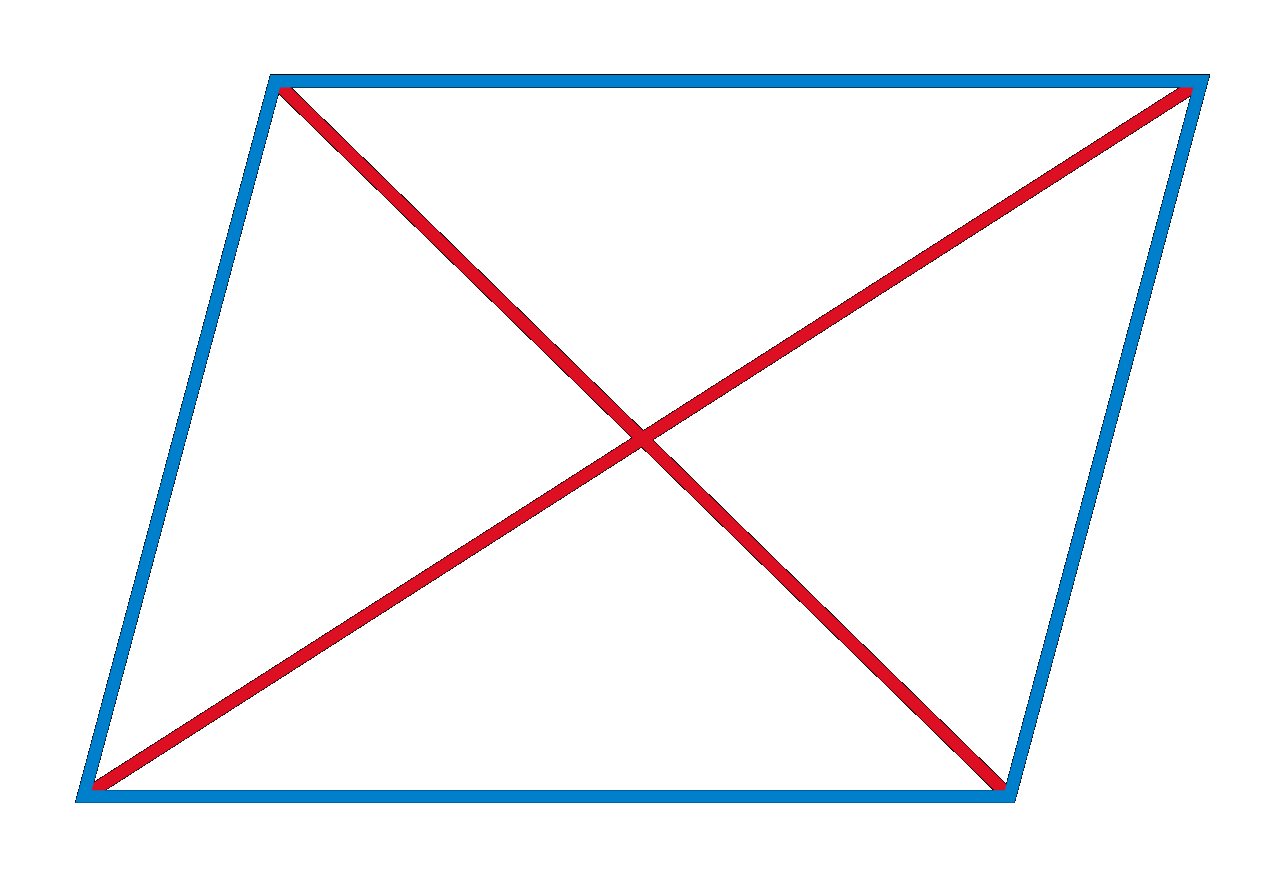
\includegraphics[width=7cm]{parralelogramLaw}
\end{figure}

\begin{Proof}
\begin{align*}
	\|x+y\|^2 + \|x-y\|^2 &= \langle x+y, x+y \rangle + \langle x-y, x-y \rangle\\
	&= 2\langle x,x \rangle +  \langle x,y \rangle -  \langle x,y \rangle + \langle y,x \rangle - \langle y,x \rangle + 2\langle y,y \rangle\\
	&= 2\langle x,x \rangle + 2\langle y,y \rangle\\
	&= 2\|x\|^2 + 2\|y\|^2
\end{align*}
\end{Proof}

It turns out that a norm satisfying the parralelogram law will in fact define an inner product. This shows how norms
define geometries that are more general than euclidean:

\begin{example}{Exploring Parralelogram Law}{exploringParralelogramLawEx}
	\begin{enumerate}
		\item (The polarization Identity) For any $x,y \in \EH$,
			\[
				\langle x,y \rangle = \frac{1}{4}(\|x+y\|^2 - \|x-y\|^2 + i\|x+iy\|^2 - i\|x-iy\|^2)
			\]
			\begin{proof}
				This is simply a matter of computation:
				\begin{align*}
					&\quad \frac{1}{4}(\|x+y\|^2 - \|x-y\|^2 + i\|x+iy\|^2 - i\|x-iy\|^2)\\
					&= \frac{1}{4}(\langle x+y, x+y\rangle - \langle x-y, x-y\rangle + i\langle x + iy\rangle - i\langle x - iy, x- iy\rangle)\\
					&= \frac{1}{4}(\langle x, x\rangle + \langle x,y\rangle + \langle y,x\rangle + \langle
					y,y\rangle - (\langle x, x\rangle - \langle x,y\rangle - \langle y,x\rangle + \langle y,y\rangle)\\
					&\quad +  i(\langle x, x\rangle + \langle x,iy\rangle + \langle iy,x\rangle + \langle
					iy,iy\rangle - (\langle x, x\rangle - \langle x,iy\rangle - \langle iy,x\rangle + \langle
					iy,iy\rangle))\\
					&= \frac{1}{4}( 2\langle x,y\rangle + 2\langle y,x\rangle +  i( 2\langle x,iy\rangle +2 \langle iy,x\rangle))\\
					&= \frac{1}{4}( 2\langle x,y\rangle + 2\langle y,x\rangle +  i(-i)2\langle x,y\rangle +2 ii\langle y,x\rangle)\\
					&= \frac{1}{4}( 2\langle x,y\rangle + 2\langle y,x\rangle +  2\langle x,y\rangle -2 \langle y,x\rangle)\\
					&= \frac{1}{4}4\langle x,y\rangle\\
					&= \langle x,y\rangle
				\end{align*}
			\end{proof}
		\item If $\EH'$ is another Hilbert space, a linear map from $\EH$ to $\EH'$ is unitary if and only if it is
			isometric and surjective
			\begin{proof}
				Let $U$ be unitary so that $\langle Ux, Uy \rangle_2 = \langle x,y \rangle_1$ for any $x,y \in
				\EH$. Letting $x= y$ gives us $\|Ux\|_2 = \|x\|_1$, giving us that it's an isometry. Since $U$ is
				invertible, it is surjective, and so $U$ is a surjective isometry.

				Conversely, let $U$ be a surjective isometry. We need to show its invertible
				(it suffices to show it's injective), an isometry, and that $U$ and $U^{-1}$ are bounded. Clearly,
				$U$ is bounded since $\|U(x)\| \le 1\|x\|$. For injectivity, let $Ux = Uy$, so $Ux - Uy
				= 0$. Taking the norm on both sides, we get:
				\[
					0 = \|0\|_2 = \|Ux - Uy\|_2 = \|U(x-y)\|_2 = \|x-y\|_1
				\]
				where the last equality is due to $U$ being an isometry. Since $\|z\| = 0$ if and only if $z = 0$,
				we have $x-y = 0$, i.e. $x = y$, proving that $U$ is injective. Along with surjectivity, that makes
				$U$ invertible. With this, we can also show that $U^{-1}$ is bounded: for any $y \in \EH'$, there
				exists an $x \in \EH$ such that $U(x) = y$. Thus:
				\[
					\|U^{-1}(y)\| = \|x\| \overset{!}{=} \|U(x)\| = \|y\|
				\]
				where $\overset{!}{=}$ comes from $U$ being an isometry, showing that $\|U^{-1}(y)\| \le 1\cdot \|y\|$, making it also bounded.

				Finally, to show that $\langle Ux, Uy \rangle_2 = \langle x,y \rangle_1$, we will use part (a):
				\begin{align*}
					\langle x,y \rangle &= \frac{1}{4}(\|x+y\|^2 - \|x-y\|^2 + i\|x+iy\|^2 - i\|x-iy\|^2)\\
										&\overset{!}{=} \frac{1}{4}(\|U(x+y)\|^2 - \|U(x-y)\|^2 + i\|U(x+iy)\|^2
					- i\|U(x-iy)\|^2)\\
										&= \frac{1}{4}(\|U(x)+U(y)\|^2 - \|U(x)-U(y)\|^2 + i\|U(x)+iU(y))\|^2
										- i\|U(x)-iU(y)\|^2)\\
										&= \langle U(x), U(y)\rangle
				\end{align*}
				where $\overset{!}{=}$ comes from $U$ being an isometry. Thus:
				\[
					\langle Ux, Uy \rangle = \langle x,y\rangle
				\]
				As we sought to show.
			\end{proof}
	\end{enumerate}
\end{example}

\begin{prop}{Convergence In Inner Product}{convergenceInInnerProd}
	Let $x_n \to x$ and $y_n \to y$. Then $ \langle x_n, y_n \rangle \to \langle x,y \rangle$
\end{prop}

\begin{Proof}
	\begin{align*}
		| \langle x_n, y_n \rangle - \langle x,y \rangle| &= | \langle x_n - x, y_n \rangle + \langle x, y_n
		-y \rangle|\\
		&= \|x_n - x\|\|y_n\| + \|x\|\|y_n\|
	\end{align*}
	which tends to zero since $x_n, y_n \to 0$.
\end{Proof}

When it comes to the right notion of morphism for Hilbert spaces, this is actually not as straight forward as it may
seem. To start with a special case, it is straightforward to imagine an isomorphism:

\begin{defn}{Unitary Map}{unitaryMap}
Let $\EH_1$ and $\EH_2$ be two hilbert spaces with inner products $\langle \cdot, \cdot \rangle_1$ and $\langle
\cdot, \cdot \rangle_2$, and let $U: \EH_1 \rw \EH_2$. Then $U$ is called a \emph{unitary map} if if it is an
invertible linear map that perserves inner products:
\[
	\langle Ux, Uy \rangle_2 = \langle x,y\rangle_1
\]
\end{defn}

The appropriate notion of a morphism that matches this is not so easy. We may result to the fact that all
Hilbert spaces are banach spaces and use continuous linear operators, however such operators do not capture the inner
product structure (it cannot be recovered using this information). There is a way to recover this information if we
instead upgrade our category with an involution, this is known as a dagger category:
\[
	(-)^\dagger: \Hom(a,b) \to \Hom(b,a)
\]
this is a morphism between homsets that satisfy certain propertie given by adjoint (which we'll see in the next
section). Then we recover an inner product and unitary maps. We won't go down the road of looking at dagger categories,
but it is insightful to think about what information is useful in these categories.

Note that by taking $x = y$, we get that $\|x\|_1 = \|Ux\|_2$, i.e. it is an isometry. In fact, the converse is true
too: every surjective isometry is unitary. We can define the operator norm on $\|T\|$ differently using the inner
product:
\[
	\|T\| = \sup_{\|x\| = 1,\ \|y\| = 1} |\langle T(x), y\rangle|
\]
the two are shown to be equivalent whith not too much work:
\begin{proof}
	For $\ge$, using Cauchy-Swartz we get:
	\[
		\sup_{\|x\| = 1,\ \|y\| = 1} |\langle T(x), y\rangle| \le \|T(x)\| \le \|T\|
	\]
	For the other direction
	\begin{align*}
		\|T\| &= \sup_{\|x\| = 1} \|T(x)\|\\
			  &= \sup_{\|x\| = 1,\ T(x) \ne 0} \frac{\langle T(x), T(x)\rangle}{\|T(x)\|}\\
			  &\le \sup_{\|x\| = \|y\| = 1} |\langle T(x), y\rangle|
	\end{align*}
\end{proof}

\subsection*{Subspaces}

Just like for Banach spaces, close spaces of hilbert spaces are hilbert spaces. As we saw in
section~\ref{sec:banDualSp}, we often want to separate an operator by how it \emph{annihilates} a subspace. For Hilbert
spaces, such subspaces are really easy to find:

\begin{defn}{Orthogonal}{orthogonal}
We say that $x$ is \emph{orthogonal} to $y$ if $ \langle x,y \rangle = 0$. We will write $x \perp y$
\end{defn}

If two vectors are orthogonal, the triangle inequality becomes instant:

\begin{thm}{Pythagoras}{pythagoras}
\[
	x\perp y \Rw \|x+y\|^2 = \|x\|^2 + \|y\|^2
\]
\end{thm}

\begin{Proof}
\[
	\|x+y\|^2 = \langle x+y, x+y\rangle = \|x\|^2 + \|y\|^2
\]
\end{Proof}


We might wonder if we take $E \sse H$, can we find all vectors in $H$ that are somehow ``dual'' to $E$? Define it's \emph{orthogonal compliment} to be:
\[
E^\perp = \set{x \in H}{\langle x,y \rangle = 0\ \forall y \in E }
\]
Notice that $E$ is \emph{always} a closed subspace:

\begin{proof}
The fact it's a subspace follows from linearity of the second component.t

for closed, suppose there is a sequecne $\{x_n\} \sse E^\perp$ where $x_n \rw x \in H$. Then:
\[
	|\langle x,y\rangle| \le |\langle x-x_n, y\rangle| \le \|x-x_n\|\|y\| \rw 0 \quad \text{as $n \rw \infty$}
\]
\end{proof}

We can also find closed (and not closed) subspace of hilbert spaces:

\begin{example}{Subspaces Examples}{subspacesExamplesEx}
\begin{enumerate}
	\item If $\EH$ is a finite-dimensional Hilbert space, then all subspace are closed
	\item If $\EH$ is infinite-dimensional, consider $\EH = L^1([0,1])$ with the $L^2$ inner product. and take
		$P([0,1]) \sse L^1([0,1])$ to be the subspace of all polynomial functions. This is is certainly not equal to
		$L^1([0,1])$, however polynomial functions are dense in $L^1([0,1])$ (they can arbitraily approximate
		continuous bump characteristic functions, and hence simple functions). However, their closure is
		$L^1([0,1])$, showing that $P([0,1])$ cannot be closed.
	\item Assume $E \sse \EH$ is an open subspace. Then since $0 \in E$, there exists a $r > 0$ such that
		\[
			B_r(0) \sse E
		\]
		However, for any nonzero element $x \in \EH$,
		\[
			\frac{r}{2\|x\|}x \in B_r(0) \sse E
		\]
		Since $E$ is closed under scalar multiplication, this shows that $x \in E$, so $\EH \sse E$, so $\EH = E$,
		showing that the only open subspace of $\EH$ is $\EH$ itself.
\end{enumerate}
\end{example}

Thus, we are interested in closed subspace since are closed under limits, meaning we can use our tools from analysis to
get the following decomposition result:

\begin{thm}{Hilbert Space Decomposition}{hilbertSpDecomp}
Let $E \sse \EH$ be a closed subspace. Then:
\[
	\EH = E\oplus E^\perp
\]
In particular, for any $ x\in H$, there is a unique $y\in E$ and $z \in E^\perp$ such that $x = y + z$.
\end{thm}

\begin{Proof}
Let $x \in \EH$, and let $\delta = \inf\set{ \|x-y\| = \rho(x,y)}{y \in E}$ (which exists by completeness of $\R^n$
and $\EH$). let $\{y_n\} \sse E$ be a sequence such that $\|x - y_n\| \rw \delta$. We will show that $\{y_n\}$ is
a cauchy sequence, and then find a limit point for it. By the parralelogram law:
\[
	2(\|x - y_n\| + \|x - y_m\|) = \|y_n - y_m\|^2 + \|(y_n + y_n) - 2x\|^2
\]
Since $y_n + y_m \in E$, for sufficinetly large $N$ so that $n,m > N$:
\begin{align*}
	\|y_n - y_m\|^2 &= 2\|y_n - x\|^2 + 2\|y_m - x\|^2 - 4\|\frac{1}{2}(y_n + y_n) - x\|^2\\
					&\le2\|y_n - x\|^2 + 2\|y_m - x\|^2 - 4\delta^2\\
\end{align*}
and as $n,m \rw \infty$, this sequence goes to $4\delta^2 - 4\delta^2 = 0$, and so $\|y_n - y_m\| \rho(y_n, y_m) \rw
0$, meaning $\{y_i\}_i$ is a cauchy sequence. Take $y \lim y_n$. Then since $E$ is closed, $y \in E$. By
construction $\|x-y\| = \delta$. Now let $z = x-y$.

I claim that $z \in E^{\perp}$, that is $\langle z,u \rangle = 0$ for all $u \in E$. So, consider $\langle u,z
\rangle$ for any $u \in E$. If $ \langle u,z \rangle$ is complex, multiply it by a [complex] unit-length scalar to make
it real ($\langle u,z \rangle = 0$ if and only if $a \langle u,z \rangle = 0$). With the fact that it's real, we
will do a sneaky trick where we take advantage of optimization of differentiable functions. In particular, let
\[
	f: \R \rw \R \quad f(t) = \|z + tu\|^2 = \|z\|^2 + 2t \langle z,u \rangle + \|u\|^2
\]
$f$ is certainly a differentiable function, being a polynomial with a square-root on $\R$. Furthermore, $z = x-y$ is
the minimal value of $\|x-y\|$, and so the minimal value of $\|x-y\|^2$. It follows that $z + ut$ is not minimal,
and so this equation is has a minimum when $t = 0$. Thus, we get $0 = f'(0) = 2 \langle u,z \rangle$, implying that
$ \langle u,z \rangle = 0$. Since $u$ was arbitrary, we get that $z \in E^\perp$.

To show that $z$ is the minimal distance from $x$, let's say there was another $z' \in E^\perp$ that satisfied the
equation. Then by the Pythagorean theorem:
\begin{align*}
	\|x-z'\| &= \|(x-z)+(z-z')\|^2\\
			 &= \|x-z\|^2 +\|z-z'\|^2 &x-y \in E, z-z' \in E^\perp\\
			 &\ge \|x-z\|^2
\end{align*}
So equality holds if and only if $z = z'$, meaning $z$ is of minimal distance to $x$. A similar reasoning shows the
same for $y$.

To show uniqueness, let's say $y + z = x = y' + z'$. Then $y - y' = z-z' \in E\cap E^\perp = \{0\}$, so $y-y' = z-z'
= 0$, which can be used to show that $y = y'$ and $z = z'$, completing the proof.
\end{Proof}

\begin{cor}{Double Dual Property}{doubleDualProperty}
	For each subset $Y \sse H$, the smallest closed subspace of $H$ containing $Y$ is $(Y^\perp)^\perp$. In
	particular, if $Y$ is a subspace of $H$, then $\oln{X} = (X^\perp)^\perp$
\end{cor}

\begin{Proof}
	exercise
\end{Proof}


We said that orthogonal vector are somehow dual to each other. However, there is the more classical notion of ``dual''
vector spaces. Let $\EH^*$ be set of all linear functions from $\EH$ to the underlying field (usually $\C$, but
sometimes $\R$); such linear functions are called functionals. It turns out that all linear functionals can be written
in the form $f_y(x) = \langle x,y \rangle$, and we can define a norm on $\H^*$ such that $\|f_y\| = \|y\|$. Thus, $y
\mapsto f_y$ will define a conjugate-linear isometry from $\EH$ to $\EH^*$. The following theorem shows tha this map is
surjective:

\begin{thm}{Natural Isomorphism To $\EH^*$ (Riesz Representation)}{naturalIsoTolinearFunctionals}
Let $f \in \EH^*$. Then there exists a $y \in \EH$ such that $f(x) = \langle x,y \rangle$ for all $x \in X$.
\end{thm}

\begin{Proof}
	It easy easy to check uniqueness: if $ \langle x,y \rangle = \langle x,y' \rangle$ for all $x$, then let $x = y-y'$.
	Manipulating the equation, we get that $\|y - y'\| = 0$, so $y = y'$.

	If $f$ is the zero functional, then take $y = 0$. If otherwise, then let $\EM = \set{x}{f(x) = 0}$ be the kernel of
	$f$. It is clearly a subspace, and any squence will also necesarily converge within $\EM$, and so it is also closed.
	Furthermore, $\EM$ is a proper subspace, since $f \ne 0$. Thus, $\EM^\perp \ne \{0\}$ by the previous proof.

	Now, pick any $z \in \EM^{\perp}$ with $\|z\|  =1$. Then if we set $u = f(x)z - f(z)x$, we have that $u \in \EM$.
	Hence:
	\[
		0 = \langle u,z \rangle = f(x)\|z\|^2 - f(z)\langle x,z\rangle = f(x) - \langle x, \oln{f(z)}z\rangle
	\]
	re-arrangine and setting $y = \oln{f(z)}z$, we get
	\[
		f(x) = \langle y,z \rangle
	\]
	as we sought to show.
\end{Proof}

The uniqueness makes this map to be injective, and by linearity of $f$ and the first component of the inner product
makes it is an isomorphism. Furthermore, since $\|f_y\| = \|y\|$, limits are also preserved, and so this in fact defines
an isomorphism between $\EH \cong \EH^*$. Notice how this differs from vector-spaces where there is no natural
isomorphism between $V$ and $V^{*}$ (there is one between $V$ and $V^{**}$).

As we've done with banach spaces, we should define the topology on the dual of $H$. By the Riesz representation
theorem, we see that any $f \in H^*$ is simply $\langle \cdot, y\rangle$ for appropriate $y \in H$. Hence, the weak
topology on $H$ is the initial topology corresponding to the functionals $x \mapsto \langle x, y\rangle$.


Note that it is important that the space is \emph{complete}. The following shows what can happen otherwise:
\begin{example}{Functional Without Riesz Representation}{funcalWithoutRieszRepEx}
	Let $V= \C[x]$ where we treat any $f \in \C[x]$ as a function $f: [0,1] \to \C$. Then:
	\[
		\langle f,g \rangle = \int_0^1 f(t)\oln{g}(t)dt
	\]
	Note that $V$ is not complete: Letting $V \sse C([0,1])$ we see there is a Cauchy sequence in $V$ that converges to
	$|x-0.5|$ in $C([0,1])$. Let's say that Riesz Representation theorem still holds, so that for $L_z \in V^*$ where
	$L(f) = f(z)$, there exists a $g \in V$ such that
	\[
		L(f) = \langle f,g \rangle = \int_0^1 f(t)\oln{g}(t)dt
	\]
	Then
	\[
		f(z)  =\int_0^1 f(t)\oln{g}(t)dt
	\]
	For any $f \in V$. Define $h(z) = x-z$ so that $hf \in V$ and $(hf)(z) = h(z)f(z) = 0$. Hence:
	\[
		0 = \int_0^1 h(t)f(t)\oln{g(t)}dt
	\]
	If $f = \oln{h}g \in V$ then
	\[
		0 = \int_0^1 |h(t)|^2||g(t)|^2dt
	\]
	since $h \ne 0$, it must be that $g = 0$ a.e. But then $ \langle f,g \rangle = 0$ a.e., so $L_z(f) = 0$ almost
	everywhere. But that's a contradiction, as certianly $L_z$ is not $0$ a.e.
\end{example}

However, notice that if we take the completion, we will have enough elements so that $L_z$ does indeed have a Riesz
Representation.

\subsection*{Orthogonal Basis}


In this section, we will show how Hilbert spaces have much nicer dense sets than Banach spaces. In particular, we shall
see that we will be able to upgrade the notion of a basis more readily to Hilbert spaces. Since we are studying infinite
dimensional vector-spaces, we often care more about ``countable linear combination'' rather than ``finite linear
combination'' as we have for vector-spaces. To distinguish the two, we will call \emph{Hamel basis} a set of linearly
independent elements for which all \emph{finite linear combinations} can represent every element of the vector space. We
will call a \emph{Schauder basis} a set of linearly independent elements for which all \emph{countable inear
combinations} can represent every element of the vector space. If every element in a Schauder basis has norm $1$ and is
orthogonal, we call it an \emph{orthonormal basis}. Since we have an inner-product that is complete, it would be nicest
if this vector-space has an orthonormal basis. We strive to this end in the following build-up:

\begin{thm}{Bessel's Inequality}{besselInequality}
If $\{u_\alpha\}_{\alpha \in A}$ is an orthonormal set in $\EH$, then for any $x \in \EH$:
\[
	\sum_{\alpha \in A} | \langle x, u_\alpha\rangle|^2 \le \|x\|^2
\]
As a consequence, $\set{\alpha}{ \langle x, u_\alpha \rangle \ne 0 }$ is countable.
\end{thm}

\begin{Proof}
It suffices to show that $\sum_{\alpha \in F} | \langle x, u_\alpha \rangle|^2 \le \|x\|^2$ for any finite subset $F
\sse A$, since if it fails for some countable amount, it will fail for some finite amount. Then we see that:
\begin{align*}
	0 &\le \left\|x - \sum_{\alpha \in F} \langle x, u_\alpha\rangle u_\alpha\right\|\\
	  &=  \|x\|^2 - 2\Re\left\langle x , \sum_{\alpha \in F} \langle x, u_\alpha\rangle u_\alpha\right\rangle + \left\|
	  \sum_{\alpha \in F} \langle x, u_\alpha\rangle u_\alpha\right\|\\
	  &= \|x\|^2 - 2\sum_{\alpha \in F}|\langle x, u_\alpha\rangle|^2 + \sum_{\alpha \in F} |\langle x,
	u_\alpha\rangle|^2 &\text{Pythagorean Theorem}\\
	  &= \|x\|^2 - \sum_{\alpha \in F} |\langle x, u_\alpha\rangle|^2
\end{align*}
and manipulating the final equation we get:
\[
	   \sum_{\alpha \in F} |\langle x, u_\alpha\rangle|^2 \le \|x\|^2
\]
as we sought to show
\end{Proof}

This in particular is important for uncountable sets. In the following we establish when equality holds, and thus when
an orthonormal set is an orthonormal basis

\begin{thm}{Orthonormal Basis Condition}{orthonormalBasisCond}
Let $\{u_\alpha\}_{\alpha \in A}$ be an orthonormal set in $\EH$. Then the following are equivlent:
\begin{enumerate}
	\item (Completenss) If $\langle x, u_\alpha \rangle = 0$ for all $\alpha$, then $x = 0$
	\item (Parseval's Identity) $\|x\|^2 = \sum_{\alpha \in A} |\langle x, u_\alpha \rangle|^2$ for al l$x \in \EH$
	\item For each $x \in \EH$, $x = \sum_{\alpha \in A} \langle x, u_\alpha \rangle u_\alpha$ where the right hand
		side sum has only countably many nonzero terms and converges in the norm topology no matter the order of the
		terms (so converges absolutely?)
\end{enumerate}
\end{thm}

\begin{Proof}
p.175 Folland
\end{Proof}

\begin{defn}{Orthonormal Basis}{orthonormalBasis}
Let $\{u_\alpha\}_{\alpha \in A}$ be an orthonormal set. Then if the set satisfies any of the 3 conditions in
theorem~\ref{th:orthonormalBasisCond}, it is called an \emph{orthonormal basis}.
\end{defn}


\begin{thm}{Hilbert Space Basis}{hilbertSpBasis}
Every Hilbert space has a basis
\end{thm}

\begin{Proof}
Application of Zorn's lemma: The collection of ordered orthonormal sets ordered by inclusion has a maximal element,
and maximality is equivalent to the first property of theorem~\ref{th:orthonormalBasisCond}.
\end{Proof}

Now that we have established a basis for Hilbert spaces, we will seperate them into 3 categories: Those with finite,
countable, and uncountable basis. In most cases, we will be working with countable basis due to the following property:

\begin{prop}{Seperable Hilbert Spaces}{seperableHilbertSps}
A Hilbert space $\EH$ is seperable if and only if it has a countable orthonormal basis, in which case every
orthonormal basis for $\EH$ is countable.
\end{prop}

Here, we are using the word seperable to mean countable dense subset.

\begin{Proof}
p. 176
\end{Proof}

 With the definition of an isomorphism, we can see that all Hilbert spaces are
isomorphic to $\ell^2(A)$ given basis $A$:

\begin{thm}{Classifying Hilbert Spaces}{classifyingHilbertSps}
Let $\{e_\alpha\}_{\alpha \in A}$ be an orthonormal basis for $\EH$. Then the correspondence
\[
	x \mapsto \hat{x} \qquad \hat{x}(\alpha) = \langle x, u_\alpha \rangle
\]
is a unitary map from $\EH$ to $\ell^2(A)$.
\end{thm}

\begin{Proof}
	We'll show it's a surjective isometry, which is equivalent to it being unitary.

	First off, the map $x \rw \hat{x}$ is linear since the inner product is linear in each component, and it is an
	isometry by Parseval identity: $\|x\|^2 = \sum |\hat{x}(x)|^2$.

	For surjectivity, let $f \in \ell^2(A)$, so $\sum_{\alpha \in A} |f(\alpha)^2| < \infty$, so the Pythagorean shows
	that all partial sumns of the series $\sum f(\alpha)u_\alpha$ are Cauchy \footnote{Note that only countably many
	terms are nonzero}, so $x = \sum_\alpha f(\alpha)u_\alpha$ exists in $\EH$ and $\hat{x} = f$.
\end{Proof}



\section{Operators on Hilbert Spaces}

In this section, we try to generalize many notion's we've seen before, including:
\begin{enumerate}
	\item adjoints, self-adjoint, and normal operators
	\item sign and absolute value and when can we decompose a function into this form
	\item diagonalizable
	\item polar decomposition (think of how for every $z \in \C$, $z = \arg(z)|z|$)
\end{enumerate}

\subsection*{Adjoints}

Hilbert spaces have very simple dual structure, since $\H \cong \H^*$ in a very natural way with the inner product of
$\H$. Thus, the problem of finding the structure of dual spaces is fully finished for hilbert spaces. Due to this very
simple dual structure, we will be able to properly define an ``opposite'' operator given any operator $T: \H_1 \to
\H_2$. In essense, there is an interesting symmetry in the structure of any map: Given a map $T: \H_1 \to \H_2$ between
two hilbert spaces, there is a natural dual map $T^*: \H_{2}^* \to \H_1^*$. Hence, we have
\[
	(-)^*: \Hom(\H_1, \H_2) \to \Hom(\H_2^*, \H_1^*)
\]
and since in Hilbert spaces $\H_i\cong \H_i^*$, we may envision this map as ``flipping'' the direction of arrows in
a natural way:
\[
	(-)^*: \Hom(\H_1, \H_2) \to \Hom(\H_2, \H_1)
\]
Not only does this map exist, but it is an isometric isomrophism (in \bf{Ban})! We will start with the special case of
$\Hom(\H, k) = \H^*$. We will find that $(-)^*$ is a map
\[
	(-)^*: \Hom(\H, \H) \to \Hom(\H, \H)
\]
The following shows how we can define such a dual
and some consequences:

\begin{lem}{Endomorphism and And Inner Products}{DualAndInnerProds}
	Let $\H$ be a complex hilbert space. Then there is a bijective isometric correspondence between
	$\End_k(\H)$ and bounded sesquilinear forms on $\H$ given by tne map $T \to B_T$ where
	\[
		B_T(x,y) = \langle x, T(y)\rangle
	\]
\end{lem}

\begin{Proof}
	Let $T \in \End_k(\H)$. Then certainly $B_T$ is a sequilinear form on $\H$ bounded by $\|T\|$ since
	\begin{align*}
		\|B_T\| &= \sup\set{|B_T(x,y)|}{\|x\| \le 1,\ \|y\|\le 1}\\
				&= \sup\set{|\langle x, T(y)\rangle|}{\|x\|\le 1,\| y \| \le 1 }\\
				&\le \|T\|
	\end{align*}
	On the other hand
	\begin{align*}
		\|T(x)\|^2 &=  \langle T(x), T(x)\rangle\\
		&= B_T(T(x), x)\\
		&\le \|B_T\|\|T(x)\|\|x\|\\
		&\le \|B_T\|\|T\|\|x\|^2
	\end{align*}
	showing that $\|T\| \le \|B_T\|$, and so $\|T\| = \|B_T\|$.
\end{Proof}

\begin{thm}{Existence Of Adjoint}{existenceAdjoint}
	Let $T \in \End_k(\H)$. Then there exists a unique $T^*$ in $\End_k(\H)$ such that
	\[
		\langle T(x), y\rangle = \langle x, T^*(y)\rangle
	\]
	for all $x,y \in \H$. The map $T \mapsto T^*$ is conjugate linear, contravariant with respect to
	multiplication, an isometry of $\End_k(\H)$ onto itself, an involution, and satisfies
	\[
		\|T^*T\| = \|T\|^2
	\]
\end{thm}

\begin{Proof}
	Fix $T \in \End_k(\H)$, and let $B_T(x,y)$ be a continuous sesquilinear form defined as $(x,y) \mapsto \langle T(x), y
	\rangle$. Then by lemma~\ref{lm:DualAndInnerProds}, there exists a $T^* \in \End_k(\H)$ such that $T^* \to B_T$. In
	particular
	\[
		B_T(x,y) = \langle x, T^*(y) \rangle
	\]
	Thus,
	\[
		\langle T(x), y\rangle = \langle x, T^*(y)\rangle
	\]
	giving us existence of such an operator. We now establish all the properties named in the theorem. By conjugate
	symmetry
	\begin{align*}
		\langle x, T^{**}(y)\rangle &= \langle T^*(x), y\rangle\\
			&= \oln{\langle y, T^*(x)\rangle}\\
			&= \oln{\langle T(y), x\rangle}\\
			&= \langle x, T(y)\rangle
	\end{align*}
	Thus, $T^{**}$ and $T$ correspond to the same sesquilienar form, thus $T^{**} = T$. This also shows that
	$T\mapsto T^{*}$ is an involution. Furthermore:
	\[
		\langle x (ST)^*y\rangle = \langle S(T(x)), y\rangle = \langle T(x), S^*(y)\rangle = \langle x,
		T^*(S^*(y))\rangle
	\]
	thus $(S\circ T)^* = T^*\circ S^*$ showing $(-)^*$ is a contravariant endofunctor. Since the operator norm
	is submiltiplicative, we have $\|T^*T\| \le \|T\|\|T^*\|$. On the other hand, applying $\angle T(x), y\rangle
	= \langle x, T^*(y)\rangle$ to $T^*$ we get
	\[
		\|T(x)\|^2 = \langle T(x), T(x)\rangle = \langle T^*(T(x)), x\rangle = \|T^*T\|\|x\|^2
	\]
	showing that $\|T\|^2 \le \|T^*T\\$. Combining these we get $\|T\|\le \|T^*\|$, hence $\|T\| = \|T^*\|$ (since
	$T^{**} = T$). This finishes the proof.
\end{Proof}

Note that if $\H$ is a finite dimensional complex Hilbert space, then each operator $T$ has a matrix representation, say
$(\alpha_{ij)})$. Then $T^* = (\oln{\alpha_{ji}})$, i.e. $T^* = \oln{T^t}$ where $T^t$ is the transpose given the matrix
representation.

\begin{defn}{Adjoint And Self-Adjoint}{adjointAndSelf-Adjoint}
	Let $T \in B(\H)$ be a continuous linear operator between Hilbert spaces. Then $T^*$ is called the
	\emph{adjoint} of $T$. If $T = T^*$, then $T$ is said to be \emph{self adjoint} (or \emph{Hermitian}).
\end{defn}

\begin{prop}{Adjoint Properties I}{adjointPropI}
	Let $T \in \End_k(\H)$. Then
	\[
		\ker(T^*) = (T(\H))^\perp
	\]
\end{prop}

\begin{Proof}
	Since $ \langle T(x), y \rangle = \langle x, T^*(y) \rangle$ we have $y \in \ker(T^*)$ when $y \in
	(T(\H))^\perp$. Conversely, if $y \in (T(\H))^\perp$, then $T^*(y) \in \H^\perp = \left\{ 0 \right\}$.
\end{Proof}

For ease of reference, we shall list some of the results we have proven in the theorem:
\begin{prop}{Adjoint Properties II}{adjointPropII}
	Let $T,S \in B(\H)$. Then:
	\begin{enumerate}
		\item $(T+S)^* = T^*+S^*$
		\item $(cT)^* = \oln{c}T^*$
		\item $(TS)^* = S^*T^*$
		\item $(T^*)^* = T$
		\item $I^* = I$
	\end{enumerate}
\end{prop}

\begin{Proof}
	If you're not convinced of any of these, double check the theorem or try proving it again.
\end{Proof}

\begin{prop}{Adjoint Properties III}{adjointPropIII}
	Let $T \in \End_k(\H)$. Then the following are equivalent:
	\begin{enumerate}
		\item $T$ is invertible (so $T^{-1} \in \End_k(\H)$)
		\item $T^*$ is invertible
		\item $T$ and $T^*$ are bounded away from zero.
		\item $T$ and $T^*$ are injective, and $T(\H)$ is closed
		\item $T$ is injective and $T(\H) = \H$
	\end{enumerate}
\end{prop}

\begin{Proof}
	Since $T$ is invertible, $T^{-1}T = TT^{-1} = I$, and so $(T^{-1})^*$ is the inverse of $T^*$, giving $(1)
	\LRw (2)$.

	For $(1) \Rw (3)$, we say that an operator $F$ is bounded away from zero if
	\[
		\|x\| \le C\|F(x)\|
	\]
	for some constant $C$. In our case:
	\[
		\|x\| = \|T^{-1}\circ T(x)\| \le \|T^{-1}\|\|T(x)\|
	\]
	Since $(1) \LRw (2)$, the same holds for $T^*$.

	For $(3) \Rw (4)$, We have $\|T(x)\| \ge \epsilon\|x\|$ and $\|T^*(x)\| \ge \epsilon\|x\|$ for some $\epsilon
	> 0$ and all $x \in \H$. Thus certainly both $T$ and $T^*$ are injective: if $T(x) = T(y)$ then
	\[
		0 =\|T(x) - T(y)\| =\|T(x-y)\| \ge \epsilon\|x-y\|
	\]
	hence $\|x-y\| = 0$, so $x = y$. Furthermore, $\|T(x) - T(y)\| \ge \|x-y\|$ imples that $T(\H)$ is
	complete, hence a closed subspace of $\H$.

	For $(4) \Rw (5)$, by corollary~\ref{co:doubleDualProperty} ($\oln{Y} = (Y^\perp)^\perp$) and
	proposition~\ref{pr:adjointPropI} we get
	\[
		\oln{T(\H)} = (T(\H)^\perp)^\perp = (\ker(T^*))^\perp = \{0\}^\perp = \H
	\]
	where the last equality come from $T^*$ bein injective.

	Finally, for $(5) \to (1)$, we use the open mapping theorem.
\end{Proof}

This allows us to generlize this result to the followin
\begin{prop}{Inversing Maps}{inversingMaps}
	 Let $\H_1$ and $\H_2$ be hilbert spaces and consider an operator $T \in \Hom_k(\H_1, \H_2)$. Then
		there exists a unique operator $T^* \in B(\H_2, \H_1)$ such that
		\[
			 \langle T(x), y \rangle = \langle x, T^*(y) \rangle
		 \]
		 show that the map $T \to T^*$ is conjugate linear isometry of $\Hom_k(\H_1, \H_2)$ to
		 $\Hom_k(\H_2, \H_1)$ and satisfies
		 \[
			 \|T^*T\| = \|T\\^2 = \|TT^*\|
		 \]
\end{prop}

\begin{Proof}
	 Let
	 \[
		\hat{T} =
	 \begin{pmatrix}
		 0 & 0\\
		 T & 0
	 \end{pmatrix} \in \End_k(\H_1\oplus \H_2)
	 \]
	 By theorem~\ref{th:existenceAdjoint}, there is a unique function $\hat{T}^*$ such that
	 \[
	 	\langle \widehat{T}(x_1, x_2), (y_1, y_2) \rangle = \langle (x_1, x_2), \widehat{T}^*(y_1, y_2) \rangle
	 \]
	 By definition of
	 $\widehat{T}$, we see
	 \[
		 \widehat{T}^* = \begin{pmatrix}
			 0& T^*\\
			0 & 0
		 \end{pmatrix}
	 \]
	 Hence we have that $T^*$ is a function with domain and codomain $T^*: \H_2 \to \H_1$. It
	 follows that
	 \[
		 \langle T(x), y \rangle = \langle x, T^*(y) \rangle
	 \]
	 and by theorem~\ref{th:existenceAdjoint}, $T$ and $T^*$ respect all the desired properties, completing the proof.
\end{Proof}

For the rest of this seciton, we will focus on $T \in B(\H)$ insead of $T \in B(\H_1, \H_2)$. The reason for this is to
find suitable decompositino theorems of $T$ generlizing the notion of eigenvalues.

Recall that over finite dimensional vector spaces, $TT^* = T^*T$ implied $T$ was diagonalizable, with the usual special case of $T = T^*$
(self-adjoint) being looked into. We would like to know if this notion of diagonalizability for normal operators remains
true for infinite dimensional Hilbert spaces. We shall see that this is not the case, some more conditions is required
(for ex. a special case of digaonalizable operators will be comapct normal operators). Before we get into the
technicalities, I want to put a word on how I think about $TT^* = T^*T$. In my mind, when two functions commute, it
means that one function is somehow ``invariant'' with respect to the other. Think of PDE's with equations that commute
with the differential operator that makes it invariant to the Lorenzian metric. In this case, I like to think of $T$
being somehow ``symmetric''. Since $TT^*(x) = T^*T(x)$ for all $x \in \H$, and $T^*$ is in some ways the dual (think of
ref:HERE, the generalization), we see that $T$ is ``invariant'' to the effect of the dual $T^*$. We shall see in
a moment that the invariant to the dual is translated to $T$ and $T^*$ being metrically identical. In the simpleset case
of $T = T^*$, it is evident why this is the case. If $T = T^*$, we can deepen our intuition with complex numbers: if we
consider $T: \C \to \C$ where $T(z) = z$, then $T^*(z) = \oln{z}$. Hence, $T = T^*$ if and only if $T(\C) \sse \R$,
since only the real number are invariant under conjugation.

\begin{defn}{Normal Operator}{normalOperator}
	Let $T \in \End_k(\H)$. Then $T$ is said to be \emph{normal} if it commutes with its adjoint, i.e. if $T^*T
	=TT^*$
\end{defn}

As an immedaite consequence, we have
\[
	\|T(x)\| = \langle T^*\circ T(x), x \rangle^{1/2} = \langle T\circ T^*(x), x \rangle^{1/2} = \|T^*x\|
\]
showing that $T$ and $T^*$ are metrically identical. In fact, by the palalalogram law (also known as polarization
identity) if $T \in \End_k(\H)$ such that $T$ and $T^*$ ar emetrically identical, we can show $ \langle T^*\circ T(x),
y \rangle = \langle T\circ T^*(x), y\rangle$ for all $x,y$ and so $T$ is normal by lemma~\ref{lm:DualAndInnerProds}. By
proposition~\ref{pr:adjointPropIII}, an operator is normal if and only if it is bounded away from zero.

\subsection*{Positive Operators}

\begin{defn}{Positive Operator}{positiveOperator}
	Let $T \in \End_k(\H)$. Then $T$ is said to be \emph{positive} if $T = T^*$ and $ \langle T(x),
	x \rangle \ge 0$ for all $x \in \H$. If $k = \C$, the positivey condition implies self-adjointness by the
	polarization identity.
\end{defn}

Certainly, the sum of two positive operators is positive (geometrically, positive operatros form a cone in
$\End_k(\H)$). However the product is not positive, and need not be self-adjoint.




\begin{example}{Positive And Non-Positive Operators}{positiveAndNon-PositiveOperatorsEx}
	here

	However, if the opeartors commute (if the product is self-adjoint), we see that there is a product that is
	positive since $(ST = S^{1/2}TS^{1/2} \ge 0$ by what we'll show in the next proposition)
\end{example}

Let $B(\H)_{sa} \sse \End_\R(\H)$ be the collection of self-adjoint operators. Then  this is a closed subspace,
this subspace intersected with the conte of positive operators defines an ordder $S \le T$ if $T-S \ge 0$. By taking
the case of 2 dimensional real subspaces and $\End_\R(\R^2)$, this order is not total, not even a lattice order.

We
require the following lemma to gain some important results (which will be an immedate consequence of the spectral
theorem in ref:HERE)

\begin{lem}{Square Root Lemma}{squareRootLemma}
	If $S \le T$ in $B(\H)_{sa}$, then $A^*SA \le A^*TA$ for every $A \in \End_k(\H)$. If morever $) \le S$,
	then $\|S\| \le \|T\|$
\end{lem}

\begin{Proof}
	Since $S \le T$, we know that $ \langle (T-S)(y), y \rangle \ge 0$ for evey $y \in \H$. Replacing $y$ with
	$A(x)$ for appropraite $x \in \H$, it follows that $A^*(T-S)A \ge 0$, so $A^*SA \le A^*TA$.

	If $0 \le S \le T$, by the Cauchy-Schwarz inequality on the positive sesquilinear form $\langle S(\cdot),
	\cdot\rangle$, we get that for every pair of unit vectors $x,y \in \H$
	\[
		| \langle S(x) , y\rangle|^2 \le \langle S(x), x) \rangle \langle S(y), y \rangle \le \langle
		T(x), x \rangle \langle T(y), y \rangle \le \|T\|^2
	\]
	Hence, $\|S\|^2 \le \|T\|^2$ by lemma~\ref{lm:DualAndInnerProds}.
\end{Proof}

\begin{lem}{Approximation Lemma}{polyApproximationLemma}
	There is a sequence $(p_n)\sse \R[x]$ of polynomials with positive coefficients such that $\sum p_n$
	converges uniformally on $[0,1]$ to
	\[
		t \mapsto 1 - (1-t)^{1/2}
	\]
\end{lem}

\begin{Proof}
	This is immediate from real analysis, but we can also construct it explicitly.If $q_0 = 0$ and $q_n(t)
	= \frac{1}{2}(t + q_{n-1}(t)^2)$, then we can see that each coefficent of $q_n$ is positive and that $q_n(t)
	\le 1$ for every $t \in [0,1]$. Morever, since
	\[
		2(q_{n+1} - q_n) = q_n^2 - q_{n-1}^2 = (q_n - q_{n-1})(q_n + q_{n-1})
	\]
	it follows by induction that each polynomial $p_n = q_n - q_{n-1}]$ has positive coefficients. Taking the
	$q_n$ as elements of $C([0,1])$, we see they converge pointwise to $[0,1]$ to a function $q$ such that
	$2q(t) = t + q(t)^2$. Thus, $q(t) = 1 - (1-t)^{1/2}$. Sicne $q \in C([0,1])$ and $[0,1]$ is compact, by the
	monotone ocnvergence $q_n \nearrow q$ si in fact uniform by Dini's lemma, hence
	\[
		\sum p_n = \lim q_n = q
	\]
	completing the proof.
\end{Proof}

\begin{prop}{Square-Rooting Positive Operator}{square-RootingPositiveOperator}
	Let $T \in \End_k(\H)$ be a positive operator. Then there is a unique positive operator $T^{1/2}$ such that
	$(T^{1/2})^2 = T$. Moreover, $T^{1/2}$ commutes with every operator commuting with $T$.
\end{prop}

\begin{Proof}
	Analysis Now p.92
\end{Proof}

\begin{prop}{Invertible Positive Operator}{invertiblePositiveOperator}
	A positive operator $T$ is invertible in $\End_k(\H)$ if and only if $T \ge \epsilon I$ for some $\epsilon > 0$.
	I that case, $T{^-1} \ge $ and $T^{1/2}$ is invertib,e and $(T^{-1})^{1/2} = ( T^{ 1/2 })^{-1}$. If $T \le S$,
	then $S^{-1} \le T^{-1}$
\end{prop}

\begin{Proof}
	Analayis now p.94
\end{Proof}

\subsection*{Projection}

Let $W \sse \H$ be a closed subspace of a hilbert space $H$. Then we know that $\H = W + W^\perp$. In particular,
for eah $y \in \H$, we have $y = w + w^\perp$, $w \in W$ and $w^\perp \in W^\perp$. Since
\[
	\alpha y_1 + \beta y_2 = (\alpha x_1 + \beta x_2) + (\alpha x_1^\perp + \beta x_2^\perp)
\]
is the decomposition of a linear combination, it follows that $P: \H \to \H$ given by $P(y) = x$ is an operator in
$\End_k(\H)$ with $\|P\| \le 1$. Note $P$ is idempotent $(P^2 = P$), self-adjoint, and positive since
\[
	 \langle P(y_1), y_2 \rangle = \langle x_1< x_2 + x_2^\perp \rangle = \langle x_1, x_2 \rangle = \langle x_1
	 + x_1^{\perp}, x_2 \rangle = \langle y_1, P(y_2) \rangle
\]
and
\[
    \langle P(y), y \rangle = \langle x, x+x^\perp \rangle = \|x\|^2 \ge 0
\]
\begin{defn}{(Orthogonal) Projection}{(Orthogonal)Projection}
 	The map $P$ in the above is called the \emph{(orthogonal) projection}.
\end{defn}

If $P$ is a self-adjoint and idempotent in $\End_k(\H)$, then
\[
	W = \set{x \in \H}{P(x) = x} = P(\H)
\]
is a closed subsapce of $\H$. If $w^\perp \in W^\perp$, we have (since $P = P^*$) that
\[
	\|P(w^\perp)\|^2 = \langle w^\perp, p^2(w^\perp) \rangle = 0
\]
Thus, $P$ is an orthogonal projection of $\H$ onto $W$. Note that $I-P$ is the projection on $W^\perp$.

Projections are some of the east operators we may construct, and can be thought as the ``characteristic function'' from
real analysis. The analogue of simple function is then obtained by decomposing $\H$ into a finite orthogonal sum
\[
	\H = W_1 \oplus W_2\oplus \cdots \oplus W_n
\]
corresponding to the projections $P_1, ..., P_n$ which are pairwise orthogonal ($P_iP_j = 0$ for $i \ne j$
satisfying $\sum P_i = I$). We may then consider
\[
	T = \sum \lambda_n P_n
\]
for scalars $\lambda_1, \lambda_2, ..., \lambda_n \in k$. This may look familiar to the notion of
\emph{diagonalization}. Indeed, we may generalize the concept to infintie dimensions like so:
\begin{defn}{Diagonalizable}{diagonalizable}
	Let $T \in \End_k(\H)$ be an operator. Then $T$ is said to be \emph{diagonalizable} if there is an orthonormal
	basis $\set{e_i}{ i \in I }$ for $\H$ and a bounded set $\set{\lambda_i}{i \in I} \sse k$ such that
	\[
		T(x) = \sum \lambda_i \langle x, e_i \rangle e_i
	\]
	The number $ \langle x, e_i \rangle$ are the coordiantes for $x$ in the basis $\{e_i\}$ and each $\lambda_i$ is
	an \emph{eigenvalue} for $T$ corresponding to the eignevector $e_i$> Denotign $P_i$ to be the
	projecti nofo $\H$ onto $ke_i$, we have $P_i(x) = \langle x, e_i \rangle e_i$, so we may write the operator as:
	\[
		T = \sum \lambda_i P_i
	\]
\end{defn}

Note that the above sum is not necessarily convergent in the norm topology on $\End_k(\H)$, but only pointwise
convergent (i.e. in convergent in the strong operator topology). If $T$ is diagonalizable, then $T^*$ is diagonalizable
with
\[
	T^*(x) = \sum \oln{\lambda_i} \langle x, e_i \rangle e_i
\]
with eigenvalues $\{ \oln{\lambda_i}\}$. Furthermore, if $T$ is diagonalizable, $T^*T = TT^*$ (with eigenvalues $|\lambda_i|^2$ with basis
$\{e_i\}$), and hence $T$ is normal. $T$ is self-adjoint if and only if all $\lambda_i$ are real and $T$ is positive
if and only if $\lambda_i \ge 0$ for all $i$. If $\H$ is finite-dimensional, every normal operator is diagonalizable.
This is not generally true for infinite dimensions. In general, most ``interesting'' (normal) operators on
infinite-dimensional hilbert sapces are nondiagonalizable, and must be handled with a continuous analogue of the
concept of a basis (this will be the spectrum, see section~\ref{sec:compOp} and chapter~\ref{cha:specTheory}).

\subsection*{Unitary Operators}

Recall $T: \H \to \H$ is unitary if $T$ is an isometric isomorphism from $\H$ onto itself (if $k = \R$ we say
it is an \emph{orthogonal operator}). By the polarization identity, we see that $U^*U = UU^* = I$, so that $U$ is
normal and invertible with $U^{-1} = U^*$. Conversely, if $U \in \End_k(\H)$ such that $U^{-1} = u^*$ then $U$ is
unitary since
\[
	\|U(x)\|^2 = \langle U^*U(x), x \rangle = \|x\|^2
\]
So $U$ is an isometry and is surjective since $U$ is invertible. If $\set{e_i}{i \in I}$ is an orthonormal basis for
$\H$ and $U$ is unitary, then $\set{Ue_i}{i \in I}$ is a basis for $\H$. Conversely, we saw that every transition
between orthonormal bases is given by a unitary operator. For future reference the denote the group of unitary
operators $U(\H) \sse \End_k(\H)$ (it should be evident it forms a group).

\begin{defn}{Unitary Equivalent}{unitaryEquiv}
	Let $S,T \in \End_k(\H)$. Then we say that $S$ and $T$ are \emph{unitarily equivalnet} of $S = UTU^*$ for some
	unitary operator $U$.
\end{defn}

It should be clear that unitary equivalent preserves norm, self-adjointness, normality, diagonalizability, and
unitarity.

\begin{defn}{Partial Isometry}{partialIsometry}
	Let $U \in \End_k(\H)$. Then $U$ is said to be a \emph{partial isometry} if there is a closed
	subpspace $X \sse \H$ such that $U|_{X}$ is isometric and $U|_{X^\perp} = 0$
\end{defn}

This immediately implies that $X^\perp = \ker(U)$, hence $X = \oln(U^*(\H))$. Setting $P = U^*U$, then
\[
	\langle P(x), x \rangle = \|U(x)\\^2 = \|x\|^2
\]
for every $x \in X$, hence $P(x) = x$ by the Cauchy-Schwarz inequality. Furthermore, $P(x^\perp) = 0$ for every
$x^\perp \in X^\perp$, so $P$ is a projetion of $\H$ onto $X$. Conversely, if $U \in \End_k(\H)$ such that $U^*U
= P$ for some projeciotn $P$, taking $X = P(\H)$ and see from the equation $\|U(x)\\^2 = \langle p(x), x \rangle$
that $U$ is isometric on $X$ and $0$ on $X^\perp$, and so $U$ is a partial isometry. Using this, we can also show that
$U^*$ is a partial isometry. Since $U(I-P)= 0$,
\[
	(UU^*)^2 = UU^*UU^* = UPU^* =UU^*
\]
so $UU^*$ is self-adjoint idempodent, i.e. a projection. Note that $U^*$ is the projectio nof $U(\H)$ back onto
$U^*(\H)$ so that $U^*$ is a \emph{partial inverse} of $U$.

Be weary that there exist isometries that are not unitary (since they need not be surjective). For example, if $\H$ is
a separable and has countable basis $ \set{e_n}{n \in \N}$, we have
\[
	S \left( \sum \alpha_n e_n \right) = \sum \alpha_n e_{n+1}
\]
Then $S$ (the unilateral shift operator) is an isometry of $\H$ ont othe subspace $\{e_1\}^|perp$ and consequently
$S^*$ is a patial isometry of $\{e_1\}^{\perp}$ onto $\H$. In particular, $S^*S = I$, wheas $SS^*$ is the projection
onto $\{e_1\}^{\perp}$.

\begin{thm}{Polar Decomposition of $T$}{positiveOperatorAssociation}
	Let $T \in \End_k(\H)$. Then there is a unique positive operator $|T| \in \End_k(\H)$ such that
	\[
		\|T(x)\| = \||T|(x)\|
	\]
	and $|T| = (T^*T)^{1/2}$. Moreover, there is a unique partial isometry $U$ with kernel $\ker(U)
	= \ker(T)$ and $U\circ |T| = T$. In particular
	\[
		U^*U|T| = |T| \qquad U^*T = |T| \qquad UU^*T = T
	\]
\end{thm}

\begin{Proof}
	Analysis Now p.96
\end{Proof}

We may think of $U$ as the generalized ``sign'' of $T$ and $|T|$ as the generalized ``absolute value'' of $T$. By the
formula
\[
	T^*= |T|U^* = U^*(U|T|U^*)
\]
and the unique of polar decomposition, we see that $U^*$ is the sign of $T^*$, whereas $U|T|U^*$ is the absolute value
fo $T^*$. In general, the absolute value of a sum or product of noncommuting operators doens't have much relation to
the sum or product of the absolute values. Similarly, the sign (in the finite dimensional case), can't always be
chosen to be unitary (the unilateral shift is an immedaite counter example). For $T$ to have the form $U|T|$ for
some unitary operator $U$, it is necessary and sufficient that the cloesd subspaces $\ker(T)$ and $\ker(T^*)$ have the
same dimension (finite or infinite). Easy cases of this general theorem are estalblisehd in the next result

\begin{prop}{Polar Decomposition For Isomorphisms}{polarDecompForIsos}
	Let $T \in \End_k(\H)$ be invertible. Then the partial isometry in its polar decomposition is unitary
\end{prop}

\begin{Proof}
	Analysis Now p.97
\end{Proof}

\begin{prop}{Polar Decomposition For Normal Operators}{polarDecompForNormalOperators}
	Let $T \in\End_k(\H)$ be normal. Then there is a unitary operator $W$ commuting with $T, T^*$, and $|T|$ such
	that $T = W|T|$
\end{prop}

\begin{Proof}
	Analysis Now p.97
\end{Proof}

I want to add one more thing, I just don't konw where: for any $T \in B(\H)$, $T = T_1 + iT_2$ for self-adjoint
operators $T_1, T_2$. This lets us generalize the spectral theorem for noraml operators, since we will konw it for
self-adjoint operator.

\begin{lem}{lemma I}{smallSelfAdjointOp}
	If $T = T^*$ and $\|T\| \le 1$, the operator $U = T + i(I-T^2)^{1/2}$ is unitary and $T = \frac{1}{2}(U
	+ U^*)$
\end{lem}

\begin{Proof}
	Analysis Now p.97
\end{Proof}

\begin{lem}{Lemma II}{lemmaII}
	Let $S \in \End_k(\H)$ with $\|S\| < 1$. Then for every unitary $U$, there are unitaries $U_1, V_1$ such that
	\[
		S+U = U_1 + V_1
	\]
\end{lem}

\begin{Proof}
	Analysis Now p.98
\end{Proof}

\begin{thm}{Russo-Dye-Gardner
Theorem}{russoDyeGardnerThm}
	Let $T \in \End_k(\H)$ with
	\[
		\|T\| < 1 - \frac{2}{n} \qquad n > 2
	\]
	Then there are unitary operators $U_1, U_2, ..., U_n$ such that
	\[
		T = \frac{1}{n}(U_1+ U_2+ \cdots + U_n)
	\]
\end{thm}

\begin{Proof}
	Analysis Now p.98
\end{Proof}

Since the self-adjoint elements span $\End_k(\H)$, we see from lemma~\ref{lm:smallSelfAdjointOp} that every $T \in
\End_k(\H)$ is the linear combination of (at least 4) unitary operators The estimate in the Russo-Dye-Gardner Theorem
is much more precise with respect to the norm, and shows that every element in the open unit ball of $\End_k(\H)$ is
a convex combination (indeed, a mean) of unitary operators. On the surface of the ball this need not be the case, in
fact the unilateral shift cannot be expressed as a convex combination of unitaries (exercise 3.2.8 in Gert K.
Pederson Analysis Now).

\begin{prop}{Numerical Radius Of Operator}{numericalRadiusOperator}
	Let $\H$ be a complex hilbert space and $T \in \End_\C(\H)$. Then we deifn eth \emph{numerical radius} of $T$ as
	\[
		|\|T\|| = \sup \set{ \langle T(x), x \rangle }{ x \in \H, \|x\| \le 1 }
	\]
	Then $\|\cdot\|$ is a norm on $\End_\C(\H)$ satisfying $\frac{1}{2}\|\cdot\| \le |\|\cdot\||
	\le \|\cdot\|$. More over, $|\|T^2\|| \le |\|T\||^2$ for every $T$ and $|\|T\|| = \|T\\$ if $T$ is normal
\end{prop}

\begin{Proof}
	Analysis Now p.99
\end{Proof}

\section{Compact Operators}\label{sec:compOp}

Throughout this section, let $\H$ be a hilbert space over $k \in \{\R, \C\}$ unless otherwise specified.

\begin{defn}{Finite Rank Operator}{finiteRankOperator}
	Let $T \in \End_k(\H)$. Then $T$ is said to have \emph{finite rank} if $T(\H)$ is finite-dimensional
	subspace of $\H$. Denote by $B_f(\H) \sse \End_k(\H)$ the set of all finite rank opeartors.
\end{defn}

Clearly, $B_f(\H)$ is a subspace, even a subalgebra, even an ideal of $\End_k(\H)$. If $T \in B_f(\H)$, by
proposition~\ref{pr:adjointPropI}, we get an orthogonal decomposition $\H = T(\H) \oplus \ker(T^*)$, which
shows that $T^*(\H) - T^*T(\H)$, so $T^*$ has finite rank. Thus, $B_f(\H)$ is \emph{self-adjoint} ideal in $\End_k(\H)$
($(B_f(\H))^* = B_f(\H)$ as a set). The subset $B_f(\H)\sse \End_k(\H)$ is similar in relation to $C_c(X) \sse
C_b(X)$ when $X$ is a locally compact Hausdorff space. In particular, these classes describe the local phenomena
on $\H$ and on $X$. Passing to a limit in norm may destroy the ``locality''. but enogh structure is preservd to make
these ``quasilocal'' operators and functions very useful and interesting. We shall stud the closure of $B_f(\H)$ in
this section as a noncommutative analogue of $C_0(X)$ in function theory.


\begin{lem}{Net And Compact Operators}{netAndCompOperators}
	There is a net $(P_\lambda)_{\lambda \in \Lambda}$ of projection in $B_f(\H)$ such that $\|P_\lambda(x)
	- x\| \to 0$ for each $x \in \H$.
\end{lem}

that is, the projection are ``dense'' in $B_f(\H)$.

\begin{Proof}
	We want to find a next $P_n$ such that $\|P_n(x) - x\| \to 0$. Let $\set{e_i}{i \in I}$ be an orthonormal basis
	for $\H$ and let $N$ be a net of finite subsets of $I$ ordered by inclusion. For each $n \in N$, let $P_n$
	denote the projection of $\H$ onto $\Span\set{e_i}{i \in n}$ so that $(P_n)_{n \in N}$ is a net in $B_f(\H)$.

	Now, if $x \in \H$, then $x = \sum a_ie_i$, thus
	\[
		\|P_n(x) - x\|^2 = \sum_{i \notin n} |a_i|^2
	\]
	By Parseval's identity, this tends to zero, completing the proof.
\end{Proof}

\begin{thm}{Closed Unit Balls In Hilbert Spaces}{closedUnitBallsInHilbertSp}
	Let $B \sse \H$ be a closed unit ball in a hilbert space $\H$. Then the following conditions on an operator
	$T \in \End_k(\H)$ are equivalent
	\begin{enumerate}
		\item $T \in \oln{B_f(\H)}$
		\item $T|_{B}$ is a weak-norm continuous function from $B$ into $\H$
		\item $T(B)$ is compact in $\H$
			\item $\oln{T(B)}$ is compact in $\H$
		\item each net in $B$ has a subnet whose iamge under $T$ converges in $\H$
	\end{enumerate}

\end{thm}

\begin{Proof}
	Analysis Now p.105
\end{Proof}

\begin{defn}{Compact Operators}{compOperators}
	Let $T \in B(\H)$. Then $T$ is compact if $T(B)$ is compact. The set of compact operators is denoted by
	$B_0(\H)$ to show that these operators ``vanish at infinity''.
\end{defn}

\begin{lem}{Diagonalizable Operator Is Compact}{whenDiagnbleOpIsComp}
	Let $T \in \End_k(\H)$. Then $T$ is comapct if and only if its eigenvalues $\set{\lambda_i}{i \in I}$ belongs
	to $c_0(I)$
\end{lem}

\begin{Proof}
Let $T(x) = \sum \lambda_i \langle x, e_i \rangle e_i$. If $T \in B_0(\H)$, then for any $\epsilon > 0$,
	define
	\[
		I_\epsilon = \set{i \in I}{|\lambda_i| \ge \epsilon}
	\]
	If $I_\epsilon$ is infinite, the net $(e_i)_{i \in I_\epsilon}$ converges weakly to zero for any
	well-ordering of $I_\epsilon$ since $ \langle e_i, x \rangle \to 0$ by Parsaval's identity. Sicne $\|T(e_i)\|
	= |\lambda_i| \ge \epsilon$ for $i \in I_\epsilon$< this contradicts
	theorem~\ref{th:closedUnitBallsInHilbertSp}(3). Thus, $I_\epsilon$ must be finite for each $\epsilon
	> 0$, hence $\lambda_i$ must vanish at infinity.

	Conversely, if $I_\epsilon$ is finite for all $\epsilon > 0$.
	et
	\[
		T_\epsilon = \sum_{i \in I_\epsilon} \lambda_i \langle \cdot, e_i \rangle e_i
	\]
	Then $T_\epsilon$ has finite rank, and
	\begin{align*}
		\|(T-  T_\epsilon)(x)\|^2 &= \left\| \sum_{i \notin I_\epsilon} \lambda_i \langle x, e_i \rangle
		e_i\right\|^2\\
								  &= \sum_{i \notin I_\epsilon} |\lambda_i|^2
								  | \langle x, e_i \rangle|^2\\
								  &\le \epsilon^2 \|x\|^2
	\end{align*}
	hence, $\|T - T_\epsilon\| \le \epsilon$, thus $T \in B_0(\H)$ by
	theorem~\ref{th:closedUnitBallsInHilbertSp}(1), completing the proof.
\end{Proof}

\begin{lem}{Eigen Vectors Between Adjoint}{eigenVecsBetweenAdjoint}
	Let $x$ be an eigenvector for a normal operator $T \in \End_k(\H)$ corresponding to an eigenvalue
	$\lambda$. Then $x$ is an eigenvector for $T^*$ corresponding to the eigenvalue $\oln{\lambda}$.
	Eigenvectors for $T$ correspondign to different eigenvalues are orthogonal.
\end{lem}

\begin{Proof}
	Note that the operator $T - \lambda I$ is normal and it's adjoitn is $T^* - \oln{\lambda}I$. COnversely,
	\[
		\|(T^* - \oln{\lambda}I)(x)\| = \|(T-  \lambda I)(x)\| = 0
	\]
	If $T(y) = \gamma y$ where $\gamma \ne \lambda$, then we may certainly assume $\lambda \ne 0$ so that
	\begin{align*}
		\langle x,y  \rangle &= \lambda^{-1} \langle T(x), y \rangle\\
							 &= \lambda^{-1} \langle x, T^*(y) \rangle\\
							 &= \lambda^{-1} \langle x, \oln{\gamma}y \rangle\\
							 &= \lambda^{-1}\gamma \langle x,y \rangle
	\end{align*}
	Hence, $ \langle x,y \rangle = 0$, showing they are different eigenvectors, completing the proof.
\end{Proof}


\begin{lem}{Normal Compact Operator, then Eivenvalue Exists}{existenceEigenvaluesForNormalCompOperator}
	Every normal, compact operator $T$ on a complex Hilbert space $\H$ has an eigenvalue $\lambda$ with
	$|\lambda| = \|T\|$
\end{lem}

\begin{Proof}
	Analysis now p. 107
\end{Proof}

\begin{thm}{Normal Compact, Then Diagonalizable}{normalCompThenDiagonalizable}
	Every normal compact operator $T \in \End_k(\H)$ is diagonalizable and its eigenvalues (countedwith
	multiplicity) vanish at infinite. Conversely, each such operator is normal and compact.
\end{thm}

\begin{Proof}
	Analysis now p.108
\end{Proof}


It will be convenient for future sections to introduce a new notation: Let $x\odot y$ represent the rank one
operator in $\End_k(\H)$ determined by the vectors $x,y \in \H$ and the formula
\[
	(x\odot y)(z) = \langle z, y \rangle x
\]
The map $(x,y) \mapsto x\odot y$ is sesquilinear map of $\H\times \H$ into $B_f(\H)$. If $\|e\| = 1$ then
$e\odot e$ is the one-dimensional projection of $\H$ on $\C e$. Every normal compact operator $\H$ can now be
written by the above theorem in the form
\[
	T = \sum \lambda_i e_i\odot e_j
\]
For suitable orthonormal basis $\set{e_i}{i \in I}$. The sum will converge in norm, since either the set $I_0
= \set{i \in I}{\lambda_i \ne 0}$ is finite (so that $T \in B_f(\H)$) or else countably infinite in which case the
sequence $\set{\lambda_i}{i \in I_0}$ converges to zero.

\begin{defn}{Spectrum}{spectrum}
	We say that the compact set
	\[
		\sp(T) = \set{\lambda_i}{i \in I_0}\cup \{0\}
	\]
	is the \emph{spectrum} of $T$.
\end{defn}

For every continuous function $f$ on $\sp(T)$, define
\[
	f(T) = \sum f(\lambda_i) e_i\odot e_i
\]
Then $f(T)$ is compact if and only if $f(0) = 0$ and the map $f \mapsto f(T)$ Is an isometric $*$-preserving
homomorhpism of $C(\sp(T))$ into $\End_k(\H)$. If $f(z) = \sum \alpha_{nm}z^n\oln{z}^m$ is a polynomial of two
commuting variables $z$ and $\oln{z}$, then $f(T) = \sum \alpha_{nm} T^n(T^{*})^m$. This result is the
\emph{spectrial (mapping) theorem} for normal compact operators. In the next chapter, we shall generalize this to any
normal operator.


\subsection*{Calkin Algebra and Index}


Since $B_0(\H) \sse B(\H)$ is a closed ideal, we may define $B(\H)/B_0(\H)$ with the quotient norm\footnote{This is
even a $C^*$-algebra}. This quotient is given a name

\begin{defn}{Calkin Algebra}{calkinAlgebra}
	Let $B_0(\H)\sse B(\H)$. Then the algebra
	\[
		B(\H)/B_0(\H)
	\]
	is called the \emph{Calkin Algebra} of $\H$
\end{defn}

We shall see that many properties of $B(\H)$ are conveniently expressed in terms of the Calkin algebra.

\begin{defn}{Compact Pertubation}{compPertubation}
	If $S$ and
	$T$ are elements in $B(\H)$ and $S-T \in B_0(\H)$, we say that $S$ is a \emph{compact pertubation} of $T$.
\end{defn}

This is antoher way of saying that $S$ and $T$ hav the same image in the Calkin algebra. Such ``local'' pertubation
happen frequently in application and properties of an operator that are invariatn under compact pertubations are
highly used. The best known of these we shall study know is known as the \emph{index}

\begin{thm}{Atkinson's Theorem}{atkinsonThm}
	Let $T \in B(\H)$. Then the following are equivalent:
	\begin{enumerate}
		\item There is a unique operator $S \in B(\H)$ such that $ST$ and $TS$ are the projections on
			$(\ker(T))^\perp$ and $\ker(T^*)^\perp$, respectively, and both projections have
			finite co-rank
		\item For some operator $S \in B(\H)$ both operators $ST-I$ and $TS - I$ are compact
		\item the image of $T$ is invertible in the Calkin algebra $B(\H)/B_0(\H)$
		\item Both $\ker(T)$ and $\ker(T^*)$ are finite-dimensional subsapces and $T(\H)$ is closed
	\end{enumerate}
\end{thm}

\begin{Proof}
	Analysis now p.109
\end{Proof}

In essence, Fredholm operators are operators that are are almost invertible up to some finite-dimension beign ignored,
in particular they are invertible modulo compact operators.

\begin{defn}{Fredholm Operator}{fredholmOperator}
	The operator satisfying the condition's in Atkinson's theorem are called \emph{Fredholm operators}, and
	the class of them is dneoted $F(\H)$.
\end{defn}

\begin{defn}{Index}{index}
	For each $T \in F(\H)$, define the \emph{index} of $T$ to be
	\[
		\operatorname{index}(T) = \dim(\ker(T)) - \dim(\ker(T^*))
	\]
\end{defn}

If we shooe $S$ for $T$ as in (1) of Atkinson's theorem and write $such that = I-P$ and $TS = I-Q$ with $P$ and $Q$
projection of rank, then another way of writing this would be
\[
	\operatorname{index}(T) = \rank(P) - \rank(Q)
\]
By (3) of Atkinson's Theorem, the product of Fredholm operators is again a Fredholm operator. In particular, every
product $RT \in F(\H)$ if $T \in F(\H)$ and $R$ is invertible in $B(\H)$, and in this case
\[
	\operatorname{index}(RT)  =\operatorname{index}(TR) = \operatorname{index}(T)
\]

since $R$ is bijective. It should also be clear that $T^* \in F(\H)$ if $T \in F(\H)$ with index
$\operatorname{index}(T^*) = -\operatorname{index}(T)$. Finally, the partial inverse $S$ to $T$ in (1) of Atkinson's
theorem is a Fredholm operator with index $\index(S) = -\index(T)$. F

\begin{defn}{Indexed Fredholm Operators}{indexedFredholmOperators}
	For each $n \in \Z$ define
	\[
		F_n(\H) = \set{T \in F(\H)}{\index(T) = n}
	\]
\end{defn}

All of these subsets are nonemtpy, since if $S$ is the unilateral shift, then $S^n \in F_{-n}(\H)$ and
$(S^*)^n \in F_n(\H)$ for every $n > 0$.

\begin{lem}{Finite Rank And 0 Index}{finiteRankAnd0Index}
	If $A \in B_f(\H)$, then $I+A \in F_0(\H)$
\end{lem}

\begin{Proof}
	Analysis now p.110
\end{Proof}

\begin{cor}{Fredholm Alternative}{fredholmAlternative}
	If $A \in B_0(\H)$ and $\lambda \in \C\setminus\{9\}$, then either $\lambda I - A$ is invertible in $B(\H)$ or
	$\lambda$ is an eigenvalue of $A$ with finite multiplicity, in which case $\oln{\lambda}$ is an eigenvalue for
	$A^*$ with the same multiplicity
\end{cor}

\begin{Proof}
	Let $T + I - \lambda^{-1}A$. Since $T \in F_0(\H)$, by lemma~\ref{lm:finiteRankAnd0Index} we know that
	$T(\H)$ is closed and that
	\[
		\dim(\ker(T)) = \dim(\ker(T^*)) < \infty
	\]
	If these dimension are $0$, then $T(\H) = (\ker(T^*))^\perp = \H$ and $\ker(T) = \left\{ 0 \right\}$, hence $T$
	is invertible by proposition~\ref{pr:adjointPropIII}, completing the proof.
\end{Proof}

This lemma implies that the spectrum of a compact operator (i.e. those $\lambda$ such that $\lambda I - T$ is not
invertible, as we'll see in the next chapter) consists of $\{0\}$ and the eigenvalues for $T$. IN particualr, it
is a countable subset of $\C$ with $0$ as the only possible accumulatpion point.


\begin{thm}{Index Invariant Under Compact Operator}{indexInvariantUnderCompOperator}
	Let $T \in F(\H)$ and $A$ be a compact operator. Then
	\[
		\index(T+A) = \index(T)
	\]
\end{thm}

\begin{Proof}
	Analysis now p.111
\end{Proof}

\begin{prop}{Fredholm Class Is Open}{fredholmClassIsOpen}
	Each Fredholm class $F_n(\H)$ for each $n \in \H$ is open in $B(\H)$
\end{prop}

\begin{Proof}
	analysis now p.112
\end{Proof}

\begin{prop}{Grading Structure Of Freidholm Operators}{gradingStructureFreidholmOperators}
	If $T_1 \in F_n(\H)$ and $T_2 \in F_m(\H)$ then $T_1T_2 \in F_{n+m}(\H)$
\end{prop}

\begin{Proof}
	Analysis now p. 112
\end{Proof}

We close with an interesting topological fact that brings some light to the index .Let $G$ denote the group of
invertible elements of the Calkin algebra $B(\H)/B_0(\H)$. and $G_0$ is the connected component of the identity (which
is the group generated by the elements of the form $\exp(A)$ for some $A \in B(\H)/B_0(\H)$). Then $G_0$ is an open and
closed subgroup of $G$ and $G/G_0$ is a discrete group that labels the connected components in $G$. In this case,
$G/G_0$ is isomorphic to $\Z$, and the index of a Fredholm operator $T$ is the image of $T$ under the compsoed
quotinet maps from $F(\H)$ to $G$ and from $G$ to $G/G_0$ ($= \Z$)


\section{Trace}






\chapter{Spectral Theory}\label{cha:specTheory}

In short, Spectral theory generlizes the notion of eigeen vectors and values to infinite dimensional operators.
In the previous chapter, we saw how there is a notion of diagonalizability for compact normal operators. In this
chapter, we extend this result to normal operators. We also along the way learn some important dualities such as
the Gelfand duality which has some useful applications, and is an intersting motivator for classical algebraic
geometry.


\section{Banach Algebras}

Recall the definition of a banach algebra

\begin{defn}{Banach Algebra Revisited}{banachAlgebraRevisited}
	A \emph{Banach Alagebra} is an algebra $A$ with a submultiplicative norm (so that it is continuous)
	st the unerlying vector space is a banach space.
\end{defn}

All the same applies for Banach Algebras as we expect. Note that for $A/I$ to be a Banach algebra for an ideal $I$, $I$
has to be closed, just like for subspaces. If $A$ is unital and $A \ne \{0\}$, then it is certainly unique and
$\|I\|\ge 1$ (why not $=$?? Analysis now p.128) If $A$ has no units, we may try to isometrically embed it into
a larger Banach Algebra $\widehat{A}$ such that $A \sse \widehat{A}$ becomes an ideal such that every nonzero
ideal of $\widehat{A}$ has a nonzero intersection with $A$ (such an ideal is called an \emph{essential ideal}). This can
be thought as the algebraic counterpart of the notion of compactification of a topological space. For classical
Banach algebra, there is usually a natural way of \emph{adjoining a unit}, but there is always a general
method of doing so that is the counter-part of one-point compactification. Take the direct sum $A\oplus
k = \widehat{A}$ along with the product
\[
	(x, \alpha)(y, \beta) = (xy + \alpha y + \beta x, \alpha\beta)
\]
and the submultiplicative $1$-norm. Then $A\oplus k$ is a unital Banach algebra with $I(0,1)$ and contains $A$ as an
ideal of co-dimension $1$.

\begin{defn}{Regular Representation}{regularRep}
	Let $A$ be a Banch Algebra. Then the (left) \emph{regular representation} $\rho: A \to B(A)$ by $\rho(x)(y)
	= xy$ for $x,y \in A$.
\end{defn}

It should be verified that $\rho$ is a norm decreasing algebra homomorphism, and if $A$ is unital, the inequalities
\[
	\|A\| \le \|\rho(A)\|\|I\| \le \|A\|\|I\|
\]
show that $\rho$ is a homeomrophism. Renorming $A$ by using the equivalent norm from $B(A)$, we may assume that $\|I\|
= 1$ (if $A \ne \{0\}$), which we do.


\begin{defn}{Approximate Unit}{approximateUnit}
	A net $(E_\lambda)_{\lambda \in \Lambda}$ in the unit ball of a Banah algebra $A$ is an \emph{approximate unit}
	if
	\[
		\lim E_\lambda x = \lim x E_\lambda = x
	\]
	for all $x \in A$.
\end{defn}

\begin{example}{Approximate Units}{approximateUnitsEx}
	Can you think of approximate units for the non-unital Banach algebra $C_0(X)$, $B_0(\H)$ and $L^1(\R^n)$? Show
	that the existence of an approximate unit guarantees that the regular representation $\rho$ is an isometry
\end{example}

We shall denote $A^\times = \GL(A)$ the set of all invertible elements of $A$ (in algebra, we'd usually call these
elements unital, but the term unit in functional analysis is more commonly reserved for the identity)

\begin{lem}{Almost Invertible Elements}{almostInvertibleElements}
	Let $x \in A$ where $A$ is a unital banach algebra with $\|A\| < 1$. Then $I-A \in \GL(A)$ and
	\[
		(I-A)^{-1} = \sum_{n=0}^\infty A^n
	\]
\end{lem}

\begin{Proof}
	Since the norm is submultiplicative $\|x^n\| \le \|x\|^n$, thus the series $\sum x^n$ converges in $x$ to an
	element $y$. Sicne $xy = yx = y-I$ by manipulating the above power series, it follwos that $y=  (I-x)^{-1}$, completing the proof.
\end{Proof}

\begin{prop}{Properties Of $\GL(A)$}{propGenLinGrp}
	Let $A$ be a unital algebra and $\GL(A)$ be it's multiplicative group. Then $\GL(A)$ is an open
	subset of $A$, an the map $x \mapsto x^{-1}$ is a homeomorphism of $\GL(A)$
\end{prop}

\begin{Proof}
	Let $x \in \GL(A)$ and $y \in A$, Then by lemma~\ref{lm:almostInvertibleElements}
	\[
		y = x-(x-y) = x(I-x^{-1}(x-y)) \in \GL(A)
	\]
	provided that $\|A^{-1}(A-B)\| < 1$. In particular, the ball $B_\epsilon(x)$ is contained in $\GL(A)$ for
	$\epsilon < \|x^{-1}\|^{-1}$, which proves that $\GL(A)$ is open. If $y \to a$, we see from the above equation
	and lemma~\ref{lm:almostInvertibleElements} that $y^{-1} \mapsto a^{-1}$, thus inverting is a continuous
	process and therefore a homeomorphism since $(A^{-1})^{-1} = A$, completing the proof.
\end{Proof}

From ehre on out, all Banach algebra will be over $\C$, i.e. all Banach algebras will be \emph{complex}. See exercise
ref:HERE on the complexicication of general real Banach algebras (or E.2.1.13 in Analysis Now).

\begin{defn}{Spectrum}{spectrumGeneralized}
	Let $A$ be a complex unital Banach algebra. Then for every $x \in A$, define the \emph{spectrum} of $x$ t obe
	the set
	\[
		\sp(x) = \set{\lambda \in \C}{\lambda I -x \notin \GL(A)}
	\]

	The comliment of $\sp(x)$ is the \emph{resolvent set}.
\end{defn}

On the resolvent set, we can define the resolvent function
\[
	R(x, \lambda) = (\lambda I - A)^{-1}
\]

\begin{defn}{Spectral Radius}{spectralRadius}
	Let $A$ be a complex unital Banach algera, $x \in A$, and $\sp(x)$ be its spectrum. Then the smalleest $r \ge
	0$ such that $\sp(x) \sse B_r(0)$ is called the \emph{spectral radius} of $x$, and is denoted
	$r(x)$. THus
	\[
		r(x) = \sup\set{|\lambda|}{\lambda \in \sp(x)}
	\]
\end{defn}

\begin{lem}{Build-Up Lemma I}{buildUpLemI}
	Let $x \in A$ and $f(z) = \sum \alpha_nz^n$ be a holomorphic function in a region contined in the closed disk
	$B_r(0)$ with $\|x\| \le r$. then we can define $f(x) = \sum \alpha_n x^n$ in $A$. Morever, if $\lambda \in
	\sp(x)$ and $|\lambda| \le r$, then $f(\lambda) \in \sp(f(x))$
\end{lem}

\begin{Proof}
	The series $f(x)$ is absolutely convergence ($\sum |\alpha_n| \|x\|^n <\infty$), so certainly $f(x)
	\in A$. Moerover
	\begin{align*}
		f(\lambda)I - f(x) &= \sum \alpha_n(\lambda^n I-x^n)\\
						   &= (\lambda I -x)\sum \alpha P_{n-1}(\lambda, x)\\
						   &= (\lambda I-x)y
	\end{align*}
	where $P_{n-1}(\lambda, x) = \sum_{k=0}^{n-1} \lambda^k A^{n-k-1}$ so that $\|P_{n-1}(\lambda, x)\| \le
	nr^{n-1}$, which implies the series of polynomials converges in $A$ to an element $y$ commuting with $x$. We see
	form this computation that if $f(\lambda) I - f(x) \in \GL(A)$ with inverse $v$, then $yv$ will be the
	inverse of $\lambda I - x$,  so tha $\lambda I - x \in \GL(A)$
\end{Proof}

\begin{lem}{Build-Up Lemma II}{build-UpLemmaII}
	For every $x\ in A$, we have
	\[
		r(x) \le \inf\|A^n\|^{1/n}
	\]
\end{lem}

\begin{Proof}
	If $|\lambda| > \|A\|$, thn by lemma~\ref{lm:almostInvertibleElements}
	\[
		(\lambda I - x)^{-1} = \lambda^{-1}(I - \lambda^{-1} x)^{-1} = \sum \lambda^{-n-1}x^n
	\]
	which shows that $r(x) \le \|x\|$. Now if $\lambda \in \sp(x)$, then $\lambda^n \in \sp(x^n)$ by
	lemma~\ref{lm:buildUpLemI}. Thus $|\lambda^n| \le \|x^n\|$ from what we've just shown. It follows that $r(x)
	\le \|x^n\|^{1/n}$ for every $n$, completing the proof.
\end{Proof}

\begin{thm}{Spectrum Is Compact}{spectrumIsComp}
	Let $x \in A$ be an element of a complex unital Banach algebra $A$. Then the spectrum of $x$, $\sp(x)$ is
	a compact nonempty subset of $\C$, and the spectral radius of $x$ is the limit of the convergence sequence
	$\|A^n\|^{1/n}$
\end{thm}

\begin{Proof}
	Analysis now p.131, really cool proof that I should take the time to write down!
\end{Proof}

A cool consequence of this is that we get a classical result of  Representation theory known as Artin-Wedderburn for
algebraically closed algebras:

\begin{cor}{Algebraically Closed Division Algebra $\C$}{algClosedDivAlgIsC}
	Let $A$ be a unital Banach algebra over $\C$. Then if $A$ is a division ring, $A = \C$
\end{cor}

\begin{Proof}
	For each $x \in A$, there is some $\lambda \in sp(x)$ by the above theorem. Thus, $\lambda I - x \notin
	\GL(A)$,
	hence $x = \lambda I$.
\end{Proof}

\section{Continuous Functional Calculus}

Let $T \in B(\H)$ and consider $\sigma(T)$. Consider $B(\sigma(T))$, which is a $*$-algebra where $*$ is
complex onjugation. We may consider this algebra with the supremum norm. In this section, we'll be looking itno
various sub $*$-algebra of $B(\sigma(T))$, for example the polynomials functions on $\sigma(T)$ or the continuous
functions on $\sigma(T)$

\begin{defn}{Functional Calculus}{funcalCalculus}
	Let $T \in B(\H)$. Then a \emph{functinoal calculus} of $T$ is a continuous $*$-homomorphism from $*$-algebra
	of functions $(\sigma(T) \to \C)$ to $B(\H)$ which sents the constant function $1$ to the idneitty operator,a
	and sends the identity function $x\mapsto x$ to $T$
\end{defn}

Since it's a $*$-homomorphism, we have
\[
	\phi( \oln{f} ) = \phi(f)^*
\]
since we have the supremum norm and the $*$-homomorphism is continuous, $f_n \to f$ in the supremum norm then
$f_n(T) \to f(T)$ in the norm topology of $B(\H)$.

(more here, this is really cool!)

% see 13.Spectral.theory.pdf


\section{Gelfand Duality}




\appendix

\chapter{Important Intuition}


This is a conversation I had with Gemini that I really want to incorporate somewhere as it gave some good insights. I will save it here for now:

\vspace{1em}

\noindent \textbf{Zak Katz:} Let $F(x_1, \dots, x_n, t)$ represent a PDE w.r.t time. Let's say $u(x,t)$ represent a solution and $f_t(x) = u(x,t)$ is a ``state'' at time 0. Let $S_t$ be the ``time-shift'' operator so that $S_t(f_a) = f_{a+t}$ for some state $f_a$ at time $a$.

My question is: Is $S_t$ always self-adjoint? If yes, can you prove it, and if not, can you give a counter-example?

\noindent\rule{\textwidth}{0.4pt}

\noindent \textbf{Raycast AI:}

\texttt{Tool: web\_search}

\noindent \textbf{No, the time-shift operator $S_t$ is not always self-adjoint.}

In fact, for many common PDEs (like the wave equation, transport equation, or Schrödinger equation), $S_t$ is almost never self-adjoint. It is usually unitary (energy-conserving) or a contraction semi-group (dissipative).

\subsubsection*{Counter-Example: The Linear Transport Equation}

Consider the simple advection equation in one dimension:
\[ \frac{\partial u}{\partial t} + c \frac{\partial u}{\partial x} = 0 \]
where $c \neq 0$ is a real constant velocity.

\begin{enumerate}
    \item \textbf{The Operator:} The solution is a translation of the initial state $f(x)$:
    \[ u(x,t) = f(x - ct) \]
    Therefore, the time-shift operator $S_t$ acts as:
    \[ (S_t f)(x) = f(x - ct) \]

    \item \textbf{The Adjoint:} To check if $S_t$ is self-adjoint, we compute its adjoint $S_t^*$ using the standard $L^2$ inner product $\langle f, g \rangle = \int_{-\infty}^{\infty} f(x) \overline{g(x)} \, dx$.

    \[ \langle S_t f, g \rangle = \int_{-\infty}^{\infty} f(x - ct) \overline{g(x)} \, dx \]

    Perform a change of variables $y = x - ct$, so $x = y + ct$ and $dx = dy$:
    \[ \langle S_t f, g \rangle = \int_{-\infty}^{\infty} f(y) \overline{g(y + ct)} \, dy \]
    \[ \langle S_t f, g \rangle = \langle f, S_{-t} g \rangle \]

    This shows that the adjoint is the inverse shift:
    \[ S_t^* = S_{-t} \]

    \item \textbf{Conclusion:} For $S_t$ to be self-adjoint, we require $S_t = S_t^*$. This would imply $S_t = S_{-t}$, or $f(x - ct) = f(x + ct)$ for all functions $f$. This is clearly false for $c \neq 0$ and $t \neq 0$. Thus, \textbf{$S_t$ is not self-adjoint.}
\end{enumerate}

\subsubsection*{General Context}

\begin{itemize}
    \item \textbf{Unitary vs. Self-Adjoint:} In conservative systems (like Quantum Mechanics or the Wave Equation), the evolution operator $S_t$ is typically \textbf{unitary}, meaning $S_t^* = S_t^{-1} = S_{-t}$. A unitary operator is rarely self-adjoint (unless $S_t^2 = I$, which is not true for general time evolution).
    \item \textbf{When is it Self-Adjoint?} $S_t$ \textit{is} self-adjoint in specific dissipative systems, such as the \textbf{Heat Equation} ($u_t = \Delta u$). In this case, $S_t = e^{t\Delta}$. Since the Laplacian $\Delta$ is a self-adjoint operator (with appropriate boundary conditions), the operator exponential $e^{t\Delta}$ is also self-adjoint for real $t$.
\end{itemize}

\noindent\rule{\textwidth}{0.4pt}

\noindent \textbf{Zak Katz:} I see. Does that mean that $S_t$ is not always ``diagonalizable''?

\noindent\rule{\textwidth}{0.4pt}

\noindent \textbf{Raycast AI:} No, that is a common misconception! \textbf{``Not self-adjoint'' does not mean ``not diagonalizable.''}

The time-shift operator $S_t$ for the Transport Equation (which I used as a counter-example previously) \textbf{is} diagonalizable, even though it is not self-adjoint.

Here is the breakdown of why this works and when it fails.

\subsubsection*{1. The Key Concept: Normal Operators}
In linear algebra and functional analysis, a deeper property governs diagonalizability: \textbf{Normality}.

An operator $A$ is \textbf{Normal} if it commutes with its adjoint:
\[ AA^* = A^*A \]

The \textbf{Spectral Theorem} states that \textbf{any Normal operator is diagonalizable} (specifically, unitarily diagonalizable).
\begin{itemize}
    \item \textbf{Self-Adjoint Operators} are Normal ($A = A^*$, so $A A = A A$).
    \item \textbf{Unitary Operators} are Normal ($A^* = A^{-1}$, so $A A^{-1} = A^{-1} A = I$).
\end{itemize}

\subsubsection*{2. Revisiting the Transport Equation (The ``Yes'' Case)}
Let's look at the Transport Equation again ($u_t + u_x = 0$), where $S_t$ shifts the function: $f(x) \to f(x-t)$.
\begin{itemize}
    \item We found that $S_t^* = S_{-t}$ (the inverse shift).
    \item Does it commute?
    \[ S_t S_t^* = S_t S_{-t} = S_0 = I \]
    \[ S_t^* S_t = S_{-t} S_t = S_0 = I \]
    \item Because $S_t S_t^* = S_t^* S_t$, the operator is \textbf{Normal}.
\end{itemize}

\textbf{How do we ``diagonalize'' it?}
We use the \textbf{Fourier Transform}. In the frequency domain (Fourier space), the shift operator becomes multiplication:
\[ \mathcal{F}(S_t f)(k) = e^{-ikt} \hat{f}(k) \]
Multiplication by a scalar (or function) is the infinite-dimensional equivalent of a diagonal matrix. The Fourier basis functions $e^{ikx}$ are the ``eigenvectors'' of the time-shift operator.

\textbf{Conclusion:} The Transport operator is not self-adjoint, but it is normal, so it \textbf{is} diagonalizable.

\noindent\rule{\textwidth}{0.4pt}

\subsubsection*{3. When is $S_t$ NOT Diagonalizable? (The ``No'' Case)}
For $S_t$ to fail to be diagonalizable (to be ``defective''), the system must be \textbf{Non-Normal} in a specific way that creates ``Jordan Blocks.'' This happens when eigenvectors coalesce and you lose a complete basis (this is called an \textbf{Exceptional Point} in physics).

\paragraph{Example: A ``Defective'' System of PDEs}
Consider a coupled system of two variables $u(x,t)$ and $v(x,t)$:
\[
\frac{\partial}{\partial t} \begin{pmatrix} u \\ v \end{pmatrix} = \begin{pmatrix} 0 & 1 \\ 0 & 0 \end{pmatrix} \begin{pmatrix} u \\ v \end{pmatrix}
\]
Here, the change in $u$ depends on $v$, but $v$ is constant in time.

\begin{enumerate}
    \item \textbf{Solve it:}
    \begin{itemize}
        \item $v(x,t) = v(x,0)$ (constant)
        \item $u_t = v(x,0) \implies u(x,t) = u(x,0) + t \cdot v(x,0)$
    \end{itemize}

    \item \textbf{The Time-Evolution Operator $S_t$:}
    We can write $S_t$ as a matrix acting on the vector $\begin{pmatrix} f \\ g \end{pmatrix}$:
    \[ S_t = \begin{pmatrix} 1 & t \\ 0 & 1 \end{pmatrix} \]

    \item \textbf{Is it Diagonalizable?}
    Check the matrix $\begin{pmatrix} 1 & t \\ 0 & 1 \end{pmatrix}$.
    \begin{itemize}
        \item The eigenvalues are $\lambda = 1$ (with algebraic multiplicity 2).
        \item However, there is only \textbf{one} independent eigenvector: $\begin{pmatrix} 1 \\ 0 \end{pmatrix}$.
        \item Because we are missing a second eigenvector, this operator is \textbf{not diagonalizable} for any $t \neq 0$.
    \end{itemize}
\end{enumerate}

\subsubsection*{Summary Table}

\begin{center}
\begin{tabular}{|l|l|l|l|}
\hline
\textbf{Type of PDE} & \textbf{Operator Property} & \textbf{Self-Adjoint?} & \textbf{Diagonalizable?} \\ \hline
\textbf{Heat Eq.} ($u_t = \Delta u$) & Self-Adjoint & \textbf{Yes} & \textbf{Yes} (Real eigenvalues) \\ \hline
\textbf{Transport / Wave} & Unitary & \textbf{No} & \textbf{Yes} (Complex eigenvalues) \\ \hline
\textbf{Defective System} & Non-Normal & \textbf{No} & \textbf{No} (Jordan Block) \\ \hline
\end{tabular}
\end{center}

\textbf{Bottom Line:} Most standard textbook PDEs (Heat, Wave, Schrödinger) have diagonalizable time-evolution operators because they are typically governed by Normal operators. You usually have to construct specific coupled systems or non-Hermitian boundary conditions to break diagonalizability.

\noindent\rule{\textwidth}{0.4pt}

\noindent \textbf{Zak Katz:} Let me be clear: $S_t$ shifts \textit{in time} not in space. So to be clear: let a PDE $F(x_1, \dots, x_n, t)=0$ PDE w.r.t time $t$, if $u(x,t)$ is a solution and $f_t(x) = u(x,t)$ is a ``state'' at time $t$, and Let $S_t$ be the ``time-shift'' operator so that $S_t(f_a) = f_{a+t}$ for some state $f_a$ at time $a$. (NOT the space shift operator $f(x) \to f(x+t)$). Is $S_t$ always diagonalizable?

\noindent\rule{\textwidth}{0.4pt}

\noindent \textbf{Raycast AI:} Thank you for the clarification. I understand the distinction you are making: you are asking about the \textbf{time-evolution operator} (often called the Propagator, $U(t)$ or $S_t$) that maps the initial state $u(\cdot, 0)$ to the state at time $t$, $u(\cdot, t)$.

The answer remains: \textbf{No, $S_t$ is not always diagonalizable.}

While many standard textbook PDEs (Heat, Wave, Schrödinger) have diagonalizable time-evolution operators because their generators are Normal (Self-Adjoint or Skew-Adjoint), it is very easy to construct physical systems where $S_t$ is \textbf{defective} (non-diagonalizable).

This happens specifically when the system exhibits \textbf{Linear Instability} or \textbf{Critical Damping} (often associated with ``Exceptional Points'' in modern physics).

\subsubsection*{The Mathematical Reason: Jordan Blocks}
If a PDE can be written in the form $\frac{\partial}{\partial t} \psi = L \psi$, the time-evolution operator is formally $S_t = e^{Lt}$.

For $S_t$ to be diagonalizable, the generator $L$ must possess a complete basis of eigenfunctions. If $L$ has a \textbf{Jordan Block} (i.e., it has generalized eigenvectors but not enough true eigenvectors), then the exponential $S_t = e^{Lt}$ will also possess a Jordan block structure for any $t \neq 0$, making it non-diagonalizable.

Here are two concrete counter-examples.

\noindent\rule{\textwidth}{0.4pt}

\subsubsection*{Counter-Example 1: The ``Resonant'' System (Algebraic Growth)}
Consider a system of two fields, $u(x,t)$ and $v(x,t)$, on a domain $\Omega$. The PDE is:
\[
\frac{\partial}{\partial t} \begin{pmatrix} u \\ v \end{pmatrix} = \begin{pmatrix} \lambda & 1 \\ 0 & \lambda \end{pmatrix} \begin{pmatrix} u \\ v \end{pmatrix}
\]
where $\lambda$ is a constant. This is a standard linear PDE system.

\begin{enumerate}
    \item \textbf{Find the Solution:}
    This is a coupled system.
    \begin{itemize}
        \item $v_t = \lambda v \implies v(x,t) = e^{\lambda t} v(x,0)$.
        \item $u_t = \lambda u + v$. Substituting the solution for $v$:
        $u_t = \lambda u + e^{\lambda t} v(x,0)$.
        \item The solution for $u$ involves a secular term (a linear $t$):
        \[ u(x,t) = e^{\lambda t} u(x,0) + \mathbf{t e^{\lambda t}} v(x,0) \]
    \end{itemize}

    \item \textbf{The Time-Evolution Operator $S_t$:}
    Writing this as an operator matrix acting on the initial vector $\psi_0 = \begin{pmatrix} u_0 \\ v_0 \end{pmatrix}$:
    \[ S_t = e^{\lambda t} \begin{pmatrix} 1 & t \\ 0 & 1 \end{pmatrix} \]

    \item \textbf{Why it is NOT Diagonalizable:}
    Look at the matrix part $\begin{pmatrix} 1 & t \\ 0 & 1 \end{pmatrix}$.
    \begin{itemize}
        \item \textbf{Eigenvalues:} It has a single eigenvalue $\mu = 1$ (repeated).
        \item \textbf{Eigenvectors:} It has only \textbf{one} linearly independent eigenvector: $\begin{pmatrix} 1 \\ 0 \end{pmatrix}$.
        \item Because we need two independent eigenvectors to span the 2D space of fields at every point $x$, and we only have one, $S_t$ is \textbf{not diagonalizable} for any $t \neq 0$.
    \end{itemize}
\end{enumerate}

\textbf{Physical Interpretation:} The term $t e^{\lambda t}$ represents ``algebraic growth'' (or transient growth). Whenever you see a solution of the form $t \times (\text{exponential})$, it is the signature of a non-diagonalizable operator. A diagonalizable operator would only have pure sums of exponentials.

\noindent\rule{\textwidth}{0.4pt}

\subsubsection*{Counter-Example 2: Critical Damping (Classical Mechanics / PDE)}
Consider the Damped Harmonic Oscillator equation for a field $u(x,t)$, which is a second-order PDE in time:
\[ u_{tt} + 2\gamma u_t + \gamma^2 u = 0 \]
(Here $\gamma > 0$ is the damping coefficient).

To analyze $S_t$, we convert this to a first-order system (state-space form) by defining $v = u_t$:
\[ \frac{\partial}{\partial t} \begin{pmatrix} u \\ v \end{pmatrix} = \begin{pmatrix} 0 & 1 \\ -\gamma^2 & -2\gamma \end{pmatrix} \begin{pmatrix} u \\ v \end{pmatrix} \]

\textbf{The Critical Case:}
The eigenvalues of the matrix $L = \begin{pmatrix} 0 & 1 \\ -\gamma^2 & -2\gamma \end{pmatrix}$ are found by $\det(L - \omega I) = 0$.
\[ \omega^2 + 2\gamma \omega + \gamma^2 = (\omega + \gamma)^2 = 0 \]
We have a repeated eigenvalue $\omega = -\gamma$.

Because the matrix $L$ is not the identity matrix but has a repeated eigenvalue, it is a non-trivial Jordan block. The solution is:
\[ u(t) = C_1 e^{-\gamma t} + C_2 \mathbf{t e^{-\gamma t}} \]

The presence of the $t e^{-\gamma t}$ term confirms that the propagator $S_t$ cannot be diagonalized. If it were diagonalizable, we could write the solution purely as $u(t) = A e^{\omega_1 t} + B e^{\omega_2 t}$, which implies strictly exponential decay without the linear polynomial pre-factor.

\subsubsection*{Summary}
\begin{itemize}
    \item \textbf{Is $S_t$ always diagonalizable?} \textbf{No.}
    \item \textbf{When does it fail?} It fails at \textbf{Exceptional Points}, where two or more eigenmodes of the system coalesce (become parallel), making the set of eigenvectors incomplete. This results in solutions that grow or decay with polynomial factors (like $t$, $t^2$) multiplying the exponentials.
\end{itemize}

\noindent\rule{\textwidth}{0.4pt}

\noindent \textbf{Zak Katz:} Okay. Now, when it \textit{is} diagonalizable, is it \textit{always} the case that we can use Fourier transforms to find an eigenbasis?

\noindent\rule{\textwidth}{0.4pt}

\noindent \textbf{Raycast AI:} \textbf{No. Absolutely not.}

Just because an operator is diagonalizable does not mean the Fourier Transform provides the basis.

The \textbf{Fourier Transform} is a very specific tool that only diagonalizes operators that are \textbf{Translation Invariant} (i.e., operators with \textbf{Constant Coefficients} defined on the entire space $\mathbb{R}^n$).

If your PDE has \textbf{variable coefficients} or is defined on a \textbf{bounded domain}, the Fourier basis ($e^{ikx}$) will generally fail to diagonalize the operator, yet a different eigenbasis might still exist perfectly fine.

Here is the hierarchy of logic:

\begin{enumerate}
    \item \textbf{Diagonalizable:} Means \textit{there exists} a basis $\{\phi_n(x)\}$ such that the operator acts as multiplication on these functions.
    \item \textbf{Fourier Diagonalizable:} Means that specific basis is $\{\phi_k(x) = e^{ikx}\}$.
\end{enumerate}

\subsubsection*{When does Fourier work?}
Fourier analysis works \textbf{only} if your operator $L$ commutes with the translation operator $T_a$ (where $T_a f(x) = f(x+a)$).
\begin{itemize}
    \item \textbf{Example:} The Heat Equation $u_t = u_{xx}$.
    \begin{itemize}
        \item The second derivative behaves the same at $x=0$ as it does at $x=100$. Space is homogeneous.
        \item Therefore, the eigenfunctions are plane waves $e^{ikx}$.
    \end{itemize}
\end{itemize}

\subsubsection*{When does Fourier fail (but the operator is still diagonalizable)?}
Fourier fails whenever \textbf{spatial symmetry is broken}. This happens in three common scenarios:

\paragraph{1. Variable Coefficients (Space is not homogeneous)}
Consider the \textbf{Quantum Harmonic Oscillator} (one of the most famous diagonalizable systems in physics).
\[ i \frac{\partial \psi}{\partial t} = -\frac{\partial^2 \psi}{\partial x^2} + x^2 \psi \]
\begin{itemize}
    \item \textbf{Is it Diagonalizable?} Yes. The Hamiltonian is Self-Adjoint. It has a discrete, perfect set of eigenfunctions.
    \item \textbf{Are they Fourier Modes?} \textbf{No.} The term $x^2$ breaks translation invariance (physics looks different at $x=0$ vs $x=100$).
    \item \textbf{The Actual Basis:} The eigenfunctions are \textbf{Hermite Functions} (a Gaussian multiplied by a polynomial):
    \[ \phi_n(x) = H_n(x) e^{-x^2/2} \]
    If you tried to apply a Fourier Transform to this equation, the $x^2$ multiplication term turns into a Laplacian in $k$-space ($-\partial_k^2$), so you effectively just swap the PDE for an identical PDE in frequency space without solving it.
\end{itemize}

\paragraph{2. Bounded Domains (The ``Boundary Condition'' Problem)}
Consider the heat equation $u_t = u_{xx}$ on a finite interval $x \in [0, L]$ with Dirichlet boundary conditions $u(0)=u(L)=0$.
\begin{itemize}
    \item \textbf{Is it Diagonalizable?} Yes.
    \item \textbf{Is it the Fourier Transform?} No. The Continuous Fourier Transform uses $e^{ikx}$ for any real $k$.
    \item \textbf{The Actual Basis:} The basis is strictly \textbf{Sine functions}: $\sin(\frac{n\pi x}{L})$.
    \begin{itemize}
        \item While related to Fourier \textit{Series}, the Continuous Fourier \textit{Transform} basis ($e^{ikx}$) is invalid here because $e^{ikx}$ does not satisfy the boundary conditions (it doesn't vanish at $0$ and $L$). You are forced onto a discrete subset of the frequency spectrum.
    \end{itemize}
\end{itemize}

\paragraph{3. Different Geometries}
If your PDE is on a sphere (like weather patterns on Earth):
\[ \frac{\partial u}{\partial t} = \Delta_{\text{sphere}} u \]
\begin{itemize}
    \item \textbf{Is it Diagonalizable?} Yes.
    \item \textbf{The Actual Basis:} The eigenfunctions are \textbf{Spherical Harmonics} $Y_{l}^{m}(\theta, \phi)$.
    \item Standard planar Fourier modes ($e^{ikx}$) make no sense here.
\end{itemize}

\subsubsection*{Summary Table}

\begin{center}
\begin{tabular}{|l|l|l|l|}
\hline
\textbf{PDE Feature} & \textbf{Is $S_t$ Diag.?} & \textbf{Fourier?} & \textbf{The Actual Eigenbasis} \\ \hline
\textbf{Constant Coeffs on $\mathbb{R}$} & Yes & \textbf{Yes} & Plane Waves ($e^{ikx}$) \\
($u_t = u_{xx}$) & & & \\ \hline
\textbf{Variable Coeffs} & Yes & \textbf{No} & Power functions ($x^\lambda$) \\
($u_t = x u_x$) & & & \\ \hline
\textbf{Potential Well} & Yes & \textbf{No} & Hermite / Legendre / Bessel \\
($u_t = i\Delta u + iV(x)u$) & & & \\ \hline
\textbf{Bounded Domain} & Yes & \textbf{No} & Fourier \textit{Series} (Sines/Cosines) \\
($x \in [0,1]$) & & & \\ \hline
\end{tabular}
\end{center}

\textbf{Conclusion:} Diagonalizability guarantees that \textit{some} coordinate system exists where the operator is simple. It does not guarantee that the coordinate system is the one given by Fourier.

\noindent\rule{\textwidth}{0.4pt}

\noindent \textbf{Zak Katz:} Okay. Is it a necesssary and sufficient condition that $S_t$ is diagonalizable by the Fourier basis iff the diagonalizable operator is translation invariant? Just to make sure I understand what translation invariant means here, we are talking about \textit{space} translation, and we mean that if $S_t$ is our operator and $\tau_a$ is our space-translation, then:
\[
S_t(\tau_a(f)) = \tau_a(S_t(f))
\]

\noindent\rule{\textwidth}{0.4pt}

\noindent \textbf{Raycast AI:}
Yes, precisely.

For a linear operator $S_t$ acting on functions defined on the entire space $\mathbb{R}^n$ (or a periodic domain), the condition is \textbf{necessary and sufficient}:

\begin{quote}
\textbf{Theorem:} A bounded linear operator $S_t$ is diagonalized by the Fourier Transform if and only if it is \textbf{Translation Invariant}.
\end{quote}

Your definition of translation invariance is exactly correct:
\[ [S_t, \tau_a] = S_t \tau_a - \tau_a S_t = 0 \quad \text{for all } a \in \mathbb{R}^n \]
where $\tau_a$ is the spatial shift operator.

Here is the logic for why this is an ``if and only if'' relationship.

\subsubsection*{1. Why is it Sufficient? (Translation Invariant $\implies$ Fourier Diagonal)}
This relies on a fundamental principle of linear algebra: \textbf{Commuting operators share a common eigenbasis.}

\begin{enumerate}
    \item Consider the family of translation operators $\{\tau_a\}_{a \in \mathbb{R}}$.
    \item What are the eigenfunctions of a translation? Let's verify that the plane waves $e^{ikx}$ are eigenfunctions of $\tau_a$:
    \[ \tau_a(e^{ikx}) = e^{ik(x+a)} = e^{ika} \cdot e^{ikx} \]
    The eigenvalue is the constant number $e^{ika}$, and the eigenfunction is $e^{ikx}$.
    \item Since your time-evolution operator $S_t$ commutes with \textbf{every} translation operator $\tau_a$ (for all shifts $a$), it must share the same set of eigenfunctions.
    \item Therefore, the eigenfunctions of $S_t$ must also be $e^{ikx}$.
    \item If the eigenfunctions are $e^{ikx}$, then by definition, the operator is diagonalized by the Fourier Transform.
\end{enumerate}

\subsubsection*{2. Why is it Necessary? (Fourier Diagonal $\implies$ Translation Invariant)}
If an operator is diagonal in Fourier space, it acts as a simple multiplication. Let's call the Fourier transform $\mathcal{F}$.

\begin{enumerate}
    \item Assume $S_t$ is a Fourier Multiplier: $\widehat{S_t u}(k) = m(k) \widehat{u}(k)$ for some multiplier function $m(k)$.
    \item The translation operator $\tau_a$ in Fourier space is also just a multiplication (by the phase factor $e^{ika}$).
    \item Since regular multiplication of scalars is commutative ($a \cdot b = b \cdot a$), the multiplication by $m(k)$ commutes with the multiplication by $e^{ika}$.
    \item Therefore, $S_t$ and $\tau_a$ commute.
\end{enumerate}

\subsubsection*{Summary}
This concept is the bedrock of signal processing and linear systems theory (where these are called \textbf{Linear Time-Invariant (LTI)} systems, or in your PDE context, ``Linear Space-Invariant'' systems).

\begin{itemize}
    \item \textbf{Does $S_t$ commute with space shifts?}
    \begin{itemize}
        \item \textbf{Yes:} You can use Fourier Transforms (e.g., Heat Eq, Wave Eq, Schrödinger with constant potential).
        \item \textbf{No:} You cannot use Fourier Transforms to find the eigenbasis (e.g., Schrödinger with Harmonic Oscillator potential, variable coefficient Wave Eq).
    \end{itemize}
\end{itemize}

\noindent\rule{\textwidth}{0.4pt}

\noindent \textbf{Zak Katz:} Right. Is ther a ``theory'' for diagonalizable operators $S_t$?

\noindent\rule{\textwidth}{0.4pt}

\noindent \textbf{Raycast AI:} Yes, there is a vast and rich ``theory'' for this, but it doesn't have a single name like ``The Theory of Diagonalizable Operators.'' Instead, it is split into different fields of \textbf{Functional Analysis} depending on \textit{why} the operator is diagonalizable.

If you are looking for the generalized version of ``Fourier Analysis'' for operators that are \textbf{not} translation invariant (i.e., not solvable by Fourier Transform), here is the map of the theory.

\subsubsection*{1. The ``Gold Standard'': The Spectral Theorem}
This is the master theory. It applies if your operator $S_t$ (or its generator $L$) is \textbf{Normal} ($LL^* = L^*L$).

\begin{itemize}
    \item \textbf{The Theory:} \textbf{Spectral Theory of Normal Operators}.
    \item \textbf{What it says:} Any normal operator on a Hilbert space is unitarily equivalent to a multiplication operator.
    \item \textbf{Physical Meaning:} There \textit{always} exists an orthonormal basis of eigenfunctions (or a ``continuous basis'' / spectral measure) that diagonalizes the operator.
    \item \textbf{How to find the basis:} This is the hard part. It usually requires solving the \textbf{Sturm-Liouville Problem} (for 1D) or using \textbf{Scattering Theory} (for unbounded domains).
\end{itemize}

\subsubsection*{2. The ``Variable Coefficient'' Theory: Sturm-Liouville Theory}
If your PDE has variable coefficients but is in 1D (or separable), this is the standard replacement for Fourier analysis.

\begin{itemize}
    \item \textbf{The Setup:} Your generator looks like $L = \frac{d}{dx}[p(x)\frac{d}{dx}] + q(x)$.
    \item \textbf{The Result:} Just like Fourier series uses $\sin(nx)$ and $\cos(nx)$, Sturm-Liouville theory guarantees a set of orthogonal eigenfunctions $\phi_n(x)$ weighted by a density function.
    \item \textbf{Example:} Legendre polynomials, Bessel functions, Hermite polynomials (Quantum Harmonic Oscillator). These are the ``custom Fourier bases'' for specific geometries or potentials.
\end{itemize}

\subsubsection*{3. The ``Abstract'' Theory: Semigroup Theory ($C_0$-Semigroups)}
This is the modern mathematical framework for time-evolution operators $S_t$.

\begin{itemize}
    \item \textbf{The Setup:} You treat $S_t$ as a ``one-parameter semigroup'' $T(t)$ acting on a Banach space.
    \item \textbf{The Theorem:} The \textbf{Hille-Yosida Theorem}.
    \item \textbf{What it does:} It characterizes exactly when a differential operator $L$ generates a stable time-evolution $S_t$. While Hille-Yosida doesn't guarantee \textit{diagonalizability} (it only guarantees existence and uniqueness of the flow), it is the starting point for analyzing the spectrum of $S_t$.
    \item \textbf{Spectral Mapping Theorem:} This theorem relates the eigenvalues of the generator $L$ to the eigenvalues of the propagator $S_t$ (basically $\sigma(S_t) = e^{t \sigma(L)}$). If you know the spectrum of $L$, you know the spectrum of $S_t$.
\end{itemize}

\subsubsection*{4. The ``Non-Normal'' Theory: Riesz Bases and Spectral Operators}
What if $S_t$ is diagonalizable but the eigenvectors are \textbf{not orthogonal}? (This happens in non-conservative systems, like convection-diffusion with non-standard boundary conditions).

\begin{itemize}
    \item \textbf{The Theory:} \textbf{Non-Self-Adjoint Spectral Theory} (or the theory of \textbf{Riesz Bases}).
    \item \textbf{What it says:} You can still expand solutions in a basis of eigenfunctions, but because the basis is not orthogonal ($ \langle \phi_n, \phi_m \rangle \neq \delta_{nm} $), you need a ``dual basis'' $\{\psi_n\}$ to find the coefficients.
    \begin{itemize}
        \item Expansion: $f = \sum a_n \phi_n$
        \item Coefficients: $a_n = \langle f, \psi_n \rangle$ (instead of $\langle f, \phi_n \rangle$).
    \end{itemize}
    \item \textbf{Why it matters:} This is currently a very hot topic in fluid dynamics and laser physics, where systems are often ``almost'' normal but mathematically non-self-adjoint.
\end{itemize}

\subsubsection*{Summary: Which ``Theory'' do you need?}

\begin{center}
\begin{tabular}{|l|l|l|}
\hline
\textbf{If your operator $S_t$ is...} & \textbf{The Theory is called...} & \textbf{The Basis is...} \\ \hline
\textbf{Translation Invariant} & Harmonic Analysis & Fourier Transform \\ \hline
\textbf{Self-Adjoint / Normal} & Spectral Theory & Orthonormal Eigenbasis \\ \hline
\textbf{1D Variable Coeffs} & Sturm-Liouville Theory & Special Functions \\ \hline
\textbf{Not Normal} (but diag.) & Non-Self-Adjoint Theory & Riesz Basis (Biorthogonal) \\ \hline
\textbf{Not Diagonalizable} & Jordan Form & Generalized Eigenvectors \\ \hline
\end{tabular}
\end{center}







\end{document}
